%
% Sample document for icelandic characters
% 
\documentclass[openany, oneside, final]{memoir}
%\flushbottom \raggedbottom

\includeonly{sections/part_electrodynamics}

%\chapterstyle{hangnum}

% For images, and graphing

\usepackage{graphicx}
\usepackage{tikz}
\usetikzlibrary{arrows}
\usepackage[colorinlistoftodos]{todonotes}

%\makeheadstyles{wilsondob}
%\headstyles{dowding}
%\headstyles{default}

% Style for header and footer
% \usepackage{fancyhdr}
% \pagestyle{fancy}
% \setlength{\headheight}{14pt}
%\headheight

% \fancyhead[LE,RO]{\slshape \rightmark%
	
	% }
% \fancyhead[LO,RE]{\slshape \leftmark }

% \fancyfoot[C]{\thepage}

% Setting the language, enforcing encoding
\usepackage[icelandic]{babel}
\usepackage[utf8]{inputenc}
\usepackage[T1]{fontenc}

% Mathematical symbol package
\usepackage{amsmath}
\usepackage{calrsfs}

% For spanning rows
\usepackage{multirow}
\usepackage{booktabs}
\usepackage{tabularx}

% Chemical symbols package
\usepackage[version=3]{mhchem}

% Figure wrapping in text
\usepackage{wrapfig}
\usepackage{float}

% Choosing paperlayout
%\usepackage[a4paper]{geometry}

% Margin text 
\usepackage{marginnote}

% HTTP links
\usepackage{hyperref}

% Sidebar pictures
\usepackage{sidecap}

% Adding SI-units package
\usepackage{siunitx}
\usepackage{cancel}
\sisetup{
	output-product = \cdot,
	output-decimal-marker = {,},
	per-mode              = symbol,
	}
\DeclareSIUnit\torr{torr}

% 
% Style and all sorts of extra fun functions
% 
% 

%\usepackage[strict]{changepage}
\usepackage{changepage}

% for formal definitions
\usepackage{color}
\usepackage{framed}

% environment derived from framed.sty: see leftbar environment definition
\definecolor{formalshade}{rgb}{0.90,0.90,1}
\definecolor{formalshadedark}{rgb}{0.85,0.85,1}

\newcounter{formalstatementcounter}
%\arabic{formalexamplecounter}
\setcounter{formalstatementcounter}{1}

\newenvironment{formalstatement}{%
  \def\FrameCommand{%
    \fcolorbox{black}{formalshadedark}%
  }%
  \MakeFramed{\hsize 0.8\textwidth \FrameRestore}%
  \noindent \textbf{Staðhæfing %
	\arabic{formalstatementcounter}
	} 
  {\hspace{2pt}}%
  \noindent\hspace{-4.55pt}% disable indenting first paragraph
  \begin{adjustwidth}{5pt}{5pt}%
  \vspace{4pt}%
}
{%
  \vspace{2pt}\end{adjustwidth}%
  \endMakeFramed%
}

\newenvironment{formalqoute}[1]{%
  \def\FrameCommand{%
    \hspace{1pt}%
    {\color{black}\vrule width 2pt}%
    {\color{formalshade}\vrule width 4pt}%
    \colorbox{formalshade}%
  }%
  \MakeFramed{\advance\hsize-\width\FrameRestore}%
  \noindent \textbf{Úrdráttur} {#1}%
  {\hspace{2pt}}%
  \noindent\hspace{-4.55pt}% disable indenting first paragraph
  \begin{adjustwidth}{}{7pt}%
  \vspace{2pt}\vspace{2pt}%
}
{%
  \vspace{2pt}\end{adjustwidth}\endMakeFramed%
}

\newenvironment{formalquestion}[1]{%
  \def\FrameCommand{%
    \hspace{1pt}%
    {\color{black}\vrule width 2pt}%
    {\color{formalshade}\vrule width 4pt}%
    \colorbox{formalshade}%
  }%
  \MakeFramed{\advance\hsize-\width\FrameRestore}%
  \noindent \textbf{Dæmi} {#1}%
  {\hspace{2pt}}%
  \noindent\hspace{-4.55pt}% disable indenting first paragraph
  \begin{adjustwidth}{}{7pt}%
  \vspace{2pt}\vspace{2pt}%
}
{%
  \vspace{2pt}\end{adjustwidth}\endMakeFramed%
}

\newenvironment{formalanswer}[1]{%
  \def\FrameCommand{%
    \hspace{1pt}%
    {\color{black}\vrule width 2pt}%
    {\color{formalshade}\vrule width 4pt}%
    \colorbox{formalshade}%
  }%
  \MakeFramed{\advance\hsize-\width\FrameRestore}%
  \noindent \textbf{Svar} {#1}%
  {\hspace{2pt}}%
  \noindent\hspace{-4.55pt}% disable indenting first paragraph
  \begin{adjustwidth}{}{7pt}%
  \vspace{2pt}\vspace{2pt}%
}
{%
  \vspace{2pt}\end{adjustwidth}\endMakeFramed%
}

% \newenvironment{formalexample}{%
  % \def\FrameCommand{%
    % \hspace{1pt}%
    % {\color{black}\vrule width 2pt}%
    % {\color{formalshade}\vrule width 4pt}%
    % \colorbox{formalshade}%
  % }%
  % \MakeFramed{\advance\hsize-\width\FrameRestore}%
  % \noindent \textbf{Sýnidæmi} { xx }%
  % {\hspace{2pt}}%
  % \noindent\hspace{-4.55pt}% disable indenting first paragraph
  % \begin{adjustwidth}{}{7pt}%
  % \vspace{2pt}\vspace{2pt}%
% }
% {%
  % \vspace{2pt}\end{adjustwidth}\endMakeFramed%
% }

\definecolor{shadecolor}{rgb}{0.95,0.95,1}
% \newenvironment{formalexample}{%
% \begin{shaded}%
% %
% }
% {%
% \end{shaded}%
% }
\newcounter{formalexamplecounter}
%\arabic{formalexamplecounter}
\setcounter{formalexamplecounter}{1}

\newenvironment{formalexample}{%
  \def\FrameCommand{%
    \hspace{1pt}%
    {\color{black}\vrule width 2pt}%
    {\color{formalshade}\vrule width 4pt}%
    \colorbox{formalshade}%
  }%
  \MakeFramed{\advance\hsize-\width\FrameRestore}%
  \noindent\textbf{ Sýnidæmi \arabic{formalexamplecounter} } \\[0 pt]%
  \noindent% disable indenting first paragraph
  \vspace{2pt}%
}
{%
  \vspace{2pt}%
	\addtocounter{formalexamplecounter}{1}%
	\endMakeFramed%
}

% Problems for end of chapter
\newcounter{formalproblemcounter}
%\arabic{formalexamplecounter}
\setcounter{formalproblemcounter}{1}
\newenvironment{formalproblem}{%
}
{%
  %
}


\newenvironment{formaltext}{%
  \def\FrameCommand{%
    \hspace{1pt}%
    {\color{black}\vrule width 2pt}%
    {\color{formalshade}\vrule width 4pt}%
    \colorbox{formalshade}%
  }%
  \MakeFramed{\advance\hsize-\width\FrameRestore}%
  \noindent \textbf{ Staðhæfing } %
  {\hspace{2pt}}%
  \noindent\hspace{-4.55pt}% disable indenting first paragraph
  \begin{adjustwidth}{}{7pt}%
  \vspace{2pt}\vspace{2pt}%
}
{%
  \vspace{2pt}\end{adjustwidth}\endMakeFramed%
}

% 
% Style and all sorts of extra fun functions
% 
%
%\newcommand{\wbalsup}[1] {This is the Wikibook about LaTeX supported by #1} 

\newcommand{\uEE}[2]{#1 \cdot 10^{#2}}

% common constants
\newcommand{\uarea}{\text{A}}
\newcommand{\uvolume}{\text{V}}
\newcommand{\unumbern}{\text{n}}
\newcommand{\unumberN}{\text{N}}
\newcommand{\uconstk}{\text{k}}

\newcommand{\ux}{\text{x}}
\newcommand{\uy}{\text{y}}

\newcommand{\ud}{d}

% angle
\newcommand{\udeg}{^{\circ}}
\newcommand{\uangle}{^{\circ}}

% scaling
\newcommand{\upeta}{\textrm{ P}}
\newcommand{\utera}{\textrm{ T}}
\newcommand{\ugiga}{\textrm{ G}}
\newcommand{\umega}{\textrm{ M}}
\newcommand{\ukilo}{\textrm{ k}}
\newcommand{\uhekta}{\textrm{ h}}
\newcommand{\udeka}{\textrm{ da}}
\newcommand{\ub}{\textrm{ }}
\newcommand{\udeci}{\textrm{ d}}
\newcommand{\ucenti}{\textrm{ c}}
\newcommand{\umilli}{\textrm{ m}}
\newcommand{\umicro}{\text{ $\mu$}}
\newcommand{\unano}{\textrm{ n}}
\newcommand{\upico}{\textrm{ p}}
\newcommand{\ufemto}{\textrm{ f}}

% mass
\newcommand{\umass}{\textrm{m}}
\newcommand{\umassm}{\textrm{m}}
\newcommand{\umassM}{\textrm{M}}
\newcommand{\ugramm}{\textrm{g}}
\newcommand{\ukilogramm}{\textrm{ kg}}

% length
\newcommand{\ulengthr}{\textrm{r}}
\newcommand{\ulengthl}{\textrm{l}}
\newcommand{\ulengths}{\textrm{s}}
\newcommand{\ulengthx}{\textrm{x}}
\newcommand{\ulengthy}{\textrm{y}}
\newcommand{\ulengthz}{\textrm{z}}
\newcommand{\ulengthh}{\textrm{h}}
\newcommand{\ulengthd}{\textrm{d}}
\newcommand{\umeter}{\textrm{m}}
\newcommand{\ukilometer}{\textrm{ km}}

\newcommand{\uliter}{\text{L}}

% time
\newcommand{\utime}{\textrm{t}}
\newcommand{\usec}{\textrm{s}}
\newcommand{\umin}{\text{min}}
\newcommand{\uhour}{\textrm{ klst}}
\newcommand{\uyear}{\textrm{ár}}
\newcommand{\uorbitaltime}{\text{T}}
\newcommand{\ufrequency}{\text{f}}
\newcommand{\uhertz}{\textrm{Hz}}
\newcommand{\uhertzs}{\frac{\textrm{1}}{\textrm{s}}}

% temperature
\newcommand{\udegcent}{^{\circ}\text{C}}
\newcommand{\ukelvin}{\text{K}}
\newcommand{\utemperature}{\text{T}}

% momentum
\newcommand{\umomentum}{\text{p}}
\newcommand{\umomentumNs}{\text{Ns}}
\newcommand{\umomentumkgms}{\text{kg}\frac{\text{m}}{\text{s}}}

% force
\newcommand{\unewton}{\textrm{N}}
\newcommand{\unewtonkgms}{\text{kg} \frac{\text{m}}{\text{s}^2}}
\newcommand{\ukilonewton}{\textrm{ kN}}

\newcommand{\uforce}{\textrm{F}}
\newcommand{\ugravfield}{\textbf{g}}
\newcommand{\uacceleg}{\textrm{g}}
\newcommand{\uaccelea}{\textrm{a}}

% energy
\newcommand{\uthermaleng}{\text{Q}}
\newcommand{\uworkw}{\textrm{W}}
\newcommand{\upotentialu}{\textrm{U}}
\newcommand{\ukinetick}{\textrm{K}}
\newcommand{\umechenergy}{\textrm{E}}
\newcommand{\ujoule}{\textrm{J}}
\newcommand{\ujouleNm}{\textrm{Nm}}
\newcommand{\ujoulekgms}{\textrm{kg} \frac{\text{m}^2}{\text{s}^2}}

% power
\newcommand{\uwatt}{\textrm{W}}
\newcommand{\uwattjs}{\frac{\ujoule}{\usec}}
\newcommand{\upower}{\textrm{P}}

% pressure
\newcommand{\upressure}{\text{P}}
\newcommand{\upascal}{\text{Pa}}
\newcommand{\ubar}{\text{Bar}}
\newcommand{\utorr}{\text{Torr}}

% thermodynamics
\newcommand{\uspecificheat}{\text{c}}
\newcommand{\uspecificheatjkgk}{\frac{\ujoule}{\ukilo\ugramm \cdot \ukelvin}}

\newcommand{\uheatcapacity}{\text{C}}
\newcommand{\uheatcapacityjk}{\frac{\ujoule}{\ukelvin}}

\newcommand{\ulatentheat}{\text{L}}
\newcommand{\ulatentheatjkg}{\frac{\ujoule}{\ukilo\ugramm}}

% charge
\newcommand{\uchargee}{\textrm{e}}
\newcommand{\uelementcharge}{e}

\newcommand{\uchargeq}{\textrm{q}}
\newcommand{\uchargeQ}{\textrm{Q}}
\newcommand{\uchargec}{\textrm{ C}}
\newcommand{\ucharge}{\textrm{C}}
\newcommand{\ucoulomb}{\text{C}}

% electric field
\newcommand{\uefielde}{\text{E}}
\newcommand{\uefieldnc}{\frac{\text{N}}{\text{C}}}
\newcommand{\uefieldvm}{\frac{\text{V}}{\text{m}}}

% magneticfield
\newcommand{\umfieldb}{\text{B}}

% voltage
\newcommand{\uvolt}{\text{V}}
\newcommand{\uvoltjc}{\frac{\text{J}}{\text{C}}}
\newcommand{\uepotential}{\text{V}}


% current
\newcommand{\uamper}{\textrm{A}}
\newcommand{\ucurrenti}{\textrm{I}}
\newcommand{\uampercs}{\frac{\textrm{C}}{\textrm{s}}}

% light
\newcommand{\ucandela}{\text{cd}}

% substance
\newcommand{\umol}{\text{mol}}

% waves
\newcommand{\uspringconstk}{\text{k}}
\newcommand{\uspringconstnm}{\frac{\unewton}{\umeter} }


\newcommand{\uphase}{\phi}
\newcommand{\uwavevelocity}{\nu}
\newcommand{\uwavelength}{\lambda}
\newcommand{\uwaveampA}{\text{A}}
\newcommand{\uwaveangularomega}{\omega}




% combined
\newcommand{\uspeed}{\textrm{v}}
\newcommand{\uspeedms}{\frac{\textrm{m}}{\textrm{s}}}
\newcommand{\uspeedkmkl}{\frac{\text{km}}{\text{klst}}}

\newcommand{\uaccelems}{\frac{\textrm{m}}{\textrm{s}^2}}

\newcommand{\udensitygcm}{\frac{\textrm{g}}{\textrm{cm}^3}}
\newcommand{\udensitykgm}{\frac{\textrm{kg}}{\textrm{m}^3}}


% constatns
\newcommand{\ugravconstant}{\text{G}}
\newcommand{\ugravconstantnmkg}{\uEE{6,670}{-11} \frac{\unewton \umeter^2}{\ukilo\ugramm^2} }

\newcommand{\ucoulombk}{\uEE{9}{9}\frac{\unewton\umeter^2}{\ucharge^2}}
\newcommand{\uunitcharge}{\uEE{1,602}{-19} \ucharge}

\newcommand{\uboltzmann}{\text{k}_\text{b}}
\newcommand{\uboltzmannjk}{\uEE{9}{9}\frac{\unewton\umeter^2}{\ucharge^2}}

\newcommand{\ugasconstant}{\text{R}}
\newcommand{\ugasconstantjkm}{8,314 \frac{\ujoule}{\ukelvin \umol}}
\newcommand{\ugasconstantjk}{\uEE{1.38}{-23} \frac{\ujoule}{\ukelvin}}

\newcommand{\ucoulombconstantenmc}{ %
	\num{8.988e9} \, \si{\newton\metre\squared\per\coulomb\squared} %
	}

% Particles

\newcommand{\uelectron}{e^-}
\newcommand{\upositron}{e^+}
\newcommand{\uproton}{p^+}


% for adjustwidth environment

% indexing
\usepackage{makeidx}

% Testing def functions
\title{Almenn eðlisfræði \\
	}
\author{
	Krista Hannesdóttir \\
	%Kristinn Esmar Kristinsson
	}
\date{\today}

\begin{document}

%\AddToShipoutPicture{\BackgroundPic}

\maketitle
%\newpage

\section*{Formáli}
Eftirfarandi efni er gefið út undir frjálsu leyfi sem er samhæft við
GPLv3%
\footnote{http://www.gnu.org/licenses/gpl-3.0.html}%
og FDL 1.3%
\footnote{http://www.gnu.org/licenses/fdl-1.3.html}%
, athugið að frjáls er hér notað undir þeim skilningi sem
er á ensku. Þá er hægt að afrita og dreifa innhaldi bókarinnar, jafnvel
leyfilegt að bæta við og breyta innihaldi eftir þörf. Eina krafan sem
fylgir því að meiga nota innhald bókarinnar í afleidd verk er að það má
ekki víkja frá frjálsu leyfi í afleiddum verkum og upphafshöfunda skal
vera getið. Skuli afleidd verk vera ekki gefin undir frjálsu leyfi er
það talið sem höfundarréttarbrot og varðar við lög. Þá telst það
refsivert undir lögum nr. 73/1972, grein 54. Refsing varðar allt að
2 árum í fangelsi og fjársektum.

Markmið þessara bókar er að reyna búa til námsefni sem er nothæft
fyrir kennslu í eðlisfræði á framhaldsskólastigi. Það eru til
fjöldi bóka en nær engar gefnar undir frjálsum leyfum. Þá er hægt
að þróa námsefni sem getur bæði verið sjálfstætt eða notað sem
viðbót við annað námsefni. Á þessu námsstigi eru fáar 
grundvallarbreytingar sem gerast í námsefni og því er ekki örar
breytingar sem gerast í efnisinnihaldi. Aftur á móti eru
bækur oft skrifaðar með málfari sem er ekki í takt við tíman,
orðabeiting og framsetning hugtaka þykja úrelt.

Hins vegar með því að bjóða frjálst efni er hægt að endurnota og
endurskrifa það með tíðarandanum. Það er ekki krafa að fá beint
leyfi frá höfundum, svo lengi sem höfundar eru nefndir og afleidd verk
haldast áfram frjáls. Þá verður lagt meira í að bæta og viðhalda
vinnunni sem fór í að skapa upphaflega verkið. Í stað þess að
hver höfundur þarf að vinna alla vinnuna uppá nýtt í hvert sinn.

Sem stendur er núverandi ritverk í mikilli vinnslu og því eru tíðar
villur og ókĺáraðir hlutar. Innihaldið sem stendur er viðbótarefni
eða önnur frammsetning á þekktu efni.


\tableofcontents

\mainmatter
%
% basic introduction
% 

\part{Grunnhugtök}
%
% Container for chapters relating to the basic introdution, such as 
% kinematics, Newtons' laws and energy
% 

% units (SI units)
% Chap units
\chapter{Einingar}
Einingar tákna stærðir, sem dæmi er vegalengd stærð en er líka mæld í mismunandi
stærðum (t.d. $\ukilo\umeter$ eða $\ucenti\umeter$. Almennt er heppilegast að
mæla í sömu einingum. Þegar mælanlegar stærðir eru gefnar á alltaf að gefa
einingu með, stærðir án eininga hafa enga merkingu. Einingakerfið sem er notað 
í eðlisfræði er kallað SI-einingakerfið, þar sem
SI stendur fyrir \emph{Systeme international d'unites} eða alþjóða einingakerfið.
\marginpar{Alþjóða einingakerfið er byggt á franska metrakerfinu, alþjóða 
einingakerfið var útgefið 1960.}

\section{SI-einingar}
Mælingar eru háðar því að geta mælt stærðir, t.d. við getum mælt vegalengd, tíma og
massa. Það er líka hægt að mæla krafta af völdum hleðslu rafeinda, mælanlegar
stærðir eru almennt tengdar við eiginleika hluta. Sem dæmi eru mælanlegar stærðir
\begin{itemize}
	\item Vegalengd
	\item Tími
	\item Massi
	\item Hleðsla
	\item Straumur
	\item Hraði
	\item Orka
\end{itemize}
sumar stærðir eru samsettar stærðir, t.d. er hraði stærð samansett af vegalengd 
og tíma. Til að hafa staðlað form af mælingum þá er alþjóða-einingakerfið samansett alltaf
af sömu einingum. Sem eru kallaðar grunneiningar sem eru gefnar í 
töflu \ref{tab:units:baseunits}.
\begin{table}[hbt]
	\label{tab:units:baseunits}
	\centering
	\begin{tabularx}{0.55\textwidth}{Xlc}
		\toprule
		Stærð & Heiti & Tákn \\
		\midrule
		Lengd & Meter & $\umeter$ \\
		\midrule
		Massi & Kílógramm & $\ukilo\ugramm$ \\
		\midrule
		Tími & Sekúnda & $\usec$ \\
		\midrule
		Rafstraumur & Amper & $\uamper$ \\
		\midrule
		Algildur hiti & Kelvin & $\ukelvin$ \\
		\midrule
		Ljósstyrkur & Kándela & $\ucandela$ \\
		\midrule
		Efnismagn & Mól & $\umol$ \\
		\bottomrule
	\end{tabularx}
	\caption{ 
		SI-grunneiningar gefnar, tákn þeirra og heiti.
		}
\end{table}
Síðan er hægt að leiða út allar aðrar einingar út frá grunneiningum, sem er stórt verk
að gera þar það finnast fjölmargar einingar. Hægt er að breyta þessum einingum í aðrar 
stærðir, svosem fet, mínútur, klukkutíma eða kílómetra. 
%
\marginpar{Fet er uþb. einn þriðji úr meter, eldri einingar voru venjulega
byggðar á mannslíkanum, t.d. faðmar og tommur}
%

Einingar sem eru samansettar úr SI-einingum er einfaldlega kallaðar samsettar einingar
og eru jafn mikið notaðar á við SI-grunneiningar (ef ekki meira), 
sjá töflu \ref{tab:units:combinedunits}. Sem dæmi er hraði samsett
eining, líka orka, og tíðni.
\begin{table}[hbt]
	\centering
	\begin{tabularx}{0.75\textwidth}{Xlcc}
		\toprule
		Stærð & Heiti & Tákn & SI-grunneining \\
		\midrule
		Kraftur & Newton & $\unewton$ & $\unewtonkgms$ \\
		\midrule
		Orka & Joule & $\ujoule$ & $\ujoulekgms$ \\
		\midrule
		Hleðsla & Couloumb & $\ucharge$ & $\uamper \usec$ \\
		\midrule
		Tíðni & Hertz & $\uhertz$ & $\uhertzs$ \\
		\bottomrule
	\end{tabularx}
	\caption{ 
		Samsettar SI-einingar, dæmi um nokkrar einingar.
		}
		\label{tab:units:combinedunits}
\end{table}
Sem hluti af SI-einingakerfinu, þá eru stöðluð forskeyti
%
\marginpar{Forskeyti eru orð (eða bókstafir) sem eru sett framan 
á önnur orð, t.d. er forskeytið
kíló á orðið gramm skrifað sem kílógramm}
%
oft nýtt til þess að gefa
til kynna stærð einingar. Þetta er stundum ákjósanlegra en að nota staðalform sem
er hentugt en getur verið illlæsilegt.
\begin{table}[!hbt]
	\centering
	\begin{tabularx}{0.35\linewidth}{@{\extracolsep{\fill}} c c c}
		\toprule
		\multicolumn{3}{c}{SI-forskeyti} \\
		\midrule
		Stærð & Tákn & Heiti\\
		\midrule
		$10^{12}$ & \utera & Tera \\
		$10^{9}$  & \ugiga & Gíga \\
		$10^{6}$  & \umega & Mega \\
		$10^{3}$  & \ukilo & Kílo \\
		$10^{2}$  & \uhekta & Hekta \\
		$10^{1}$  & \udeka & Deka \\
		\midrule
		$10^{-1}$  & \udeci & Deci \\
		$10^{-2}$  & \ucenti & Centi \\
		$10^{-3}$  & \umilli & Milli \\
		$10^{-6}$  & \umicro & Míkró \\
		$10^{-9}$  & \unano & Nanó \\
		$10^{-12}$  & \upico & Píkó \\
		\bottomrule
	\end{tabularx}
	\caption{ 
		SI forskeyti, stærð og heiti
		}
\end{table}
Til að fá tilfinningu fyrir þessum forskeytum eru sýnidæmi hentug, skal hafa 
í huga að hægt er að breyta á milli eininga. Hægt er að búa til breytistuðull
sem hentar hverri einingu að sinni, sem dæmi að breyta meter í nanómeter væri
\begin{align*}
	\si{\num{1} \nano\meter } &= \si{\num{1e-9} \meter} && \Leftrightarrow \\
	\si{\num{1e9} \nano\meter } &= \si{\num{1} \meter} && \Leftrightarrow \\
	\frac{
		\si{\num{1e9} \nano\meter }
		}{
		\si{\num{1} \meter }
		}
		&= \si{\num{1}}
\end{align*}
eða í beinum orðum er þetta $10^9$ nanómetrar á hvern meter.

\begin{formalexample}
Hvað eru $30 \si{\centi\meter}$ margir kílómetrar?
\\[4 ex]
Hægt er að fara nokkrar leiðir að þessu markmiði, fyrst er centimetrum breytt
í metra
\begin{align*}
	\num{30 } \si{ \cancel\centi\meter} \times 
		\frac{\si{\num{1 } \meter}}{\num{100} \si{ \cancel\centi\meter}} 
		&= \si{\num{0.30} \meter}
\end{align*}
síðan er metrum breytt í kílómetra
\begin{align*}
	\num{0.30} \si{\cancel\meter} \times 
		\frac{\num{1} \si{\kilo\meter}}{\num{1000}\si{\cancel\meter}} 
		&= \si{\num{0.30e-3} \kilo\meter}
\end{align*}
\end{formalexample}


\begin{formalexample}
Breyttu eftirfarandi í SI-einingar
\begin{enumerate}
	\item $20 \unano\umeter$
	\item $2 \ucenti\umeter^2$
	\item $3 \ukilo\umeter^2$
	\item $4 \umilli\ugramm$
\end{enumerate}
og sýna útreikninga.
\\[4 ex]
Þá er
\begin{enumerate}
	\item $20 \unano\umeter = 20 \cdot 10^{-9} \umeter = 2\cdot 10^{-8} \umeter$
	\item $2 \ucenti\umeter^2 = 2 \cdot \left( 10^{-2} \umeter \right)^2 = 2 \cdot 10^{-4} \umeter^2$
	\item $3 \ukilo\umeter^2 = 3 \cdot \left( 10^{3} \umeter \right)^2 = 3 \cdot 10^{6} \umeter^2$
	\item $4 \umilli\ugramm = 4 \cdot 10^{-3} \ugramm = 4 \cdot 10^{-6} \ukilo\ugramm$
\end{enumerate}
Seinasti liðurinn minnir okkur á að SI-eining fyrir massa er $\ukilo\ugramm$ eða
þúsund grömm.
\end{formalexample}

\begin{formalexample}
Breyttu eftirfarandi í SI-einingar
\begin{enumerate}
	\item $3 \frac{\ukilo\umeter}{\uhour}$
	\item $2 \frac{\ugramm}{\ucenti\umeter^3}$
	\item $5 \frac{\umicro\umeter}{\unano\usec}$
	\item $6 \frac{\umega\umeter}{\ukilo\usec}$
\end{enumerate}
og sýna útreikninga.
\\[4 ex]
Þá er
\begin{enumerate}
	\item $3 \frac{\ukilo\umeter}{\uhour} 
		= 3 \cdot \frac{10^{3}\umeter}{3600 \usec}
		= 3 \cdot \frac{1}{3,6} \frac{\umeter}{\usec}
		= 0,8 \cdot \frac{\umeter}{\usec}$
	\item $2 \frac{\ugramm}{\ucenti\umeter^3}
		= 2 \cdot \frac{10^{-3} \ukilo\ugramm}{\left( 10^{-2} \umeter \right)^3}
		= 2 \cdot \frac{10^{-3} \ukilo\ugramm}{10^{-6} \umeter^3}
		= 2 \cdot 10^{3} \frac{\ukilo\ugramm}{\umeter^3}
		$
	\item $5 \frac{\umicro\umeter}{\unano\usec}
		= 5 \cdot \frac{10^{-6}\umeter}{10^{-9}\usec}
		= 5 \cdot 10^{3} \frac{\umeter}{\usec}
		$
	\item $6 \frac{\umega\umeter}{\ukilo\usec}
		= 6 \cdot \frac{10^{6}\umeter}{10^{3}\usec}
		= 6 \cdot 10^{3} \frac{\umeter}{\usec}
		$
\end{enumerate}
\end{formalexample}

\section{Óvissa}
Þegar við vinnum með mælistærðir \index{mælistærð} þá er innbyggð
óvissa sem fylgir stærðinni. Þá er mælingin sem var gerð með
nákvæmi sem stjórnar hversu marga stafi þarf til að lýsa stærðinni.
Þá er fjöldinn af stöfunum ummerki um meiri nákvæmni, þá gilda
líka reglur um samanlagningu og margföldun varðandi slíkar tölur.
Einföld þumalputtaregla er
\begin{formalstatement}
	Minnsti fjöldi markverða stafa á reiknistærðum stjórnar fjölda
	markverða stafa í svari.
\end{formalstatement}
Lokastærðin verður þá háð því hver nákvæmnin var í upphafsmælistærðum. 
Hins vegar er líka óvissa sem fylgir mælistærð. Óvissa eru efri og neðri
mörk mælistærðar, ekki bara er hægt að tala um hvað er mesta nákvæmni
en líka hvað eru ytri þolmörk slíkrar nákvæmi. Sem dæmi er hægt að
búa til tilraun þar sem í hvert sinn er sama fjölda markverða stafa
en hins vegar breytist útkoman úr hverri mælingu. Þá þyrpast allar
mælingar umhverfis ákveðið miðgildi og hafa efri og neðir mörk. Þá þarf
að taka meðaltal af mælingum og gefa með efri og neðri mörk útfrá
þeim upplýsingum. Þá er meðaltalið af öllum mælingum
\begin{align}
	\left<{\ux}\right> &= 
		\frac{
		\text{Summa allra mælinga} 
		}{
		\text{Fjöldi mælinga}
		}
\end{align}
þar sem $\ux$ getur verið t.d. hraði, vegalengd eða aðrar stærðir. Þegar
meðaltalið er þekkt er hægt að finna ytri mörkin á mælingum. Sem er
táknað með
\begin{align}
	\left< \ux \right> \pm \text{ óvissa}
\end{align}
þess vegna er oft gefnar stærðir sem $4 \umeter \pm 0,5 \umeter$. Þar
sem meðaltal er $4 \umeter$ og óvissan er $0,5 \umeter$. Það eru til
margar leiðir til að finna efri og neðri mörk en almennt er hægt að
velja lægstu tölu úr mengi og hæðstu tölu úr mengi til að finna
efri og neðri mörk. Það er líka hægt að gefa sér stæðasta frávik 
sem bæði efri og neðri mörk.
Sumir hafa notað einfalda útgáfu af meðatali á milli neðri og efri frávika.

\begin{formalexample}
	Jóhannes fór út og ákvað að mæla stökkhraðan á engisprettum, hann
	mældi eftirfarandi \\
	\begin{center}
	\begin{tabular}{c}
		\toprule
		Hraði $\displaystyle\left[\uspeedms\right]$ \\
		\midrule
		3,11 \\
		3,0 \\
		2,92 \\
		\bottomrule
	\end{tabular}
	\end{center}
	hvað er óvissan í mælingunum?
	\\[2ex]
	Meðaltalið af öllum mælingunum er
	\[
		\left< x \right> 
			= \frac{3,11 \uspeedms + 3,0 \uspeedms + 2,92 \uspeedms}{3} 
			= 3,01 \uspeedms
	\]
	hins vegar er lægsti fjöldinn af markverðum stöfum 2 og því er ekki
	hægt að treysta meira en stærðinni $3,0 \uspeedms$. Þá eru efri og
	neðri mörk þessa mælinga uþb. $0,1 \uspeedms$ frá miðgildi. Þá er
	ágiskun á óvissu
	\[
		3,0 \uspeedms \pm 0,1 \uspeedms
	\]
\end{formalexample}


% motion
\chapter{Hreyfilýsing}
% Intro to motion

% Hreyfilýsing
\section{Hreyfilýsing í einni vídd}
% position time
Þegar hlutir hreyfast í tíma og rúmi notum við oftast staðsetningu og breytingu
á staðsetningu hluta til að lýsa því hvernig við aukum hraða, hversu hratt
hraðinn breytist og sambærilegar hugmyndir.

% speed, acceleration
Staðsetning er oft táknuð með $\ulengthx$ eða $\ulengths$, og tími er táknaður 
með $t$. Meðalhraði er skilgreindur til að vera
\begin{equation}
	\uspeed
		\equiv \frac{\Delta\ulengths}{\Delta\utime}
		= \frac{\ulengths_2 - \ulengths_1}{\utime_2 - \utime_1}
\end{equation}
þar sem $\uspeed$ táknar hraða. Þar sem $\Delta$ táknar breytingu á staðsetningu
og tíma. Þá er hægt að segja hraði er breyting á staðsetningu á meðan breyting í
tíma á sér stað. Fyrir lengra komna er augnarblikshraði gefinn við
\begin{align}
	v = \lim_{\Delta \utime \to 0} 
		\frac{ \Delta \ulengths }{ \Delta \utime} = \frac{ds}{dt}
\end{align}
%
\marginpar{
		  Markgildi eru táknuð með 
		  $\lim$ og eru mikið notuð í stærðfræðigreiningu (calculus) 
		  og henta til að skoða breytingu á föllum. Hérna er
		  vegalengd, hraði og hröðun föll af tíma. 
		  }
%
þegar $\Delta \utime \to 0$ þá er tímabilið sem færslan $\Delta \ulengths$ gerist
yfir að verða eins lítið eins og hægt er. Hins vegar mun það aldrei ná að verða núll,
en verður eins lítið og mögulegt er. Það verður ekki farið dýpra í þess útlistun
sem stendur en smæðar reikningur verður tekinn fyrir seinna í námsefninu.


Meðalhröðun er skilgreind til að vera breyting í hraða yfir tíma, sem gefur
\begin{equation}
	\uaccelea \equiv \frac{\Delta\uspeed}{\Delta\utime}
		= \frac{\uspeed_2 - \uspeed_1}{\utime_2 - \utime_1}
\end{equation}
og hérna táknar $\uaccelea$ hröðunina, sem er hversu stór hraðabreytingin er
á hverja tímaeiningu. Í raun er núna búið að skilgreina allt sem er þörf á, 
afgangurinn af vinnunni er að finna not og beita jöfnunum. Hlutur undir hröðun
breytir hraða sínum með
\begin{equation}
	\uspeed_\text{loka} = \uspeed_\text{byrjun} + \uaccelea \Delta\utime
\end{equation}
aftur á móti þegar hraði breytist er vegalengdin sem er farin flóknari að finna.
Til þess getum við nýtt hraða-tíma gröf sem verða tekin fyrir nánar í hluta
~\ref{sec:motion:speedtime}.
Augnablikshröðun er gefinn við
\begin{align}
	v = \lim_{\Delta \utime \to 0} 
		\frac{ \Delta \uaccelea }{ \Delta \utime} = \frac{dv}{dt}
\end{align}
sem myndi lýsa hröðuninni á hverju augnabliki fyrir hraðafall.

%
\begin{formalexample}
Bíll er á $\SI{25}{\meter\per\second}$ hraða, bíllinn keyrir í 
$\SI{2}{\hour}$. Hversu langt
hefur bíllinn keyrt?
\\[4 ex]
Við breytum fyrst $\SI{2}{\hour}$ í sekúndur, $\SI{2}{\hour} = \SI{2 x 3600}{\second} 
= \SI{7200}{\second}$, síðan er vegalengdin gefin við
\[
	\uspeed = \frac{\Delta\ulengths}{\Delta\utime}
		\Leftrightarrow
		\Delta\ulengths = \uspeed \Delta\utime
			= \SI{25}{\meter\per\second} \cdot \SI{7200}{\second}
			= \SI{180000}{\meter}
			= \SI{180}{\kilo\meter}
\]
\end{formalexample}
%
\begin{formalexample}
Bíll er á $36 \uspeedkmkl$ hraða, bíllinn eykur hraða sinn upp í 
$\SI{72}{\km\per\hour}$
á $\SI{8}{\second}$. 
Hver er hröðun bílsins? Hversu langan tíma tekur að komast upp í 
$\SI{100}{\km\per\hour}$
hraða, ef hann byrjaði á $\SI{36}{\km\per\hour}$ 
hraða og hefur sömu hröðun?
\\[4 ex]
Byrjum á því að breyta í SI-einingar, 
$\SI{36}{\km\per\hour} = \SI{10}{\meter\per\second}$,
$\SI{72}{\km\per\hour} = \SI{20}{\meter\per\second}$ 
og 
$\SI{100}{\km\per\hour} = \SI{27.8}{\meter\per\second}$. 
Síðan getum við fundið hröðunina við
\[
	\uaccelea = \frac{
		\SI{20}{\meter\per\second} - \SI{20}{\meter\per\second}
		}{\SI{8}{\meter\per\second} }
		= \SI{1.25}{\meter\per\second\squared}
\]
lokahraði bílsins er gefinn, og við getum einangrað tíman með
\begin{align*}
	\uspeed_\text{loka} &= \uspeed_\text{byrjun} + \uaccelea \Delta\utime \\
	\uspeed_\text{loka} - \uspeed_\text{byrjun} &=  \uaccelea \Delta\utime \\
	\Delta\utime &= \frac{\uspeed_\text{loka} - \uspeed_\text{byrjun}}{\uaccelea}\\
		&= \frac{
			\SI{27.8}{\meter\per\second} - \SI{10}{\meter\per\second}
			}{
			\SI{1.25}{\meter\per\second\squared}
			} \\
		&= \SI{14.2}{\m\per\s}
\end{align*}
\end{formalexample}


\section{Hraða-Tíma gröf}
\label{sec:motion:speedtime}
Þegar hlutur er á hreyfingu ferðast hann vegalengd í samræmi við hversu
lengi hann er á hreyfingu. Nánar tiltekið getum við myndað graf
sem sýnir samhengið á milli hraða og tíma. Eftir því er hægt að mynda ferill
sem sýnir hversu langt hluturinn ferðast, sjá mynd 
~\ref{motion1d:fig:speedtimearea}.
Þegar hraðinn breytist, þá breytist vegalengdin á tímaeiningu sem hluturinn
ferðast. Þá er samanlögð vegalengd sem hluturinn hefur ferðast í samræmi við
hversu stórt flatarmálið er undir ferlinum á hraða-tíma grafi, sjá mynd
~\ref{motion1d:fig:speedtimeareanonlinear}.
\begin{figure}[!ht]
	\label{motion1d:fig:speedtimearea}
	\centering
%	\includegraphics[width=0.25\textwidth]{./pictures/motion/motion_speed_time.eps}
	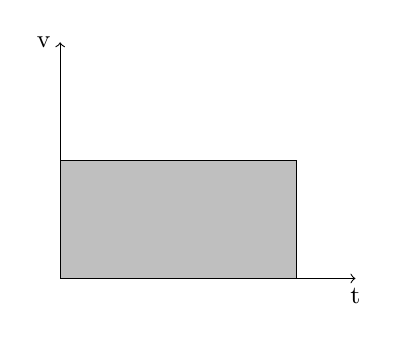
\begin{tikzpicture}[
		fatline/.style={>=latex,draw=blue,fill=blue},
		axis/.style={black,font=\small},
		linebase/.style={fill=lightgray},
		scale= 3
	]
		\draw[axis,->] (0,0) -- +(0,1) node[left] {$\uspeed$};
		\draw[axis,->] (0,0) -- +(1.25,0) node[below] {$\utime$};
		\draw[draw=black, fill=lightgray] (0, 0) rectangle(1,0.5);
	\end{tikzpicture}
	\caption{Flatarmálið undir grafinu gefur vegalengdina sem hefur verið ferðast.}
\end{figure}
%
\begin{figure}[!ht]
	\label{motion1d:fig:speedtimeareanonlinear}
	\centering
%	\includegraphics[width=0.25\textwidth]{./pictures/motion/motion_speed_time_nonlinear.eps}
	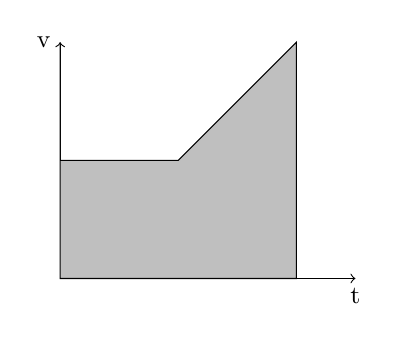
\begin{tikzpicture}[
		fatline/.style={>=latex,draw=blue,fill=blue},
		axis/.style={black,font=\small},
		linebase/.style={fill=lightgray},
		scale= 3
	]
		\draw[axis,->] (0,0) -- +(0,1) node[left] {$\uspeed$};
		\draw[axis,->] (0,0) -- +(1.25,0) node[below] {$\utime$};
		\draw[draw=black, fill=lightgray] (0, 0.5) -- ++(0.5,0) -- ++(0.5,0.5) 
			-- ++(0, -1) -- ++ (-1, 0) -- ++(0,1);
	\end{tikzpicture}
	\caption{Þrátt fyrir hraðabreytingu seinna meir á ferlinum gildir ennþá að
		flatarmálið undir graftinu gefur vegalengdina sem hefur verið ferðast,
		það getur oft orðið talsvert flókið að finna flatarmálið á hraða-tíma
		gröfum.}
\end{figure}
%
Sem sagt er hægt að meta hversu langt hlutur ferðast einunigs útfrá hraða-tíma
gröfum, hins vegar gildir \emph{ekki} það sama um stöðu-tíma gröf. Það sem við 
getum útleitt með hraða-grafi fyrir hlut sem hefur sömu hröðun (jöfn
hröðun) er vegalengdin sem er búið að ferðast, 
sjá mynd \ref{motion1d:fig:speedtimeconstaccle}. Sem er hægt að
setja sem jöfnu
\begin{equation}
	\Delta \ulengths = \uspeed_\text{byr} \utime 
		+ \frac{1}{2} \left(\uspeed_\text{loka} - \uspeed_\text{byr} \right) \utime
		= \uspeed_\text{byr} \utime + \Delta \uspeed \cdot \utime
\end{equation}
eða líka hægt að umskrifa til að vera
\begin{equation} \label{motion1d:eqn:constacceletime}
	\Delta \ulengths = \uspeed_\text{byr} \utime 
		+ \frac{1}{2} \uaccelea \utime^2
\end{equation}
sem er líka nefnd oft stöðujafna. 
\begin{figure}[!ht]
	\centering
	%\includegraphics[width=0.25\textwidth]{./pictures/motion/motion_speed_time_increasing.eps}
	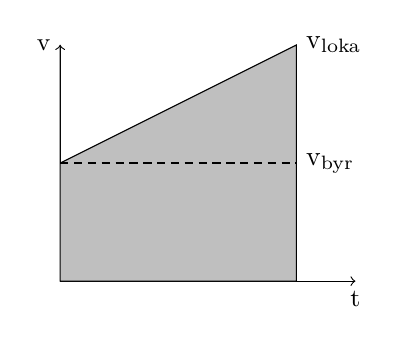
\begin{tikzpicture}[
		fatline/.style={>=latex,draw=blue,fill=blue},
		axis/.style={black,font=\small},
		linebase/.style={fill=lightgray},
		scale= 3
	]
		\draw[axis,->] (0,0) -- +(0,1) node[left] {$\uspeed$};
		\draw[axis,->] (0,0) -- +(1.25,0) node[below] {$\utime$};
		\draw[draw=black, fill=lightgray] (0, 0.5) -- ++(1.0,0.5) 
			-- ++(0, -1) -- ++ (-1, 0) -- ++(0,1);
		\draw[] (0,0) ++(1,1) node[right] {$\uspeed_\text{loka}$};
		\draw[densely dashed, draw=black] 
			(0,0.5) -- ++(1,0) node[right] {$\uspeed_\text{byr}$};
	\end{tikzpicture}
	\caption{Hérna sést hvernig hægt er að deila hraða-tíma grafi í þríhyrning
		og ferhyrning.}
	\label{motion1d:fig:speedtimeconstaccle}
\end{figure}
%
\begin{formalexample}
Bíll er á $\SI{54}{\km\per\hour}$ 
hraða, bíllinn bremsar niður í  $\SI{18}{\km\per\hour}$
hraða og það tekur $\SI{3.2}{\s}$. 
Hversu langt ferðast bíllinn á meðan hann er að bremsa?
\\[4 ex]
Byrjum á því að breyta í SI-einingar, 
$\SI{54}{\km\per\hour} = \SI{15}{\m\per\s}$
og $\SI{18}{\km\per\hour} = \SI{5}{\m\per\s}$. 
Við nýtum
\begin{align*}
	\Delta\ulengths & =  \uspeed_\text{byr} \utime 
			+ \frac{1}{2} \left(\uspeed_\text{loka} - \uspeed_\text{byr} \right) \utime
			\\
		& = \SI{15}{\m\per\s} \times \SI{3.2}{\s}
			+ \frac{1}{2} \times
				\left(
					\SI{5}{\m\per\s} - \SI{15}{\m\per\s} 
				\right) \times \SI{3.2}{\s}
			\\
		& = \SI{48}{\m} - \SI{16}{\m} \\
		& = \SI{32}{\m}
\end{align*}
\end{formalexample}
%
\begin{formalexample}
Bíll er á $\SI{54}{\km\per\hour}$ hraða, bíllinn eykur hraða sinn með hröðuninni
$\SI{3}{\m\per\s\squared}$ í $\SI{3.4}{\s}$.  
Hversu langt ferðast bíllinn á meðan hann eykur hraða sinn?
\\[4 ex]
Byrjum á því að breyta í SI-einingar, 
$\SI{54}{\km\per\hour} = \SI{15}{\m\per\s}$.
Við nýtum
\[
	\Delta\ulengths = \uspeed_\text{byr} \utime 
			+ \frac{1}{2} \uaccelea \utime
		= \SI{15}{\m\per\s} \times \SI{3.4}{\s}
			+ \frac{1}{2} \times 
				\SI{3}{\m\per\s\squared}
				\times \left( \SI{3.4}{\s} \right)^2
		= \SI{69.4}{\m}
\]
\end{formalexample}

\section{Hraðabreytingar og hröðun}
Þegar jöfn hröðun á sér stað, þá er hægt lýsa breytingunni án þess að nota
tíma sem lýsingu. Tíminn sem tekur fyrir hlut að auka hraða sinn jafnt er
\[
	\uspeed_\text{loka} = \uspeed_\text{byrjun} + \uaccelea \Delta\utime
		\Leftrightarrow
		\Delta\utime = \frac{\uspeed_\text{loka} - \uspeed_\text{byr}}{\uaccelea}
\]
ef við setjum þessa stærð inní stöðujöfnuna~\ref{motion1d:eqn:constacceletime} 
fæst
\begin{align*}
	\Delta\ulengths &= \uspeed_\text{byr} \utime 
		+ \frac{1}{2} \uaccelea \utime^2 
		&&\Leftrightarrow \\
	\Delta\ulengths &= \uspeed_\text{byr} \frac{\uspeed_\text{loka} - \uspeed_\text{byr}}{\uaccelea}
		+ \frac{1}{2} \uaccelea \left(\frac{\uspeed_\text{loka} - \uspeed_\text{byr}}{\uaccelea}\right)^2 
		&&\Leftrightarrow \\
	\Delta\ulengths &=  \frac{\uspeed_\text{loka}\uspeed_\text{byr} - \uspeed_\text{byr}^2}{\uaccelea}
		+ \frac{\left(\uspeed_\text{loka} - \uspeed_\text{byr}\right)^2}{2\uaccelea} 
		&&\Leftrightarrow \\
	2\uaccelea \Delta\ulengths &=  2\uspeed_\text{loka}\uspeed_\text{byr} - 2\uspeed_\text{byr}^2
		+ \left(\uspeed_\text{loka} - \uspeed_\text{byr}\right)^2
		&&\Leftrightarrow \\
	2\uaccelea \Delta\ulengths &=  2\uspeed_\text{loka}\uspeed_\text{byr} - 2\uspeed_\text{byr}^2
		+ \uspeed_\text{loka}^2 - 2\uspeed_\text{loka}\uspeed_\text{byr} + \uspeed_\text{byr}^2
		&&\Leftrightarrow \\
	2\uaccelea \Delta\ulengths &=  \uspeed_\text{loka}^2 - \uspeed_\text{byr}^2
\end{align*}
þeas. við höfum þá jöfnuna
\begin{equation} \label{motion:eqn:speedacceledist}
	2\uaccelea \Delta\ulengths =  \uspeed_\text{loka}^2 - \uspeed_\text{byr}^2
\end{equation}
sem getur lýst hraða, hröðun eða vegalengd hluta undir jafnri hröðun.
%
\begin{formalexample}
Bíll er á $\SI{54}{\km\per\hour}$ hraða, bíllinn eykur hraða sinn með hröðuninni
$\SI{3}{\m\per\s\squared}$ uppí hraðan $\SI{90}{\km\per\hour}$.  
Hversu langt ferðast bíllinn á meðan hann eykur hraða sinn?
\\[4 ex]
Byrjum á því að breyta í SI-einingar, 
$\SI{54}{\km\per\hour} = \SI{15}{\m\per\s}$ og
$\SI{90}{\km\per\hour} = \SI{25}{\m\per\s}$
Við umskrifum \ref{motion:eqn:speedacceledist} til að vera
\[
	2\uaccelea \Delta\ulengths =  \uspeed_\text{loka}^2 - \uspeed_\text{byr}^2
		\Leftrightarrow
		\Delta\ulengths = \frac{\uspeed_\text{loka}^2 - \uspeed_\text{byr}^2}{2\uaccelea}
			= 
				\frac{
					\left( \SI{25}{\m\per\s} \right)^2 
					- \left( \SI{15}{\m\per\s} \right)^2
					}{
					\num{2} \times \SI{3}{\m\per\s\squared}
					}
			= \SI{66.7}{\m}
\]
\end{formalexample}

\section[Línulegar jöfnur]{Hraði og línulegar jöfnur}
Hægt er að setja upp sett af línulegum jöfnum til að lýsa því hvað það tekur
langan tíma fyrir hluti að ná hvort öðru, t.d. bíll sem tekur frammúr öðrum bíl.
Til að lýsa því þá verður staðsetning hvers hlutar gefin með
\[
	\ulengths_\text{loka} = \uspeed \Delta\utime + \ulengths_\text{byrjun}
\]
gott er að muna að $\Delta \ulengths = \ulengths_\text{loka} 
- \ulengths_\text{byrjun}$.
Sem er staðsetning eins hlutarins, þá er hægt að setja upp tvær jöfnur
\begin{align*}
	\ulengths_\text{loka,A} &= \uspeed_\text{A} \Delta\utime 
		+ \ulengths_\text{byrjun,A} \\
	\ulengths_\text{loka,B} &= \uspeed_\text{B} \Delta\utime 
		+ \ulengths_\text{byrjun,B}
\end{align*}
báðar jöfnunar hafa sameiginlegan tíma sem er hægt að nýta til að leysa út eða tengja saman.
Fyrir lengra komna er hægt að sjá þessa sem fylki í hliðarrúmi%
~\footnote{S.s.  $\vec{\ulengths}_\text{loka} 
= \vec{\uspeed} \cdot \Delta\utime + \vec{\ulengths}_\text{byrjun} $}.
Það eru til nokkrar útfærslur á því hvernig hægt er að leysa þessar jöfnur.

\begin{formalexample}
Tveir bílar ferðast með jöfnum hraða, bíll A ferðast á $\SI{20}{\m\per\s}$ og 
bíll B ferðast með $\SI{15}{\m\per\s}$, bíll B er með $\SI{80}{\m}$ 
forskot miðað við A.
Hversu langan tíma tekur það fyrir bíl A að taka frammúr bíl B?
\\[4 ex]
Báðir bílarnir hafa staðsetningu miðað við núllpunkt bíls A til að vera
\begin{align*}
	\ulengths_\text{loka,A} &= 
		\SI{20}{\m\per\s} \times \Delta\utime + \SI{0}{\m} \\
	\ulengths_\text{loka,B} &= 
		\SI{15}{\m\per\s} \times \Delta\utime + \SI{80}{\m}
\end{align*}
þegar bíll A nær bíl B þá er staðsetning beggja sú sama
\begin{align*}
	\ulengths_\text{loka,A} &= \ulengths_\text{loka,B}\\
	\SI{20}{\m\per\s} \times \Delta\utime + \SI{0}{\m}
		&= \SI{15}{\m\per\s} \times \Delta\utime + \SI{80}{\m}\\
	\SI{20}{\m\per\s} \times \Delta\utime 
		- \SI{15}{\m\per\s} \times \Delta\utime 
		&=  \SI{80}{\m} \\
	\left( 
		\SI{20}{\m\per\s} - \SI{15}{\m\per\s} \right) \Delta\utime 
			&= \SI{80}{\m} \\
	\left( \SI{5}{\m\per\s} \right) \Delta\utime &=  \SI{80}{\m} \\
	\Delta\utime &=  \frac{ \SI{80}{\m} }{ \SI{5}{\m\per\s} }\\
		&=  \SI{16}{\s}
\end{align*}
\end{formalexample}

\begin{formalexample}
Bíll A bíður á ljósum og bíll B fer frammhjá með hraðanum $\SI{15}{\m\per\s}$, 
bíll A hefur hröðunina $\SI{2}{\m\per\s\squared}$ og hraðar sér upp í hraðan 
$\SI{20}{\m\per\s}$, hversu lengi er bíll A að ná bíl B?
\\[4 ex]
Til að byrja með er gott að athuga hvort að bíll A nær bíl B á meðan hröðun stendur,
það tekur bíl A að hraða sér frá kyrrstöðu upp í $\SI{20}{\m\per\s}$ nákvæmlega 
$\SI{10}{\s}$. Þá hafa bílarnir ferðast
\begin{align*}
	\ulengths_\text{hröð,A} 
		&= \frac{1}{2} \times \SI{2}{\m\per\s\squared} \times 
			\left( \SI{10}{\s} \right)^2 = \SI{100}{\m} \\
	\ulengths_\text{hröð,B} 
		&= \SI{15}{\m\per\s} \times \SI{10}{\s} 
		= \SI{150}{\m}
\end{align*}
báðir bílarnir hafa staðsetningu miðað við núllpunkt bíls A til að vera
\begin{align*}
	\ulengths_\text{loka,A} 
		&= \SI{20}{\m\per\s} \times \Delta\utime + \SI{100}{\m} \\
	\ulengths_\text{loka,B} 
		&= \SI{15}{\m\per\s} \times \Delta\utime + \SI{150}{\m}
\end{align*}
þegar bíll A nær bíl B þá er staðsetning beggja sú sama
\begin{align*}
	\ulengths_\text{loka,A} &= \ulengths_\text{loka,B}\\
	\SI{20}{\m\per\s} \times \Delta\utime + \SI{100}{\m}
		&= \SI{15}{\m\per\s} \times \Delta\utime + \SI{150}{\m} \\
	\SI{20}{\m\per\s} \times \Delta\utime 
		- \SI{15}{\m\per\s} \times \Delta\utime 
		&= \SI{50}{\m} \\
	\left( 
		\SI{20}{\m\per\s} - \SI{15}{\m\per\s} 
	\right) \Delta\utime 
		&=  \SI{50}{\m} \\
	\left( \SI{5}{\m\per\s} \right) \Delta\utime 
		&=  \SI{50}{\m} \\
	\Delta\utime 
		&=  \frac{ \SI{50}{\m} }{ \SI{5}{\m\per\s} }\\
		&=  \SI{10}{\s}
\end{align*}
þá er samanlagður tími sem er í að ná bíl B
\[
	\Delta\utime = \Delta\utime_\text{hröðun} + \Delta\utime_\text{jafn}
		= \SI{10}{\s} + \SI{10}{\s} = \SI{20}{\s}
\]
\end{formalexample}

% force
\chapter{Kraftar}
% Intro to chapter 
Fyrst skilgreinum við hvað tregða er, það er mótþrói hlutar til að breyta
hraða sínum. Hlutur á hreyfingu hefur innbyggða tregðu sem lætur hlut halda
áfram í þá stefnu og hraða sem þegar hefur. Það sem getur breytt stefnu og hraða
hlutar eru kraftar og síðan eru nokkur lögmál sem voru framsett af Newton
sem lýsa þeim eiginleikum sem láta hlutir hafa áhrif á hvorn annan.
\begin{formaltext}
	\begin{description}
		\item[1. Tregða] Hlutur sem er á hreyfingu mun halda áfram í þá stefnu sem
			hann hefur, ásamt því að halda hraða sínum óbreyttum, nema kraftur
			breyti stefnu og/eða hraða hanns. Stærð tregðu, þ.e.a.s. mótþrói við
			breytingu í hreyfingu er skriðþungi, sem er margfeldi massa og hraða.
		\item[2. Kraftur] Kraftur er margfeldi, massa og hröðunar, enginn kraftur
			verkar ef hlutur er á jöfnum hraða og heldur sömu stefnu.
		\item[3. Gagnkraftur] Fyrir hvern kraft sem verkar á hlut, er jafnstór
			og gagnstæður kraftur sem verkar samtímis.
	\end{description}
\end{formaltext}
og til að byrja með er lögð áhersla á krafta fremur en tregðu og skriðþunga.
Frá öðru lögmáli Newtons er hægt að tala um mismunandi gerðir krafta sem allir
gegna hlutverki þegar reynt er að lýsa hegðun hluta, t.d. eru nokkrir
\begin{itemize}
	\item togkraftur
	\item þyngdarkraftur
	\item heildarkraftur
	\item núningskraftur
	\item rafkraftur
	\item segulkraftur
\end{itemize}
og þetta eru ekki allar mögulegar týpur af kröftum sem finnast. Allir kraftar
hafa eininguna $\unewton$ sem er SI-eining. Það er líka hægt að að skrifa kraft
sem $\ukilo\ugramm \uaccelems$.
% Forces one dimension
\section{Heildarkraftur}
Við getum skilgreint krafta til að vera $\uforce = \umass \uaccelea$, en
þegar við leggjum saman alla mismunandi krafta þá myndast \emph{heildarkraftur}.
Þá er allt talið saman, togkraftar, núningskraftar, þyngdarkraftar, o.s.f., til
að mynda kraft sem lýsir endanlegri hreyfingu hluta í lokuðu kerfi.
Heildarkrafturinn er gefinn sem summa allra krafta fyrir \emph{einn} hlut:
\begin{equation}
	\uforce_\text{heild} = \sum \text{allir kraftar} = \umass \uaccelea
\end{equation}
til að byrja með virkar þetta sem mjög óáhugaverð jafna en mun verða
talsvert hagnýtin með tímanum og sýnir styrk lögmála Newtons\footnote{
Táknið $\sum$ þýðir samanlagning, notast til að tákna
samanlagningu á stærðum (eða kröftum hér) }. 
\begin{center}
	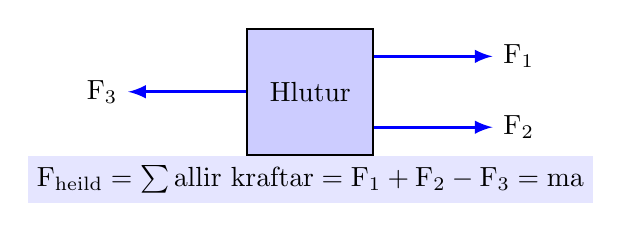
\begin{tikzpicture}[
		scale=1.5, 
		place/.style={rectangle,draw=black,fill=blue!20,thick,
		inner sep=0pt,minimum size=16mm},
		force/.style={>=latex,draw=blue,fill=blue, very thick, ->}
		]
		\node[place] (m) at (0,0) {Hlutur};
		\draw[force] (m.east) ++(0, 3mm)  -- ++(1,0) node[right] {$\uforce_1$};
		\draw[force] (m.east) ++(0, -3mm)  -- ++(1,0) node[right] {$\uforce_2$};
		\draw[force] (m.west) -- ++(-1,0) node[left] {$\uforce_3$};
		\node[below, fill=blue!10] (t) at (m.south)
			{
				$\uforce_\text{heild} 
					= \sum \text{allir kraftar} 
					=  \uforce_1 + \uforce_2 - \uforce_3
					= \umass \uaccelea
				$
			};
	\end{tikzpicture}
\end{center}
Aðalatriði í
beitingu heildarkraftsins er að velja sér hnitakerfi og byrja skilgreina
hvar mismunandi kraftar verka á ákveðin hlut. Þegar sagt er hnitakerfi
er átt við að velja hvað er jákvæð stefna í hreyfingu í láréttu og lóðréttu.
Til að reyna sýna hvernig á beita heildarkrafti er best að nýta sér
sýnidæmi.
\begin{formalexample}
Við höfum $\SI{10}{\kilo\gram}$ kassa sem liggur á borði, og er dreginn af 
$\SI{20}{\newton}$ krafti og það er $\SI{5}{\newton}$ kraftur sem verkar á móti hreyfingu 
kassans. Hver er heildarkrafturinn? Hver er hröðun kassans?
\\[4 ex]
Heildarkrafturinn er summa togkrafts $\SI{20}{\newton}$ og mótkraftur er 
$\SI{5}{\newton}$
sem gefur
\[
	\uforce_\text{heild} = \uforce_\text{tog} - \uforce_\text{mót}
		= \SI{20}{\newton} - \SI{5}{\newton} = \SI{15}{\newton}
\]
þar sem heildarkraftur er $\uforce_\text{heild} = \umass\uaccelea$, þá er hægt
að einangra hröðun hlutarins
\[
	\uforce_\text{heild} = \umass\uaccelea 
		\Leftrightarrow
		\uaccelea = \frac{\uforce_\text{heild}}{\umass}
			= \frac{ \SI{15}{\newton} }{ \SI{10}{\kilo\gram} }
			= \SI{1.5}{ \meter\per\second\squared }
\]
sem er þá hröðun kassans þegar allir kraftar eru taldir saman.
\end{formalexample}

\begin{formalexample}
Við höfum $\SI{1}{\kilo\gram}$ kúlu sem hangir í lausu lofti í bandi, og er toguð upp
með $\SI{20}{\newton}$ krafti, þyngdarkrafturinn verkar á móti
togkraftinum með stærðinni $\SI{9.8}{\newton}$. 
Hver er heildarkrafturinn? Hver er hröðun kúlunnar?
\\[4 ex]
Heildarkrafturinn er summa togkrafts $\SI{20}{\newton}$ og þyngdarkrafts sem 
er $\SI{9.8}{\newton}$
sem gefur
\[
	\uforce_\text{heild} = \uforce_\text{tog} - \uforce_\text{g}
		= \SI{20}{\newton} - \SI{9.8}{\newton} = \SI{10.2}{\newton}
\]
þar sem heildarkraftur er $\uforce_\text{heild} = \umass\uaccelea$, þá er hægt
að einangra hröðun hlutarins
\[
	\uforce_\text{heild} = \umass\uaccelea 
		\Leftrightarrow
		\uaccelea = \frac{\uforce_\text{heild}}{\umass}
			= \frac{
				\SI{10.2}{\newton}
				}{
				\SI{1}{\kilo\gram}
				}
			= \SI{10.2}{\meter\per\second\squared}
\]
sem er þá hröðun kúlunnar þegar allir kraftar eru taldir saman.
\end{formalexample}
aftur á móti eru nokkur önnur sértilfelli af þessu lögmáli. \emph{Þegar við tölum um
jafnan hraða getum við sagt að hraði hlutar helst óbreyttur}. Þetta gefur að
\[
	\uforce_\text{heild} = \umass \cdot \SI{0}{\meter\per\second\squared} 
		= \SI{0}{\newton}
\]
sem gildir bara fyrir hluti sem ferðast með \emph{óbreyttum} hraða. Sem dæmi er
\begin{formalexample}
Við höfum $\SI{1}{\kilo\gram}$ kúlu sem hangir í lausu lofti í bandi, og er toguð upp
með krafti og heldur kúlunni á jöfnum hraða, þyngdarkrafturinn verkar á móti
togkraftinum með stærðinni $\SI{9.8}{\newton}$. 
Hver er togkrafturinn? 
\\[4 ex]
Heildarkrafturinn er summa togkrafts og þyngdarkrafts sem er 
$\SI{9.8}{\newton}$, 
samanlagt verður heildarkrafturinn $\SI{0}{\newton}$ til að halda
kúlunni á jöfnum hraða. Sem gefur
\[
	\uforce_\text{heild} = \uforce_\text{tog} - \uforce_\text{g} = \SI{0}{\newton}
	\Leftrightarrow
	\uforce_\text{tog} - \SI{9.8}{\newton} = \SI{0}{\newton}
	\Leftrightarrow
	\uforce_\text{tog} = \SI{9.8}{\newton}
\]
þ.e.a.s. togkrafturinn er jafn stór og þyngdarkrafturinn ef við höldum kúlunni
á jöfnum hraða. Athugið að jafn hraði oft losar sig við fullt af vandamálum og
einfaldar talsvert kraftasamhengi.
\end{formalexample}

\section{Þyngdarkraftur}
Stærð þyngdarkraftsins er í samræmi við massa hlutars, þetta er langdregin leið
til að segja hlutur með meira massa veldur stærri þyngdarkrafti. Mátinn sem við
getum lagt fram stærð þyngdarkrafts sem er:
\begin{equation}
	\uforce_\text{\uacceleg} = \umass \uacceleg
\end{equation}
þar sem $\uacceleg = \SI{9.8}{\meter\per\second\squared}$. 
\begin{center}
	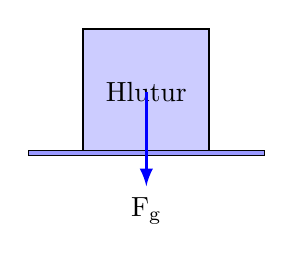
\begin{tikzpicture}[
		scale=1.5, 
		place/.style={rectangle,draw=black,fill=blue!20,thick,
		inner sep=0pt,minimum size=16mm},
		force/.style={>=latex,draw=blue,fill=blue, very thick, ->}
		]
		\node[place] (m) at (0,0) {Hlutur};
		\draw[fill = blue!40] (m.south) 
			++(-10mm, 0mm) 
			rectangle(10mm, -5mm)
			; 
		\draw[force] (m.center) -- ++(0,-8mm) node[below] {$\uforce_\uacceleg$};
	\end{tikzpicture}
\end{center}
Þá er einungis að ræða um hröðun sem hlutur
upplifir vegna þyngdarsviðs jarðar (og á yfirborði jarðar samtímis).
Þyngdarhröðun er breytileg milli pláneta, þess vegna er talað um \emph{þyngd} 
hlutars í Newtons og \emph{massa} hlutar í kílógrömmum. Massi hlutar er óháður 
þyngdarsviðinu, en þyngdin er háð styrk þyngdarsviðsins.
\begin{formalexample}
Við höfum $\SI{5}{\kg}$ kúlu sem hangir í lausu lofti í bandi, og er toguð upp
með krafti og heldur kúlunni á jöfnum hraða. Hver er togkrafturinn? 
\\[4 ex]
Við getum nýtt fyrri dæmi þar sem kúlan er á \emph{jöfnum} hraða, þá er hægt að segja
\[
	\uforce_\text{tog} = \uforce_\text{g}
\]
og þar sem við höfum nýlega skilgreint stærð þyngdarkrafts, þá er
\[
	\uforce_\text{tog} = \uforce_\text{g} = \umass \uacceleg 
		= \SI{5}{\kg} \times \SI{9.8}{\meter\per\second\squared}
		= \SI{49}{\newton}
\]
\end{formalexample}

\section{Þverkraftur}
Þegar kraftur verkar á yfirborð hluta, þá myndast gagnstæður kraftur sem er 
kallaður þverkraftur. Til samanburðar, ef bók liggur á borði, þá er það
þverkrafturinn sem sér til þess að bókin dettur ekki í gegnum borðið. Í raun
er þverkraftur form af þriðja lögmáli Newtons.
\begin{formalexample}
Við höfum kyrrstæðan kassa sem liggur á borði (á láréttu plani), kassinn 
er $\SI{10}{\kg}$.
Hver er stærð þverkraftsins?
\\[4 ex]
Þar sem kassinn er kyrrstæður, þá getum við sagt að heildarkrafturinn meðfram
hinu lóðrétta sé núll. S.s. kassinn eykur hvorki hraðan sinn upp né niður. Sem
gefur að
\[
	\uforce_\text{heild} = \uforce_\text{þver} - \uforce_\text{g} 
		= \SI{0}{\newton}
	\Leftrightarrow \uforce_\text{þver} = \uforce_\text{g}
\]
og þar sem við þekkjum massa kassans þá er hægt að setja
\[
	\uforce_\text{þver} = \uforce_\text{g} 
		= \umass \uacceleg
		= \SI{10}{\kg} \times \SI{9.8}{\meter\per\second\squared}
		= \SI{98}{\newton}
\]
sem er þá þverkrafturinn sem kassinn upplifir vegna þyngdarkraftsins.
\end{formalexample}

\section{Núningskraftur}
Þegar hlutir ferðast yfir yfirborð, þá myndast kraftur verkar á
móti hreyfingu hlutarins. Sá kraftur kallast \emph{núningskraftur} og er í
hlutfalli við stærð þverkraftsins. Til að lýsa hversu stór prósenta af
þverkraftinum nýtist til að verða núningskraftur höfum við núningsstuðullinn 
$\mu$. Sem er notaður í samhengið
\begin{equation}
	\uforce_\text{nún} = \mu \uforce_\text{þver}
\end{equation}
núningskrafturinn sjálfur er afleiða þess að draga hlut eftir yfirborði. Ef
hluturinn er ekki á hreyfingu (eða reynir ekki að hreyfa sig) þá myndast ekki
núningskraftur. Ber að athuga núningsstuðullinn er \emph{einingarlaus} stærð, 
sem liggur á milli núll og einn.
\begin{formalexample}
Kassi er togaður áfram með jöfnum hraða á borði, núningsstuðull á milli borðs
og kassa er $0,4$, massi kassans er $\SI{5}{\kg}$.
Hver er stærð togkraftsins?
\\[4 ex]
Þar sem kassinn er á jöfnum hraða er $\uforce_\text{nún} = \uforce_\text{tog}$,
og þar sem kassinn liggur í láréttu plani þá er $\uforce_\text{þver} 
= \uforce_\text{nún}$. Sem gefur að
\[
	\uforce_\text{tog} = \uforce_\text{nún} 
		= \mu \uforce_\text{þver}
		= \mu \uforce_\text{g}
		= \mu \umass \uacceleg
		= 0,4 \times \SI{5}{\kg} \times \SI{9.8}{\meter\per\second\squared}
		= \SI{19.6}{\newton}
\]
sem gildir einungis í lárréttu plani með kassa á jöfnum hraða.
\end{formalexample}

\section{Gagnkraftur}
Sem stærð kemur hún sjálfkrafa þegar kraftur verkar á hlut, gagnkraftur sér til þess
að þegar kraftur verkar á hlut muntu finna fyrir því að kraftur sé beittur. Sem dæmi
er hægt að ímynda sér að ýta kassa úr kyrrstöðu, ef þú verkar á kassann með krafti þá ferðast
hluturinn áfram en ef það væri \emph{enginn} kraftur sem verkaði á móti myndi sá sem
ýtir kassanum ekki finna fyrir því. Sem er ókunnugt frá daglegri reynslu, ef ýtt er á
kassa þá finnst kraftur á móti, sem er kunnugt frá daglegri reynslu.

\begin{formalexample}
\begin{wrapfigure}{r}{0.25\textwidth}
	\vspace{-20pt}
	\begin{center}
	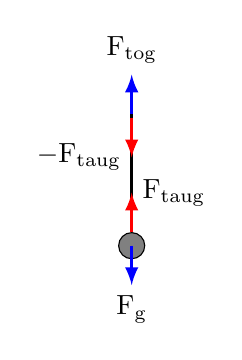
\begin{tikzpicture}[
		force/.style={>=latex,draw=blue,fill=blue, very thick},
		m/.style={circle,draw=black,fill=gray,minimum size=0.3cm,thin},
		scale=1
	]
		\node[m] (m) at (0,0) {};
		\draw[very thick, draw=black] (m.north) -- +(0,1.5);
		\draw[force, ->] (m.north) ++(0,1.5) -- +(0,0.50) node[above] {$\uforce_\text{tog}$};
		\draw[force, ->] (m.center) -- +(0,{-0.50}) node[below] {$\uforce_\uacceleg$};
		\draw[force, draw=red, fill=red, ->]
			(m.north) ++(0,1.45) -- +(0,{-0.50}) node[left] {$-\uforce_\text{taug}$};
		\draw[force, draw=red, fill=red, ->]
			(m.north) -- +(0,{0.50}) node[right] {$\uforce_\text{taug}$};
	\end{tikzpicture}
	\end{center}
	\vspace{-10pt}
\end{wrapfigure}
Kúla hangir í bandi, enda bandsins er haldið fast. Kúlan hefur massann 
$\SI{5}{\kg}$.
Sýndu stefnu og stærð allra krafta og gagnkrafta.
\\[4 ex]
Þar sem endinn á bandinu er haldið fast, þá er heildarkrafturinn núll, ef við skoðum
bara endann á bandinu þá eru kraftarnir verka á enda bandsins
\[
	\uforce_\text{heild,endi} = \uforce_\text{tog} - \uforce_\text{taug} 
	= \SI{0}{\newton} 
\]
og þar sem kúlan hengur í hinum endanum er
\[
	\uforce_\text{heild,kúla} = \uforce_\text{taug} - \uforce_\text{g} 
	= \SI{0}{\newton}
\]
núna er hægt að búa til heildar-kraftsmynd þar sem allir kraftarnir eru lagðir saman.
Ef við leggjum alla kraftana saman á samtímis
\begin{align*}
	\uforce_\text{heild} &= \uforce_\text{tog} 
		+ \uforce_\text{taug} 
		- \uforce_\text{taug} - \uforce_\text{g}
	= 0 \\
	\uforce_\text{heild} &= \uforce_\text{tog} 
		- \uforce_\text{g}
	= 0 \\
	\uforce_\text{tog} &= \uforce_\text{g}
\end{align*}
sem gefur að togkrafturinn er
\[
	\uforce_\text{tog} = \uforce_\text{g} = \umass \uacceleg 
		= \SI{5}{\kg} \times \SI{9.8}{\meter\per\second\squared}
		= \SI{49}{\newton}
\]
\end{formalexample}

\subsection{Heildarkraftur á stór kerfi}
Hingað til hefur verið unnið með ekki meira en einn hlut í einu, þá eru allir
kraftar sem verka á einn hlut teknir og lagðir saman til að mynda þann kraft sem
kemur ef allt er talið saman. En það er sjaldan sem það er svo einfalt
í raunveruleikanum, þá munu fleiri en einn hlutur oft taka þátt í því að mynda
heildarkraft. Nánar tiltekið þá er mikilvægt að bæta við massanum á hverjum hlut
sem er í kerfinu. Sem gefur
\begin{equation}
	\uforce_\text{heild} = \sum \text{allir kraftar} = \sum \umass \uaccelea
\end{equation}
sem þýðir að allir massar þurfa eru lagðir saman til að lýsa hreyfingu og
kröftum kerfisins, og samtímis táknar summu alla krafta. Nokkur dæmi eru heppileg til að
sýna hvernig slíkir eiginleikar lýsa sér.
\begin{formalexample}
\begin{wrapfigure}{r}{0.25\textwidth}
	\vspace{-20pt}
	\begin{center}
	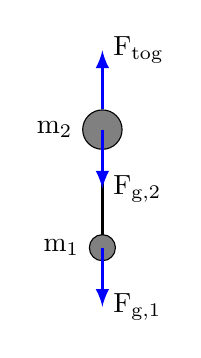
\begin{tikzpicture}[
		force/.style={>=latex,draw=blue,fill=blue, very thick},
		m1/.style={circle,draw=black,fill=gray,minimum size=0.3cm,thin},
		m2/.style={circle,draw=black,fill=gray,minimum size=0.5cm,thin},
		scale=1
	]
		\draw[very thick, draw=black] (0,0) -- +(0,1.5);
		\node[m1] (m1) at (0,0) {};
		\node[m2] (m2) at (0,1.5) {};
		\draw[] (m2.west) node[left] {$\umass_2$};
		\draw[] (m1.west) node[left] {$\umass_1$};
		\draw[force, ->] (m2.north) -- +(0,0.75) node[right] {$\uforce_\text{tog}$};
		\draw[force, ->] (m2.center) -- +(0,{-0.75}) node[right] {$\uforce_{\uacceleg,2}$};
		\draw[force, ->] (m1.center) -- +(0,{-0.75}) node[right] {$\uforce_{\uacceleg,1}$};
	\end{tikzpicture}
	\end{center}
	\vspace{-10pt}
\end{wrapfigure}
Kúlur hanga í bandi, enda bandsins er haldið fast. Kúla 1 hefur massann 
$\SI{2}{\kg}$. Kúla 2 hefur massan $\SI{5}{\kg}$. Sýndu stefnu og stærð 
allra krafta og gagnkrafta.
\\[4 ex]
Þar sem endinn á bandinu er haldið fast, þá er heildarkrafturinn núll, kraftarnir
sem verka á sitt hvora kúluna eru
\[
	\uforce_\text{heild,1} = \uforce_\text{taug} - \uforce_{\uacceleg,1} 
	= \SI{0}{\newton}
\]
og þar sem kúlan hengur í hinum endanum er
\[
	\uforce_\text{heild,2} = \uforce_\text{tog} 
		- \uforce_{\uacceleg,2} - \uforce_\text{taug} 
	= \SI{0}{\newton}
\]
núna er hægt að búa til heildar-kraftsmynd þar sem allir kraftarnir eru lagðir saman.
Ef við leggjum alla kraftana saman á samtímis
\begin{align*}
	\uforce_\text{heild} &= \uforce_\text{taug} - \uforce_{\uacceleg,1}
		+ \uforce_\text{tog} - \uforce_{\uacceleg,2} - \uforce_\text{taug}
		= \SI{0}{\newton} \\
	\uforce_\text{heild} &= \uforce_\text{tog} - \uforce_{\uacceleg,1}
		- \uforce_{\uacceleg,2} 
		= \SI{0}{\newton} \\
	\uforce_\text{heild} &= \uforce_\text{tog} - \umass_1 \uacceleg
		- \umass_2 \uacceleg
		= \SI{0}{\newton} \\
	\uforce_\text{heild} &= \uforce_\text{tog} - \SI{19.6}{\newton}
		- \SI{49}{\newton}
		= \SI{0}{\newton} \\
	\uforce_\text{tog} &= \SI{19.6}{\newton}
		+ \SI{49}{\newton}
		\\
	 &= \SI{68.6}{\newton}
\end{align*}
\end{formalexample}
Hins vegar er hægt að taka sömu aðstæður og í fyrra sýnidæmi og skoða hver
hröðunin verður ef togað er upp með krafti.
\begin{formalexample}
\begin{wrapfigure}{r}{0.25\textwidth}
	\vspace{-20pt}
	\begin{center}
	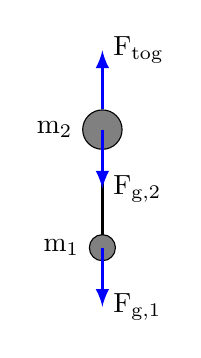
\begin{tikzpicture}[
		force/.style={>=latex,draw=blue,fill=blue, very thick},
		m1/.style={circle,draw=black,fill=gray,minimum size=0.3cm,thin},
		m2/.style={circle,draw=black,fill=gray,minimum size=0.5cm,thin},
		scale=1
	]
		\draw[very thick, draw=black] (0,0) -- +(0,1.5);
		\node[m1] (m1) at (0,0) {};
		\node[m2] (m2) at (0,1.5) {};
		\draw[] (m2.west) node[left] {$\umass_2$};
		\draw[] (m1.west) node[left] {$\umass_1$};
		\draw[force, ->] (m2.north) -- +(0,0.75) node[right] {$\uforce_\text{tog}$};
		\draw[force, ->] (m2.center) -- +(0,{-0.75}) node[right] {$\uforce_{\uacceleg,2}$};
		\draw[force, ->] (m1.center) -- +(0,{-0.75}) node[right] {$\uforce_{\uacceleg,1}$};
	\end{tikzpicture}
	\end{center}
	\vspace{-10pt}
\end{wrapfigure}
Kúlur hanga í bandi, enda bandsins er haldið fast. Kúla 1 hefur massann $\SI{2}{\kg}$.
Kúla 2 hefur massann $\SI{5}{\kg}$. Togað er í efri kúluna með 
$\SI{75}{\newton}$ krafti.
Sýndu stefnu og stærð allra krafta og gagnkrafta.
\\[4 ex]
Þar sem endinn á bandinu er haldið fast, þá er heildarkrafturinn núll, kraftarnir
sem verka á sitt hvora kúluna eru
\[
	\uforce_\text{heild,1} = \uforce_\text{taug} - \uforce_{\uacceleg,1} = \umass_\text{1} \uaccelea
\]
og þar sem kúlan hangir í hinum endanum er
\[
	\uforce_\text{heild,2} = \uforce_\text{tog} 
		- \uforce_{\uacceleg,2} - \uforce_\text{taug} = \umass_\text{2} \uaccelea
\]
núna er hægt að búa til heildar-kraftsmynd þar sem allir kraftarnir eru lagðir saman.
Ef við leggjum alla kraftana saman 
\begin{align*}
	\uforce_\text{heild} &= \uforce_\text{taug} - \uforce_{\uacceleg,1}
		+ \uforce_\text{tog} - \uforce_{\uacceleg,2} - \uforce_\text{taug}
		= \SI{0}{\newton} \\
	\uforce_\text{heild} &= \uforce_\text{tog} - \uforce_{\uacceleg,1}
		- \uforce_{\uacceleg,2} 
		= \left( \umass_\text{1} + \umass_\text{2}\right)  \uaccelea \\
	\uforce_\text{heild} &= \uforce_\text{tog} - \umass_1 \uacceleg
		- \umass_2 \uacceleg
		= \left( \umass_\text{1} + \umass_\text{2}\right)  \uaccelea \\
	\uforce_\text{heild} &= \SI{75}{\newton} - \SI{19.6}{\newton}
		- \SI{49}{\newton}
		= \left( \SI{7}{\kg} \right) \times \uaccelea \\
	\uforce_\text{heild} &= \SI{6.4}{\newton} 
		= \left( \SI{7}{\kg} \right) \times \uaccelea \\
	\uaccelea &= \frac{ \SI{6.4}{\newton} }{ \SI{7}{\kg} }
		\\
		&= \SI{0.914}{\meter\per\second\squared}
\end{align*}
\end{formalexample}

% Forces inclining plane
\section{Kraftar í skáplani}
Þegar hlutur liggur í skáplani breytast aðstæðurnar fyrir því hvernig
þyngdarkrafturinn verkar á sjálft. Í láréttu plani er hægt að miða út frá því
að allur þyngdarkrafturinn verður þverkraftur, aftur á móti í skáplani er
þverkrafturinn háður því hver hallinn er á planinu. Samhliða því myndast kraftur
sem verkar samsíða planinu. Kraftarnir hafa stærðina:
\begin{align}
	\uforce_\text{s} 
		&= \uforce_\text{g} \sin \theta \\
	\uforce_\text{þver, ská} 
		&= \uforce_\text{g} \cos \theta
\end{align}
Þá er hægt að byggja upp kraftmynd, þar sem við skoðum allt frá sjónarhorni
plansins.
\begin{figure}[h]
	\centering
	\def\iangle{25} % Angle of the inclined plane
	\def\down{-90}
	\def\arcr{0.45cm} % Radius of the arc used to indicate angles
	\begin{tikzpicture}[
		force/.style={>=latex,draw=blue,fill=blue, very thick},
		forcecomp/.style={>=latex,draw=blue, densely dashed, fill=blue},
		axis/.style={densely dashed,gray,font=\small},
		m/.style={rectangle,draw=black,fill=gray,minimum size=0.3cm,thin},
		M/.style={rectangle,draw,fill=lightgray,minimum size=0.3cm,thin},
		scale=3
	]
	\draw[fill=lightgray, draw=black]
		(0, 0) -- +(2.75,{2.75*tan(\iangle)}) -- +(2.75,0) -- cycle;
	
	\begin{scope}[rotate=\iangle, yshift=0.15cm, xshift={2.5cm/cos(\iangle)*0.75}, scale=1.0]
		\node[M,transform shape] (M) {};
		% Draw axes and help lines
		% Forces
		{[force,->]
			% Assuming that Mg = 1. The normal force will therefore be cos(alpha)
			\draw[force, ->] (M.south) ++(0.1,0) -- +(0,{cos(\iangle)}) node[above] {$\uforce_\text{þver, ská}$};
			\draw[force, ->] (M.center) -- ++({-sin(\iangle)},0) node[left] {$\uforce_\text{s}$};
			\draw[force, ->] (M.center) -- ++(0,{-cos(\iangle)}) node[right] {$\uforce_\text{g,ská}$};
			\draw[force, ->] (M.center) -- ++({-sin(\iangle)},{-cos(\iangle)}) node[below] {$\uforce_\text{g}$};
			\draw[forcecomp] (M.center) ++({-sin(\iangle)},0) -- +(0,{-cos(\iangle)});
			\draw[forcecomp] (M.center) ++ (0,{-cos(\iangle)}) -- +({-sin(\iangle)},0);
		}
	\end{scope}
	
	\draw[solid,shorten >=0.5pt] (0,0) +(0:\arcr)
		arc(0:\iangle:\arcr);
	\node at (0+\iangle*0.5:1.25*\arcr) {$\theta$};
	\end{tikzpicture}
	\caption{Kraftar í skáplani, þar sem kassinn er áætlaður til að vera
		dreginn samsíða planinu þá er heildarkrafturinn þvert á planið núll.
		Sem þýðir $\uforce_\text{heild, þver} = \uforce_\text{þver, ská} 
		- \uforce_\text{g,ská} = 0$ og gefur $ \uforce_\text{þver, ská} 
		= \uforce_\text{g,ská}$.
		}
	\label{forces:inclinedplane:setup}
\end{figure}

\begin{formalexample}
Kassi er togaður upp plan með jöfnum hraða í skáplani, núningsstuðull á milli
skáplans og kassa er $\num{0.4}$, massi kassans er $\SI{5}{\kg}$ og halli skáplans
er $\SI{15}{\degree}$. Hver er stærð togkraftsins?
\\[4 ex]
Þar sem kassinn er á jöfnum hraða þá er
\[
	\uforce_\text{heild} = \uforce_\text{tog} - \uforce_\text{s} -\uforce_\text{nún} = 0
\]
sem gefur að togkrafturinn er $\uforce_\text{tog} = \uforce_\text{s} + \uforce_\text{nún}$. Þar
sem $\uforce_\text{nún} = \mu \uforce_\text{þver}$ og $\uforce_\text{g} = \umass \uacceleg$,
þá er hægt að setja inn
\begin{align*}
	\uforce_\text{tog} &= \uforce_\text{s} + \uforce_\text{nún} \\
		&= \uforce_\text{g} \sin \theta + \mu \uforce_\text{g} \cos \theta \\
		&= \umass \uacceleg \sin \theta + \mu \umass \uacceleg \cos \theta \\
		&= \SI{5}{\kg} \times \SI{9.8}{\m\per\s\squared} 
			\times \sin \left( \SI{15}{\degree} \right)
			+ \num{0,4} \times \SI{5}{\kg} \times \SI{9.8}{\m\per\s\squared} 
			\times \cos \left( \SI{15}{\degree} \right) 
			\\
		&= \SI{3.2}{\N}
\end{align*}
það sem er gott að muna er að þessir kraftar reiknast einungis frá sjónarhorni
plansins. Þannig séð er þetta nákvæmlega sama tilfelli eins þegar við skoðum
kassa sem dreginn í láréttu nema það kemur aukakraftur og þverkrafturinn er
flóknari í uppsetningu.
\end{formalexample}

\begin{formalexample}
Kassi rennur niður skáplan, núningsstuðull á milli
skáplans og kassa er $\num{0.25}$, massi kassans er $\SI{5}{\kg}$ og halli skáplansins
er $\SI{15}{\degree}$. Hver er hröðun kassans?
\\[4 ex]
Núna er enginn togkraftur en núningskrafturinn verkar upp planið sem gefur
\[
	\uforce_\text{heild} = \uforce_\text{nún} - \uforce_\text{s} = \umass \uaccelea
\]
til að ná betri yfirsjón, þá er hægt er hægt að reikna þessa tvo krafta nú þegar
\begin{align*}
	\uforce_\text{nún} &= \mu \umass \uacceleg \cos \theta 
		= \num{0.25} \times \SI{5}{\kg} \times \SI{9.8}{\m\per\s\squared} 
			\times \cos \left( \SI{15}{\degree} \right) 
		= \SI{11.8}{\N} \\
	\uforce_\text{s} &= \umass \uacceleg \sin \theta
		= \SI{5}{\kg} \times \SI{9.8}{\m\per\s\squared} 
			\times \sin \left( \SI{15}{\degree} \right) 
		= \SI{12.7}{\N}
\end{align*}
og við getum fundið hröðunina með
\[
	\uaccelea = \frac{\uforce_\text{nún} - \uforce_\text{s}}{\umass}
		= \frac{ \SI{11.8}{\N} - \SI{12.7}{\N}  }{ \SI{5}{\kg} }
		= - \SI{0.18}{\m\per\s\squared}
\]
neikvætt formerki táknar hér að kassinn rennur \emph{niður} skáplanið, þar sem
jákvæð hreyfistefna er skilgreind sem \emph{upp} planið.
\end{formalexample}

% momentum
\section{Skriðþungi}
Skriðþungi er stærð táknar tregðu hlutars til að breyta hraða og stefnu, sem
almenn regla er skriðþungi táknaður sem vigur stærð. Hins vegar verður einungis
kynntur skriðþungi í einni vídd, sem þýðir að formerki mun tákna stefnu og
stærð skriðþungans verður tölugildið. Í fleiri víddum þarf að nota vigra sem
verður nánar skoðað í áframhaldandi köflum. Fyrst er það skilgreiningin á
skriðþunga
\begin{equation}
	\umomentum = \umass \uspeed
\end{equation}
mikilvægi þessa jöfnu verður útlistað í framtíðarköflum, en til að byrja með
verður skoða þau tilfelli þegar hlutir breyta skriðþunga sínum. Sem er oftast
við árekstra á milli atóma, hluta, kúlna og kassa.

Það eru tvenns konar kerfi sem verða skoðuð, þegar við segjum kerfi er átt við
samansafn af hlutum sem geta verkað á hvort annað. Þegar um lokað kerfi er átt
við að skriðþunginn er varðveittur og hverfur ekki, opið kerfi myndi leyfa massa
að hverfa (þ.e.a.s. hlut) og myndi ekki varðveita skriðþungan%
\footnote{Opin og lokuð kerfi gilda líka um krafta og orku, en hér er einungis
verið að skoða skriðþunga}. Það er líka hægt að tala um samanlagðan skriðþunga
kerfis, þá er skriðþungi hvers hlutar samanlagður og tekið tillit til stefnu
hlutarins.
\[
	\umomentum_\text{heild} = \sum \umomentum = \text{summa allra }\umomentum
\]
þá er táknið $\sum$ notað fyrir samanlagningu á öllum skriðþungum. Það sem gildir
í \emph{lokuðum kerfum} er það skriðþunginn breytist ekki. Sem gefur að
\[
	\umomentum_\text{heild, fyrir} = \umomentum_\text{heild, eftir}
\]
þá er samanlagður skriðþunga fyrir og eftir atvik sá sami.
%
\begin{formalexample}
Tveir bílar lenda í árekstri, bíll A er $\SI{800}{\kg}$ og á 
$\SI{54}{\km\per\hour}$ hraða,
bíll B er $\SI{1500}{\kg}$ og er á $\SI{36}{\km\per\hour}$ hraða. Þegar bílarnir
lenda saman getum áætlað að þeir festast saman og verði einn nýr heildarmassi.
Hver verður hraði nýja massanns eftir árekstur?
\\[4 ex]
Við breytum helstu stærðum í SI-einingar, $\SI{54}{\km\per\hour} 
= \SI{15}{\m\per\s}$ og $\SI{36}{\km\per\hour} = \SI{10}{\m\per\s}$. Síðan 
er stefna bílanna mikilvæg, þar sem bílarnir koma úr \emph{gagnstæðum} 
áttum þýðir að annar hefur neikvæða hreyfistefnu. Ef við áætlum að bíll 
A ferðast í jákvæða stefnu, þá ferðast bíll B í neikvæða stefnu. Þar 
sem við getum fundið heildarskriðþunga fyrir og eftir árekstur, þá er 
heildarskriðþungi fyrir árekstur
\begin{align*}
	\umomentum_\text{heild, fyrir} &= \SI{800}{\kg} \times \SI{15}{\m\per\s}
		+ \SI{1500}{\kg} \times \left( - \SI{10}{\m\per\s} \right) \\
	&= \SI{800}{\kg} \times \SI{15}{\m\per\s}
		- \SI{1500}{\kg} \times \SI{10}{\m\per\s} \\
	&= - \SI{3000}{\N\s}
\end{align*}
þegar bílarnir lenda saman er þá er samanlagður skriðþungi eftir árekstur
\begin{align*}
	\umomentum_\text{heild, eftir} &= 
		\left(\SI{800}{\kg} + \SI{1500}{\kg} \right) \times \uspeed
		\\
	&= 
		\SI{2300}{\kg} \times \uspeed
\end{align*}
þar sem skriðþunginn varðveitist er hægt að segja
\begin{align*}
	\umomentum_\text{heild, fyrir} &= 
		\umomentum_\text{heild, eftir}
		\\
	-\SI{3000}{\N\s} &= 
		\SI{2300}{\kg} \times \uspeed
		\\
	\uspeed &= 
		\frac{-\SI{3000}{\N\s} }{ \SI{2300}{\kg} }
		\\
	&=
		-\SI{1.3}{\m\per\s}
\end{align*}
hér táknar $-\SI{1.3}{\m\per\s}$ að nýi massinn (bíll A og B klesstir saman) stefna
í sömu átt og bíll B, þ.e.a.s. í gagnstæða átt við bíl A.
\end{formalexample}
%
Kraftar og skriðþungi eru nátengdar stærðir, nánar tiltekið, kraftur er afleiða
skriðþunga. Afleiða í stærðfræðilegum skilningi og reyndar almennum líka. Sem
stærð er hægt að tengja skriðþunga og kraft með
\begin{equation}
	\uforce = \frac{\Delta\umomentum}{\Delta\utime}
\end{equation}
s.s. kraftur er jafn stór og breytingin í skriðþunga á tímaeiningu. Sem passar ef
lögmál Newtons eru skoðuð nánar, til að breyta stefnu eða hraða hlutars þarf
að beita krafti. Þá hlýtur að gilda að ef hlutur breytir skriðþunga 
sínum (í stefnu eða stærð) að kraftur hafi verkað á hlutinn, 
annars hefði allt haldist óbreytt.

\subsection{Atlag}
Þegar skriðþungi breytist er hægt að lýsa því sem stærð af krafti og tíma, sem
stærð er atlag
\begin{equation}
	\Delta\umomentum = \uforce \Delta\utime 
\end{equation}
þá er það skriðþungabreyting sem er jafngildi meðalkraftsins margafaldað með
tímanum. Það er líka mikilvægt að gera grein fyrir stefnu skriðþunga, sama og
með krafta, stundum vinna kraftar með eða móti hreyfingu, skriðþungi getur unnið
með og móti hreyfingu hluta.

Sem hluti af þessu, þá er hægt að gera kraft-tíma gröf þar sem flatarmálið undir
grafinu er jafngildi skriðþungans sem hefur verið færður á milli hlutanna. Það
er sjáanlegt á stærðinni $\Delta\umomentum = \uforce \Delta\utime$ að hún svipar
til $\Delta\ulengths = \uspeed \Delta\utime$.
\begin{formalexample}
\begin{wrapfigure}{r}{0.5\textwidth}
	\begin{center}
		\centering
		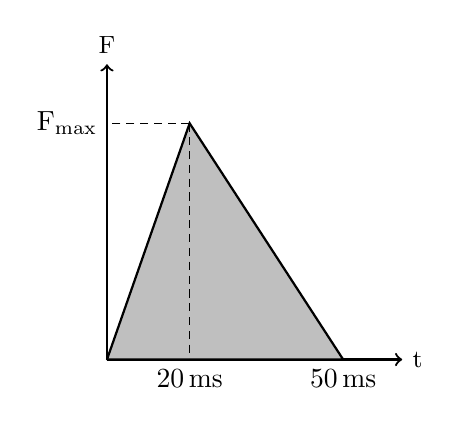
\begin{tikzpicture}[
			bline/.style={thick, fill=lightgray, draw=black},
			axis/.style={thick, draw=black, font=\small},
			scale= 3
		]
			\draw[axis,->] (0,0) -- +(1.25,0) node[right] {$\utime$};
			\draw[axis,->] (0,0) -- +(0,1.25) node[above] {$\uforce$};
			\draw[bline] (0,0) -- ++(0.35, 1) -- ++(0.65, -1) -- ++ (-1, 0);
			%\draw[densely dashed] (0,35,1) -- ++(0,-1) node[right] {$\utime$};
			\draw[draw=black, densely dashed] (0.35, 1) -- +(0,-1) 
				node[below] {$\SI{20}{\ms}$};
			\draw[draw=black, densely dashed] (0.35, 1) -- +(-0.35,0) 
				node[left] {$\uforce_\text{max}$};
			\draw[] (1, 0) 
				node[below] {$\SI{50}{\ms}$};
		\end{tikzpicture}
	\end{center}
\end{wrapfigure}
Bolti lendir á kylfu, áður en boltinn boltinn lendir á kylfunni er hraði boltans
$\SI{10}{\m\per\s}$ og eftir að boltinn lendir kylfunni er hraði boltans er
$8 \uspeedms$ og í gagnstæða átt. 
Það líða $\SI{20}{\ms}$ áður en krafturinn sem boltinn verkar
kylfuna verður stærstur og síðan líða $\SI{30}{\ms}$ þar til kylfan er búin að
verka á boltann. Massi boltans er $\SI{0.10}{\kg}$.
Hvert er hámark kraftsins sem verkar á boltann?
\\[4 ex]
Þar sem við þekkjum hraðan fyrir og eftir kylfuslagið er hægt að finna breytingu í
skriðþunga á þessum $50 \umilli\usec$. Sem gefur
\begin{align*}
	\Delta\umomentum &= \umomentum_\text{eftir} - \umomentum_\text{fyrir} \\
		&= \SI{0.1}{\kg} \times \SI{10}{\m\per\s} 
			- \left( - \SI{0.1}{\kg} \times \SI{8}{\m\per\s} \right) \\
		&= \SI{0.9}{\N\s}
\end{align*}
og allt flatarmálið undir grafinu er jafn stórt og þessi stærð, flatarmálið er gefið
sem
\begin{align*}
	\Delta\umomentum &= \frac{1}{2} \uforce_\text{max} \Delta\utime_1
		+ \frac{1}{2} \uforce_\text{max} \Delta\utime_2 \\
	\SI{0.9}{\N\s} &= 
		\frac{1}{2} \times \uforce_\text{max} \times \SI{0.020}{\s}
		+ \frac{1}{2} \times \uforce_\text{max} \times \SI{0.030}{\s} \\
	\SI{0.9}{\N\s} &=
		\left(
			\frac{1}{2} \times  \SI{0.020}{\s}
			+ \frac{1}{2} \times \SI{0.030}{\s} 
		\right) 
		\times 
		\uforce_\text{max} \\
	\SI{0.9}{\N\s} &=
		\SI{0.025}{\s} \times \uforce_\text{max} \\
	\uforce_\text{max} &=
		\frac{ \SI{0.9}{\N\s} }{ \SI{0.025}{\s} }
		= \SI{36}{\N}
\end{align*}
sem er hámarkið á kraftinum sem hefur verkað á boltann er því í beinu samræmi við hversu
lengi og hversu stór skriðþungabreytingin er.
\end{formalexample}

% momentum
\section{Kraftar sem vigrar}
Kraftar í einni vídd eru hagnýtir, nema það er oft þörf að taka mark á fleiri
en einni vídd, vídd hér er átt við hreyfistefna. Kraftur sem verkar á horni er
hægt að lýsa sem tveim kröftum sem eru hornréttir á hvorn annan. Almennt getum 
við sagt að kraftur er gefinn í hornréttu hnitakerfi er
\begin{align}
	\uforce_\text{x} &= \uforce \cos(\theta)\\
	\uforce_\text{y} &= \uforce \sin(\theta)
\end{align}
Þar sem $\uforce$ táknar stærð vigursins, $\uforce_\text{x}$ táknar stærð vigurs 
meðfram x-ás og $\uforce_\text{y}$ táknar stærð vigurs meðfram y-ás. Almennt er
hægt að gera þetta við alla vigra, ekki einungis kraftvigra, þeir vigrar sem munu
verða skoðaðir í þessum hluta eru kraftvigrar. Mynd \ref{basic:fig:twodimforces}
sýnir dæmi um hvernig kraftur er þáttum meðal ásum kerfisins.

Ef kassi er togaður áfram og togáttin er samsíða planinu sem kassi er dreginn eftir
þá fer allur togkraftur í að toga kassann áfram. Hins vegar ef kassi er dreginn
á horni við planið, þá er hluti af togkraftinum sem fer í að toga kassann áfram
og hluti fer í að lyfta kassann upp.

\begin{figure}[!htb]
\label{basic:fig:twodimforces}
\centering
\def\iangle{35} % Angle of the inclined plane
\def\down{-90}
\def\arcr{0.45cm} % Radius of the arc used to indicate angles
\begin{tikzpicture}[
	force/.style={>=latex,draw=blue,fill=blue},
	forcecomp/.style={>=latex,draw=blue, densely dashed, fill=blue},
	axis/.style={densely dashed,gray,font=\small},
	m/.style={rectangle,draw=black,fill=gray,minimum size=0.3cm,thin},
	scale= 3
]
	\node[m, transform shape] (m) {};
	\draw[force,->] (m.east) -- +({cos(\iangle)},{sin(\iangle)}) node[right] {$\uforce_\text{}$};
	% Indicate angle. The code is a bit awkward.
	\draw[forcecomp,->] (m.east) -- +({cos(\iangle)},0) node[below] {$\uforce_\text{x}$};
	\draw[forcecomp,->] (m.east) -- +(0,{sin(\iangle)}) node[left] {$\uforce_\text{y}$};
	\draw[solid,shorten >=0.5pt] (m.east) +(0:\arcr)
		arc(0:\iangle:\arcr);
	\node at (0+\iangle*0.5:1.5*\arcr) {$\theta$};
	\node[] (table) {};
	\draw[draw=black, fill=lightgray] (m.south) +(-0.5, 0) rectangle(1,-0.5);
\end{tikzpicture}
\caption{
	Kassinn er togaður áfram á horni, $\uforce_\text{x}$ og $\uforce_\text{y}$.
	Stikluðu bláu línurnar tákna kraftana sem eru meðfram hnitakerfinu.
	}
\end{figure}

Og þetta leiðir til að hægt er að deila kraftinum meðfram ásum hnitakerfisins og finna
líka heildarkraftinn sem verkar á hlutinn í tveim þáttum. S.s. við getum talað um heildarkraftinn
$\uforce_\text{heild,x}$ og $\uforce_\text{heild,y}$. 

\begin{formalexample}
\begin{wrapfigure}{r}{0.5\textwidth}
	\begin{center}
		\centering
		\def\iangle{35} % Angle of the inclined plane
		\def\down{-90}
		\def\arcr{0.45cm} % Radius of the arc used to indicate angles
			% \includegraphics[width=0.25\textwidth]{./pictures/forces/force_one_dimension_totalforce_vertical.eps}
		\begin{tikzpicture}[
			force/.style={>=latex,draw=blue,fill=blue, thick},
			forcecomp/.style={>=latex,draw=blue, densely dashed, fill=blue},
			axis/.style={densely dashed,gray,font=\small},
			m/.style={rectangle,draw=black,fill=gray,minimum size=0.3cm,thin},
			scale= 2
		]
			\node[m, transform shape] (m) {};
			\draw[force,->] (m.east) -- +({cos(\iangle)},{sin(\iangle)}) node[right] {$\uforce_\text{tog}$};
			% Indicate angle. The code is a bit awkward.
			\draw[forcecomp,->] (m.east) -- +({cos(\iangle)},0) node[right] {$\uforce_\text{tog,x}$};
			\draw[forcecomp,->] (m.east) -- +(0,{sin(\iangle)}) node[above] {$\uforce_\text{tog,y}$};
			\draw[solid,shorten >=0.5pt] (m.east) +(0:0.5*\arcr)
				arc(0:\iangle:0.5*\arcr);
			\node at (0+\iangle*0.5:1*\arcr) [right] {$20 \udeg$};
			\draw[draw=black, fill=lightgray] (m.south) +(-0.5, 0) rectangle(1,-0.5);
			\draw[force,->] (m.center) -- +(0,{-1}) node[below] {$\uforce_\text{g}$};
			\draw[force,->] (m.south west) -- +(-0.5,0) node[above] {$\uforce_\text{nún}$};
			\draw[force,->] (m.south west) ++(0.05,0) -- +(0,1) node[above] {$\uforce_\text{þver}$};
		\end{tikzpicture}
	\end{center}
\end{wrapfigure}
Kassi er togaður áfram með $\SI{50}{\N}$ krafti og á $\SI{20}{\degree}$
horni miðað við lárétt, massi kassans er $\SI{10}{\kg}$ og núningsstuðull 
á milli kassans og flatar er $\num{0.25}$. 
Hver er hröðun kassans?
\\[4 ex]
Fyrst er að finna hver heildarkrafturinn meðfram lóðrétta ásnum, við höfum þyngdarkraftinn
sem verkar niður, þverkraftinn sem verkar upp og núna kemur viðbótar $y$ þáttur frá 
togkraftinum. Heildarkrafturinn er samanlagt núll, þar sem kassinn helst á yfirborði
flatarins
\begin{align*}
	\uforce_\text{heild,y} & = \uforce_\text{tog,y} + \uforce_\text{þver} 
		- \uforce_\text{g} = 0 && \Leftrightarrow \\
	\uforce_\text{þver} & = \uforce_\text{g} - \uforce_\text{tog,y}
		&& \Leftrightarrow \\
		& = \umass \uacceleg - \uforce_\text{tog} \sin \left( \theta \right)
		&&  \\
		& = \SI{10}{\kg} \times \SI{9.8}{\m\per\s\squared} 
			- \SI{50}{\N} \times \sin \left( \SI{20}{\degree} \right)
		&&  \\
		& = \SI{98}{\N} - \SI{17}{\N} = \SI{81}{\N}
		&&  
\end{align*}
núningskrafturinn sem verkar á móti hreyfingu kassans í láréttu er
\[
	\uforce_\text{nún} = \mu \uforce_\text{þver} 
		= \num{0.25} \times \SI{81}{\N} = \SI{20}{\N}
\]
þá er heildarkrafturinn í láréttu er þá
\begin{align*}
	\uforce_\text{heild,x} & = \uforce_\text{tog,x} - \uforce_\text{nún} 
		 = \umass \uaccelea && \Leftrightarrow \\
	\uforce_\text{heild,x} & = \SI{50}{\N} 
			\times \cos \left( \SI{20}{\degree} \right)
			- \SI{20}{\N}
			= \SI{10}{\kg} \times \uaccelea 
		&& \Leftrightarrow \\
	\uforce_\text{heild,x} & = \SI{47}{\N}
			- \SI{20}{\N}
			= \SI{10}{\kg} \times  \uaccelea 
		&& \Leftrightarrow \\
	\uforce_\text{heild,x} & = \SI{27}{\N}
			= \SI{10}{\kg} \times \uaccelea 
		&& \Leftrightarrow \\
	\uaccelea & = \frac{ \SI{27}{\N} }{ \SI{10}{\kg} }
			= \SI{2.7}{\m\per\s\squared}
		&& 
\end{align*}
Sem verður hröðun kassans með togkrafti á horni.
\end{formalexample}

% work
\chapter{Orka}
% Intro to chapter 
Þegar kraftur verkar á hlut yfir veglengd, þá kostar það orku að færa hlutinn.
Orka hefur SI-eininguna $\ujoule$ sem er líka hægt að skrifa sem $\ujouleNm$
eða $\ujoulekgms$. Sérstakur eiginleiki orku er að hún getur breytt mynd
og færst á milli forma, sem dæmi getum við fært orku frá rafmagni yfir í
hreyfingu. Það eru margvísleg form af orku sem hægt er að nýta bæði til gagns
og ógagns. Hlutir geta líka móttekið og gefið frá sér orku, t.d. bíll eykur
hreyfiorkuna sem hann hefur þegar hraði bílsins eykst. Það er líka hægt að tapa
hreyfiorkunni við að bíllinn bremsar.

% work, energy definition
\section{Vinna}
Þegar kraftur verkar yfir vegalengd, þá kostar það orku eða leysir orku úr
læðingi. Almennt er vinna til gagns ef hún er jákvæð og ógagn
ef hún er neikvæð. Skilgreining á vinnu er:
\begin{equation}
	\uworkw = \uforce \Delta\ulengths
\end{equation}
þar sem $\uforce$ er krafturinn sem verkar og $\Delta\ulengths$ er vegalengdin
sem krafturinn verkar yfir. Þetta gildir um alla krafta, líka heildarkraft, sem
verður heildarvinna. Þá er sem dæmi hægt skoða þá krafta sem verka jafnt
yfir sömu vegalengd, sem dæmi er hægt að:
\begin{align*}
	\uforce_\text{heild} &= \uforce_\text{tog} - \uforce_\text{nún} \\
	\uforce_\text{heild}\Delta\ulengths &= 
		\uforce_\text{tog}\Delta\ulengths - \uforce_\text{nún}\Delta\ulengths \\
	\uworkw_\text{heild} &= \uworkw_\text{tog} - \uworkw_\text{nún}
\end{align*}
svo lengi sem kraftarnir verka yfir sömu vegalengd. Þetta svipar til að
heildarkrafts, heildarorka er samansafn af öllum orkum sem vinna til gagns eða
ógagns.
%
\begin{formalexample}
Kassi er dreginn $\SI{5}{\m}$ yfir flöt, núningskrafturinn sem verkar á hreyfistefnunni er
$\SI{10}{\N}$ og er togaður áfram með $\SI{25}{\N}$ krafti.
Hver er heildarvinnan sem er framkvæmd?
\\[4 ex]
Vinnan sem er framkvæmd af togkraftinum er
\[
	\uworkw_\text{tog} = \uforce_\text{tog} \Delta\ulengths 
		= \SI{25}{\N} \times \SI{5}{\m}
		= \SI{125}{\J}
\]
og vinnan sem er framkvæmd af núningskraftinum er
\[
	\uworkw_\text{nún} = \uforce_\text{nún} \Delta\ulengths 
		= \SI{10}{\N} \times \SI{5}{\m}
		= \SI{50}{\J}
\]
þá er heildarvinnan
\[
	\uworkw_\text{heild} = \uworkw_\text{tog} - \uworkw_\text{nún}
		= \SI{125}{\J} - \SI{50}{\J}
		= \SI{75}{\J}
\]
þó það kostaði $\SI{125}{\J}$ af orku að toga kassann áfram, þá var ekki
nema $\SI{75}{\J}$ sem gátu nýst í að koma kassanum áfram, afgangurinn fór í
núning sem verkaði á móti hreyfingunni.
\end{formalexample}

\section{Skriðorka}
Út frá skilgreiningu um vinnu er hægt að finna út samhengi á milli orku hlutar
og hraða hlutar. Hlutur byrjar í kyrrstöðu ($\uspeed_0 = \SI{0}{\m\per\s}$) 
og nær hraðanum $\uspeed$
með jafnri hröðun og skoðum vinnuna sem fer í að koma hlutnum áfram með
krafti $\uforce$:
\begin{equation*}
	\uworkw = \uforce_\text{heild} \Delta\ulengths
		= \umass \uaccelea \Delta\ulengths
		= \umass \left( \frac{\uspeed^2 - \uspeed^2_0}{2} \right)
		= \frac{1}{2} \umass \uspeed^2
		\equiv \ukinetick
\end{equation*}
sem er orkan sem hluturinn hefur náð við að hraða sér
upp í hraðan $\uspeed$. Þetta er almennt kallað skriðorka
\begin{equation}
	K = \frac{1}{2} \umass \uspeed^2
\end{equation}
að endurtaka sömu útleiðslu nema í stað þess að byrja í kyrrstöðu þá er byrjað
á hraðanum $\uspeed_0 \neq 0$
\begin{equation*}
	\uworkw
		= \umass \uaccelea \Delta\ulengths
		= \umass \left( \frac{\uspeed^2 - \uspeed^2_0}{2} \right)
		= \frac{1}{2} \umass \uspeed^2 - \frac{1}{2} \umass \uspeed^2_0
		= \ukinetick - \ukinetick_0
		= \Delta\ukinetick
\end{equation*}
þá gefur breytingin í hraða vinnuna sem hefur verið framkvæmd á meðan
hraðabreytingunni stóð. Þetta er kallað vinnulögmálið
\begin{equation}
	\uworkw = \Delta\ukinetick
\end{equation}

\section{Stöðuorka}
Þegar hlutur ferðast í þyngdarsviði verkar kraftur á hann, það er ávallt
þyngdarkraftur sem verkar í átt að miðju jarðar. Vinnan sem er framkvæmd að 
\emph{minnsta kosti} til að færa hlut upp hæðarmismun á jöfnum hraða er samanlagt
núll, þ.e.as. $\uforce_\text{heild} = \SI{0}{\N}$ sem þýðir $\uforce_\text{tog} = 
\uforce_\text{g}$, sem gefur
\begin{align*}
	\uworkw_\text{heild} &= \uworkw_\text{tog} - \uworkw_\text{g} = \SI{0}{\J} \\
	\uworkw_\text{tog} &= \uworkw_\text{g} = \umass \uacceleg \Delta\ulengthh
\end{align*}
sú vinna sem var framkvæmd við að færa hlutinn upp hæðarmismuninn $\Delta\ulengthh$. 
Ef við sleppum hlutnum, þá fellur hann í frjálsu falli og við fáum vinnuna sem var
framkvæmd leyst úr læðingi. Vinnan geymist í þyngdarsviðinu sem orka, og kallast
\emph{geyminn orka} þar sem vinnan framkvæmd einungis til að breyta hæð hlutarins
er endurheimtanleg. Dæmi um ógeymda orku, er núningur, vinnan sem er framkvæmd og
fer í núning er ekki hægt að endurheimta á sama máta og úr þyngdarsviði. Sem
gefur að orkan sem geymist í einsleitu þyngdarsviði jarðar hefur stærðina
\begin{equation}
	\Delta \upotentialu = \umass \uacceleg \Delta\ulengthh
\end{equation}
varðandi hæðarmismuninn $\Delta\ulengthh = \ulengthh_2 - \ulengthh_1$, þá
þarf að velja \emph{núllpunkt} ($\ulengthh_1$) sem er upphafsstaðsetning. Þá 
getur lokastaðsetning ($\ulengthh_2$) verið fyrir neðan eða ofan upphafstaðsetningu.

\begin{formalexample}
Lóð með massann $\SI{5}{\kg}$ er togað upp $\SI{10}{\m}$ hæð frá jörðu upp á húsþak.
Hver er stöðuorka lóðsins séð frá jörðinni? En séð frá húsþakinu? Síðan er lóðinu
sleppt, hver er stöðuorka lóðsins þá?
\\[4 ex]
Séð frá jörðu, þá er stöðuorkan
\begin{align*}
	\Delta \upotentialu &= \umass \uacceleg \Delta\ulengthh \\
		&= \SI{5}{\kg} \times \SI{9.8}{\m\per\s\squared} 
			\times ( \SI{10}{\m} - \SI{0}{\m} ) \\
		&= \SI{490}{\J}
\end{align*}
Séð frá húsþakinu, þá er stöðuorkan
\begin{align*}
	\Delta \upotentialu &= \umass \uacceleg \Delta\ulengthh \\
		&= \SI{5}{\kg} \times \SI{9.8}{\m\per\s\squared} 
			\times (\SI{0}{\m}) \\
		&= \SI{0}{\J}
\end{align*}
Hins vegar þegar lóðið dettur niður
\begin{align*}
	\Delta \upotentialu &= \umass \uacceleg \Delta\ulengthh \\
		&= \SI{5}{\kg} \times \SI{9.8}{\m\per\s\squared}
			\times (-\SI{10}{\m} - \SI{0}{\m} ) \\
		&= -\SI{490}{\J}
\end{align*}
Þetta þýðir í stuttu máli að lóðið eykur alltaf innri orku sína í formi stöðuorku
þegar lóðið fer gagnstætt þyngdarsviði og þegar lóðið fylgir stefnu þyngdarsviðsins
þá tapar lóðið innri orkunni sinni sem var geyminn í því.
\end{formalexample}

\section{Vélræn orka}
Hlutur á hreyfingu hefur bæði skriðorku og stöðuorku, samanlagt eru þessar stærðir
vélræn orka hlutars. Sem er 
\begin{equation}
	\umechenergy = \upotentialu + \ukinetick
\end{equation}
vélræn orka varðveitist ef það eru \emph{engir} núningskraftar eða aðrir kraftar en þeir
sem eru gefnir af þyngdarsviði. Sem gefur mjög hentuga leið til að vita hver
hraði hlutar ætti að vera ef orkan er varðveitt, samtímis er hægt að fá
upplýsingar um tapið af orku sem fer í núning.
%
\begin{formalexample}
Kúla er í $\SI{15}{\m}$ hæð yfir jörðu, kúlan er $\SI{10}{\kg}$. Hver er 
stöðuorka kúlunar? Ef kúlan er látin falla,
hversu mikil verður skriðorka og hraði kúlunnar við lendingu?
\\[4 ex]
Hæðarmismunurinn við jörðu er $\Delta\ulengthh = \SI{15}{\m}$, stöðuorkan er gefin til
að vera
\[
	\Delta\upotentialu = \umass \uacceleg \Delta \ulengthh
		= \SI{10}{\kg} \times \SI{9.8}{\m\per\s\squared}
			\times \SI{15}{\m}
		= \SI{1470}{\J}
\]
þar sem enginn núningur er á meðan kúlan fellur (áætlum hverfandi loftmótstaða) þá er
ekkert tap á vélrænni orku sem þýðir að öll stöðuorkan breytist í skriðorku. Sem gefur
að $\Delta\umechenergy = 0$, þeas. engin breyting sem gefur að
\[
	\Delta\upotentialu = \ukinetick = \SI{1470}{\J}
\]
sem er hægt að umskrifa til
\[
	\ukinetick = \frac{1}{2} \umass \uspeed^2 
		\Leftrightarrow
		\uspeed = \sqrt{\frac{2 \ukinetick}{\umass}} 
			= \sqrt{\frac{\num{2} \times \SI{1470}{\J}
				}{\SI{10}{\kg}}}
			= \SI{17.1}{\m\per\s}
\]
sem er hraði kúlunnar rétt áður fyrir lendingu.
\end{formalexample}
%
\begin{formalexample}
Bíll hefur upphafshraðan $\SI{5}{\m\per\s}$ við toppinn á $\SI{40}{\m}$ háa brekku,
bíllinn rennur vélvana (s.s. á þess að mótorinn hjálpar) niður brekkuna og hefur
hraðan $\SI{20}{\m\per\s}$ við botninn á brekkunni. 
Massi bílsins er $\SI{1000}{\kg}$
og samanlagt rennur bíllinn vegalengdina $\SI{70}{\m}$.
Hver er breytingin í vélrænni orku bílsins? Hversu mikið af orkunni fer í annað
en hreyfiorku eða stöðuorku? Hver er meðalkrafturinn sem verkar á móti hreyfingu
bílsins?
\\[4 ex]
Hæðarmismunurinn við jörðu er $\Delta\ulengthh = \SI{40}{\m}$, og upphafshraðinn
er $\SI{5}{\m\per\s}$ áður en bíllinn rennur niður brekkuna sem þýðir að vélræn
orka bílsins áður en hann rennur niður er
\begin{align*}
	\umechenergy_\text{fyrir} 
		&= \umass \uacceleg \Delta\ulengthh + \frac{1}{2} \umass \left( \uspeed_1 \right)^2 \\
		&= \SI{1000}{\kg} \times \SI{9.8}{\m\per\s\squared} \times \SI{40}{\m} 
			+ \frac{1}{2} \times \SI{1000}{\kg} 
				\times \left( \SI{5}{\m\per\s} \right)^2 \\
		&= \SI{405}{\kJ}
\end{align*}
við botninn á brekkunni er vélræn orka bílsins
\begin{align*}
	\umechenergy_\text{eftir} 
		&= \umass \uacceleg \Delta\ulengthh + \frac{1}{2} \umass \left( \uspeed_2 \right)^2 \\
		&= \SI{1000}{\kg} \times \SI{9.8}{\m\per\s\squared} \times \SI{0}{\m} 
			+ \frac{1}{2} \times \SI{1000}{\kg}
				\times \left( \SI{20}{\m\per\s} \right)^2 \\
		&= \SI{200}{\kJ}
\end{align*}
þá er breytingin í vélrænni orku
\[
	\Delta\umechenergy = \umechenergy_\text{eftir} - \umechenergy_\text{fyrir} 
		= \SI{200}{\kJ} - \SI{405}{\kJ} = -\SI{205}{\kJ}
\]
sem er tapið af vélrænni orku, orkan hefur ekki varðveist á leiðinni niður og
megnið (hátt í $50 \%$) hefur farið að reyna yfirvinna núning og mótstöðukrafta.
Ef vélræn orka varðveitist ekki þá er kraftur sem er einhverskonar mótstöðukraftur
við hreyfingu bílsins. Magnið af orku sem hefur verið gefið úr vélrænni orku er
mikið og hefur farið í vinnu af mótstöðukröftum
\[
	\uworkw = - \uforce_\text{mót} \Delta\ulengths
		\Leftrightarrow
		\uforce_\text{mót} = - \frac{\uworkw}{\Delta\ulengths}
			= - \frac{ -\SI{205}{\kJ} }{ \SI{70}{\m} }
			= - \SI{2.93}{\kN}
\]
\end{formalexample}
%
\begin{formalexample}
Mótor togar $\SI{250}{\kg}$ lyftu upp með 
kraftinum $\SI{2.5}{\kN}$, skinnurnar sem lyftan fer
eftir mynda núningskraft uppá $\SI{250}{\N}$. Lyftan 
ferðast upp hæðina $\SI{25}{\m}$,
hversu mikla orku þarf mótorinn að láta frá sér til að lyftan kemst upp?
\\[4 ex]
Orkan sem lyfta þarf að fá í form stöðuorku er
\[
	\upotentialu = \umass \uacceleg \ulengthh 
		= \SI{250}{\kg} \times \SI{9.8}{\m\per\s\squared}
			\times \SI{25}{\m}
		= \SI{61250}{\J}
\]
vinnan sem núningur framkvæmir gagnsætt mótori er
\[
	\uworkw = \SI{250}{\N} \times \SI{25}{\m}
		= \SI{6250}{\J}
\]
þá er heildarvinna jöfn orkunni sem fór í að toga lyftuna upp
\begin{align*}
	\uworkw_\text{heild} &= \uworkw_\text{tog} - \uworkw_\text{nún}\\
	\uworkw_\text{tog} &= \uworkw_\text{heild} + \uworkw_\text{nún}\\
		&= \SI{61250}{\J} + \SI{6250}{\J} \\
		&= \SI{67500}{\J}
\end{align*}
Þá þarf mótorinn að gefa minnst þetta magn af orku til þess að lyftan komist upp
$\SI{25}{\m}$.
\end{formalexample}
%

% Afl
\section{Afl}
Afl er einfaldlega orka á tímaeiningu, eða í meira hefðbundnu máli, Joule á sekúndu
$\si{\J\per\s}$ sem hefur SI-eininguna Watt sem er $\si{\W}$. 
Skilgreining á afli er
\begin{equation}
	\upower = \frac{\uworkw}{\Delta\utime}
\end{equation}
almennt er $\uworkw$ vinnan sem var framkvæmd á tímabilinu $\Delta\utime$. Sem
er magnið af orku notað deilt tímanum sem það tók. Sambærilegt form af því að segja
að hraði sé hversu langt var ferðast deilt með tímanum sem það tók.
%
\begin{formalexample}
Pumpa sem dælir vatni upp úr brunni sem er $\SI{10}{\m}$ djúpur nær að dæla $\SI{5}{\m\cubed}$
á $\SI{3}{\minute}$. Hver er afl dælunnar?
\\[4 ex]
Eðlismassinn fyrir vatn er $\SI{1000}{\kg\per\m\cubed}$, sem þýðir að samanlagður massi
vatnsins er $\SI{5e3}{\kg}$, orkan sem fór lágmark í að færa vatnið upp um $\SI{10}{\m}$
er
\[
	\uworkw = \umass \uacceleg \Delta\ulengthh
		= \SI{5e3}{\kg} \times \SI{9.8}{\m\per\s\squared} \times \SI{10}{\m}
		= \SI{490}{\kJ}
\]
þá er aflið sem dælan gaf á meðan hún dældi vatninu
\[
	\upower = \frac{\uworkw}{\Delta\utime}
		= \frac{ \SI{490000}{\J} }{ \SI{180}{\s} }
		= \SI{2.7}{\kW}
\]
\end{formalexample}


\subsection{Nýtni afls}
Það er hægt að bera saman hversu vel aflið er notað til þess sem áætlað er, hversu góð
nýtingin er táknuð með stærðinni $\eta$. Þetta svipar til núningsstuðulsins, er 
prósentuhlutfallið sem er hægt að nýta. Nýtni er gefin við
\begin{equation}
	\eta = \frac{\upower_\text{út}}{\upower_\text{inn}}
\end{equation}
þá er átt við að $\upower_\text{inn}$ er aflið gefið og $\upower_\text{út}$ er aflið sem
fór í að áætlað verk. Ber að athuga að nýtni liggur á milli $0$ og $1$, þ.e.a.s. $0 \%$ og
$100\%$ nýtingu.

\begin{formalexample}
Mótor sem dregur upp lyftu með farþegum er skráður til að hafa aflið $\SI{8}{\kW}$,
samanlagður massi lyftu og farþega er $\SI{800}{\kg}$ og mótorinn dregur lyftuna upp
$\SI{12}{\m}$ á $\SI{15}{\s}$. Hver er nýtni mótorsinns
\\[4 ex]
Aflið sem fer í að hífa lyftuna séð út frá vélrænni orku er
\[
	\upower_\text{út} 
		= \frac{\umass \uacceleg \Delta\ulengthh}{\Delta\utime}
		= \frac{ \SI{800}{\kg} \times \SI{9.8}{\m\per\s\squared}
			\times \SI{12}{\m} }{ \SI{15}{\s} }
		= \SI{6272}{\W} \approx \SI{6.3}{\kW}
\]
sem gefur að nýtni mótorsinns til að hífa lyftuna upp er
\[
	\eta = \frac{ \SI{6.3}{\kW} }{ \SI{8}{\kW} } 
		= \num{0.79}
\]
þ.e.a.s. það fer $79\%$ af aflinu frá mótorinnum í að toga lyftuna upp á meðan $21 \%$ af aflinu
fer mótstöðukrafta eða núning.
\end{formalexample}

% pressure
\chapter{Þrýstingur}
% Intro to chapter 
Þegar kraftur verkar yfir flatarmál kallast það þrýstingur, sem hefur eininguna
Pascal eða $\si{\Pa}$. Sem er líka hægt að skrifa sem $\si{\N\per\m\squared}$,
eldri stærðir eru $\si{\Bar}$ og $\si{\torr}$.

%
\section{Þverkraftur}
Ef við látum kraft verka á flöt er krafturinn sem verkar beint út frá fletinum kallaður
þverkraftur, þá er stefna kraftsins hornrétt á flötinn. Krafturinn sem er notaður til að
skilgreina hvað þrýstingur er
\begin{equation}
	\upressure = \frac{\uforce_\text{þver}}{\uarea}
\end{equation}

\begin{formalexample}
Maður með massann $\SI{80}{\kg}$ stendur á plötu sem er $\SI{0.5}{\m}$ á breidd og
$\SI{0.2}{\m}$ á lengd. Hver er þrýstingurinn sem botninn á 
plötunni upplifir vegna mannsins?
\\[4 ex]
Þyngdarkrafturinn vegna mannsins er
\[
	\uforce_\uacceleg = \umass \uacceleg 
		= \SI{80}{\kg} \times \SI{9.8}{\m\per\s\squared}
		= \SI{784}{\N}
\]
þar sem krafturinn verkar hornrétt á plötuna og það er kraftjafnvægi, þá er 
$\uforce_\uacceleg = \uforce_\text{þver}$ sem gefur
\[
	\upressure = \frac{ \SI{784}{\N} 
			}{ \SI{0.5}{\m} \times \SI{0.2}{\m} }
		= \SI{7840}{\Pa}
\]
\end{formalexample}


\section{Þyngdarþrýstingur}
% Pressure in fluid at depth
Þegar maður fer dýpra í vatni eykst massinn sem er fyrir ofan mann, þ.e.a.s. það
áhvílir meiri massi eftir því dýpra er farið. Þá er hægt að meta kraftinn
með
\[
	\uforce_\uacceleg = \rho \uvolume \uacceleg
		= \rho \uarea \ulengthh \uacceleg
\]
með innsetningu í þrýsting
\[
	\upressure = \frac{\rho \uarea \ulengthh \uacceleg}{\uarea}
		= \rho \ulengthh \uacceleg
\]
einfaldað gefur
\begin{equation}
	\upressure
		= \rho \ulengthh \uacceleg
\end{equation}
það sem er gott að muna er að þessi þrýstingur kemur frá öllum áttum, þá er
heildarkrafturinn núll. Það er einmitt vegna lögmáls Pascals, að vökvi dreifist
jafnt undir sama þrýstingi. Almennt getum við sagt að þrýstingurinn sem við upplifum
er líka þrýstingurinn frá andrúmsloftinu ásamt þrýstingnum frá vökvanum. Sem þýðir
\[
	\upressure_\text{heild} = \upressure + \upressure_0
\]
þar sem $\upressure_0$ er þrýstingur við yfirborð jarðar.

\subsection{Lögmál Arkimedesar}
Það er hægt að leiða út lögmálið út frá grunnforsendum, lögmálið er gefið sem
\begin{equation}
	\uforce_\text{upp} = \rho \uvolume \uacceleg
\end{equation}
þar sem $\uvolume$ er rúmmálið af hlutnum sem er dýft ofan í vökva og $\rho$ er
eðlismassi vökvans. Þá er hægt að leiða lögmálið út frá því að byrja skoða kraftana
sem verka á sívalning í vökva, heildarkrafturinn er
\begin{align*}
	\uforce_\text{heild} 
		&= \uforce_\text{botn} - \uforce_\text{top} \\
		&= \upressure_\text{botn} \uarea - \upressure_\text{top} \uarea \\
		&= \rho \ulengthh_\text{botn} \uacceleg \uarea - \rho \ulengthh_\text{top} \uacceleg \uarea \\
		&= \rho \uacceleg \uarea \left( \ulengthh_\text{botn} - \ulengthh_\text{top} \right)\\
		&= \rho \uacceleg \uarea \Delta \ulengthh \\
		&= \rho \uvolume \uacceleg
\end{align*}
fyrir sívalning gildir að $\uarea \Delta \ulengthh = \uvolume$. Sem gefur þegar
lögmál Arkimedes er jafngildi þessa, þ.e.a.s. 
$\uforce_\text{heild} = \uforce_\text{upp}$.


\begin{formalexample}
Bolti með rúmmálið $\SI{0.03}{\m\cubed}$ er haldið neðansjávar svo að hann er
kyrr, boltinn hefur massan $\SI{0.100}{\kg}$. Hversu stóran kraft þarf til þess
halda boltanum niðri?
\\[4 ex]
Kraftastefnan er valin til að vera jákvæð þegar krafturinn stefnir niður.
Heildarkrafturinn sem verkar á boltann er
\begin{align*}
	\uforce_\text{heild} &= \uforce_\text{upp} -\uforce_\text{g} 
		- \uforce_\text{ýta}
\end{align*}
þar sem boltinn er í kyrrstöðu þá er heildarkrafturinn núll
\begin{align*}
	\SI{0}{\N} &= \uforce_\text{upp} -\uforce_\text{g} 
		- \uforce_\text{ýta} \\
	\uforce_\text{ýta} &= \uforce_\text{upp} - \uforce_\text{g}
\end{align*}
krafturinn sem verkar vegna uppdrifs er
\begin{align*}
	\uforce_\text{upp} &= \rho \uvolume \uacceleg \\
		&= \SI{1000}{\kg\per\m\cubed} \times \SI{0.03}{\m\cubed}
			\times \SI{9.8}{\m\per\s\squared} \\
		&= \SI{294}{\N}
\end{align*}
og þyngdarkrafturinn
\begin{align*}
	\uforce_\text{g} &= \umass \uacceleg \\
		&= \SI{0.100}{\kg} \times \SI{9.8}{\m\per\s\squared} \\
		&= \SI{0.98}{\N}
\end{align*}
þá myndi ýtikrafturinn vera
\begin{align*}
	\uforce_\text{ýta} &= \uforce_\text{upp} - \uforce_\text{g} \\
		&= \SI{294}{\N} - \SI{0.98}{\N} \\
		&= \SI{293.02}{\N}
\end{align*}

\end{formalexample}


% 
% Classical mechanics
% 

\part{Aflfræði}
%
% A container for classical mechanics 
% 

% Chap projectile motion
\chapter{Kasthreyfing}
Í fyrri köflum hefur verið skoðað hvernig hlutir falla í frjálsu falli, núna er markmiðið
að skoða hvernig hlutur hagar sér í skákasti. Það er fyrst að skoða hvernig krafturinn
sem verkar á hlut er í frjálsu falli. Hann er
\[
	\bar\uforce 
		= 
		\umass
		\left( 
			\begin{array}{c}
				0 \\
				- \uacceleg \\
			\end{array}
		\right)
\]
s.s. það er enginn kraftur sem reynir að toga hlutinn áfram á meðan hann er í skákastinu.
Fyrir svona hlut er heildarkrafturinn einungis þyngdarkraftur, sem gefur
\[
	\bar\uforce_\text{heild}
		= 
		\umass
		\left( 
			\begin{array}{c}
				0 \\
				- \uacceleg \\
			\end{array}
		\right)
		=
		\umass
		\bar\uaccelea
	\Leftrightarrow
	\bar\uaccelea
		= 
		\left( 
			\begin{array}{c}
				0 \\
				- \uacceleg \\
			\end{array}
		\right)
\]
Þá er hægt að skrifa hraða hlutarins meðfram sitthvorum ásnum til að vera
\[
	\bar\uspeed 
		= 
		\left( 
			\begin{array}{c}
				\uspeed_\text{x} \\
				\uspeed_\text{y} - \uacceleg \utime \\
			\end{array}
		\right)
\]
þar sem $\uspeed_\text{x}$ og $\uspeed_\text{y}$ eru upphafshraðar meðfram x og y ásum
hnitakerfisins. Áframhaldið er að vita hver er staðsetning hlutarins eftir ákveðinn
langan tíma. Sem gefur að
\[
	\bar\ulengths 
		= 
		\left( 
			\begin{array}{c}
				\uspeed_\text{x} \utime \\
				\uspeed_\text{y} \utime - \frac{1}{2} \uacceleg \utime^2 \\
			\end{array}
		\right)
\]
s.s. út kemur að staðsetning hlutarins er einungis háð tíma
sem hefur liðið frá upphafspunkti. Í meira almennu formi er hægt að bæta við færslu
frá upphafstaðsetningu. Sem gefur
\begin{align}
	\bar\ulengths 
		= 
		\left( 
			\begin{array}{c}
				\uspeed_\text{x} \utime \\
				\uspeed_\text{y} \utime - \frac{1}{2} \uacceleg \utime^2 \\
			\end{array}
		\right)
	+
	\bar\ulengths_0
\end{align}
þar sem $\bar\ulengths_0$ er færsla frá upphafsstaðsetningu hnitakerfisins. Síðan
er hægt að setja upp ýmsar tilraunir sem fiina upphafshraða og
stefnu hlutarins í kastihreyfingunni. Líka er hægt að skrifa sama vigraform
sem sett af jöfnum
\begin{align}
	\ux(\utime) &= \ulengths_\text{x} + \uspeed_\text{x} \utime \\
	\uy(\utime) &= \ulengths_\text{y} + \uspeed_\text{y} \utime - \frac{1}{2} \uacceleg \utime^2
\end{align}
þar sem $\ulengths_\text{x}$ og $\ulengths_\text{y}$ tákna færslu frá upphafstaðsetningu
meðfram sitthvorum ás.

\begin{formalexample}
Kúlu er skotið fram af borði með lárétta hraðanum $6 \uspeedms$, hæð borðsins yfir gólfinu er
$1,2 \umeter$. Hversu langt lendir kúlan frá borðinu?
\\[4 ex]
Til að byrja með þá er nauðsyn finna tímann sem tekur fyrir kúluna að lenda á gólfinu
til að finna hversu langt hún lendir frá borðinu. Fyrir y-ásinn þá er  
\[
	\uy(\utime) = 0 \uspeedms \cdot \utime - \frac{1}{2} \uacceleg \utime^2
		= - \frac{1}{2} \uacceleg \utime^2
\]
og þegar kúlan lendir á gólfinu er staðsetningin meðfram y-ásnum
\[
	-1,2 \umeter = - \frac{1}{2} \uacceleg \utime^2 
		\Leftrightarrow
		\utime = \sqrt{ \frac{2 \cdot (1,2 \umeter)}{\uacceleg}}
			= \sqrt{ \frac{2 \cdot (1,2 \umeter)}{ 9,8 \uaccelems}}
			= 0,49 \usec
\]
þá er staðsetningin meðfram x-ásnum er 
\[
	\ux(0,49 \usec) = 6 \uspeedms \cdot 0,49 \usec = 2,94 \umeter
\]
\end{formalexample}
Það er hægt að umskrifa fyrri jöfnur sem fall af stærð upphafshraða $\uspeed$
og hornsins $\theta$ sem hlutnum er skotið af stað með. Þá eru jöfnurnar sem
eru nýttar (miðað við núll færslu frá núllpunkt)
\begin{align*}
	\ux(\utime) &= \uspeed_\text{x} \utime \\
	\uy(\utime) &= \uspeed_\text{y} \utime - \frac{1}{2} \uacceleg \utime^2
\end{align*}
hægt er að einangra tímann til að vera
\[
	\ux(\utime) = \ux = \uspeed_\text{x} \utime 
		\Leftrightarrow
		\utime = \frac{\ux}{\uspeed_\text{x}}
\]
innsetning gefur
\begin{align*}
	\ux \left( \frac{\ux}{\uspeed_\text{x}} \right) &= \uspeed_\text{x} \frac{\ux}{\uspeed_\text{x}} \\
	\uy \left( \frac{\ux}{\uspeed_\text{x}} \right) &= \uspeed_\text{y} \frac{\ux}{\uspeed_\text{x}} 
		- \frac{1}{2} \uacceleg \left( \frac{\ux}{\uspeed_\text{x}} \right)^2
\end{align*}
þá dettur jafnan sem lýsir hreyfingu meðfram x-ásnum út en jafnan sem er meðfram
y-ásnum er
\begin{align*}
	\uy &= \uspeed_\text{y} \frac{\ux}{\uspeed_\text{x}} 
		- \frac{\uacceleg}{2}  \left( \frac{\ux}{\uspeed_\text{x}} \right)^2 \\
	\uy	&= \frac{\uspeed_\text{y}}{\uspeed_\text{x}} \ux
		- \frac{\uacceleg}{2} \frac{\ux^2}{\uspeed_\text{x}^2} \\
	\uy	&= \frac{\uspeed \sin(\theta)}{\uspeed \cos(\theta)} \ux
		- \frac{\uacceleg \ux^2}{2\uspeed^2 \cos^2(\theta)} \\
	\uy	&= \tan(\theta) \ux
		- \frac{\uacceleg \ux^2}{2\uspeed^2 \cos^2(\theta)}
\end{align*}
sem gefur að hlutur sem hefur upphafshraða og horn hefur ferilinn með $\ux$
sem breytur fyrir fallið $\uy(\ux)$
\begin{equation}
	\uy(\ux) = \tan(\theta) \ux
		- \frac{\uacceleg \ux^2}{2\uspeed^2 \cos^2(\theta)}
\end{equation}
Þá er hægt að búa til sýnidæmi úr þessu
\begin{formalexample}
Kúlu er kastað með hraðanum $25 \uspeedms$ á horninu $30 \udeg$, það er 
$3 \umeter$ hár veggur sem er $40 \umeter$ langt í burtu frá kaststaðsetningunni.
Kemst kúlan yfir vegginn?
\\[4 ex]
Þar sem við þekkjum hraða, horn og vegalengd er það fljótt mál að finna hæðina
sem kúlan er
\begin{align*}
	\uy(40 \umeter)	&= \tan(30 \udeg) \cdot 40 \umeter
		- \frac{9,8 \uaccelems \cdot \left(40 \umeter\right)^2}{2 \left( 25 \uspeedms \right)^2 \cos^2(30 \udeg)} \\
		&= 23,5 \umeter
\end{align*}
sem er talsvert hærra en veggurinn sem er $3 \umeter$ hár. Þá kemst kúlan yfir.
\end{formalexample}

\section{Hámarks kastvegalengd}
Markmiðið hér að sýna hvað er hornið sem gefur mestu vegalengdina fyrir ákveðinn
upphafshraða.
\[
	\uy(\ux) = \tan(\theta) \ux
		- \frac{\uacceleg \ux^2}{2\uspeed^2 \cos^2(\theta)}
\]
til að einfalda uppsetninguna þá er bara skoðað þegar hluturinn lendir aftur
á upphafspunkt vegalengdina $\ux$ frá núllpunkti
\[
	0 = \tan(\theta) \ux
		- \frac{\uacceleg \ux^2}{2\uspeed^2 \cos^2(\theta)}
\]
sem er hægt að umskrifa sem
\begin{align*}
	0 &= \tan(\theta) \ux
		- \frac{\uacceleg \ux^2}{2\uspeed^2 \cos^2(\theta)} \\
	\frac{\uacceleg \ux^2}{2\uspeed^2 \cos^2(\theta)} 
		&= \tan(\theta) \ux \\
	\frac{\uacceleg \ux}{2\uspeed^2 \cos^2(\theta)} 
		&= \tan(\theta)  \\
	\frac{\uacceleg \ux}{2\uspeed^2 \cos^2(\theta)} 
		&= \frac{\sin(\theta)}{\cos(\theta)}  \\
	\frac{\uacceleg \ux}{2\uspeed^2} 
		&= \sin(\theta)\cos(\theta)  \\
	\uacceleg \ux
		&= 2\uspeed^2\sin(\theta)\cos(\theta)  \\
	\ux
		&= \frac{2\uspeed^2\sin(\theta)\cos(\theta)}{\uacceleg}
\end{align*}
sem í fljótu bragði virðist ekki vera sérstaklega hagnýtin lýsing á hámarksvegalengdinni.
Hins vegar er hægt að umskrifa hornaföllin sem
\[
	2\sin(\theta)\cos(\theta) = \sin(2\theta)
\]
sem einfaldar fyrri jöfnu til að vera
\begin{align}
	\ux
		&= \frac{\uspeed^2 \sin(2\theta)}{\uacceleg}
\end{align}
þá er hámarksvegalengd náð þegar breytingin á $\ux$ staðsetningu er núll á meðan
hornið breytist, sem gefur
\begin{align*}
	0 
		&= \frac{ d\ux }{d\theta} \\
	0
		&= \frac{ d }{d\theta} \left(\frac{\uspeed^2 \sin(2\theta)}{\uacceleg} \right) \\
	0
		&= \frac{\uspeed^2}{\uacceleg} \frac{ d\sin(2\theta) }{d\theta} \\
	0
		&= \frac{\uspeed^2}{\uacceleg} 2\cos(2\theta)\\
	0
		&= \frac{2\uspeed^2}{\uacceleg} \cos(2\theta)
\end{align*}
sem getur bara verið jafnt og núll ef
\begin{align*}
	0
		&= \frac{2\uspeed^2}{\uacceleg} \cos(2 \cdot 45\udeg)\\
	0
		&= \frac{2\uspeed^2}{\uacceleg}  \cdot 0\\
	0
		&= 0\\
\end{align*}
s.s. við hornið $45\udeg$ uppfyllist skilyrðið að $\frac{ d\ux }{d\theta}$ er núll.
Stærðin $\frac{ d\ux }{d\theta}$ segir hver er breytingin á staðsetningu miðað
við breytingu á horni. Á einhverju horni verður sú stærð jafnt og núll, þar sem
hún er jákvæð á meðan við aukum vegalengdina sem hluturinn kemst og síðan aftur
neikvæð þegar hornið verður of stórt og við minnkum vegalengdina sem hluturinn
kemst.
% Chap angular motion
\chapter{Hringhreyfing}
Þegar hlutir hreyfast í hringhreyfingu þarf að taka mið af því hvernig hnitakerfið er
uppsett. Í hefðbundnu rétthyrndu hnitakerfi þarf að lýsa hreyfingunni með vigrum
og í tvívídd. Hringhreyfing er líka eitt af þeim svæðum þar sem skiptir máli
hvar upphafsstaðsetning hnitakerfsins er. Þetta þýðir að við getum upplifað
sömu aðstæður sem kraftar verka á hluti á nokkra mismunandi og oft furðulega
máta. Sem hluti af því þarf að skilgreina tregðukerfi og heildarkraftinn
uppá nýtt.

\section{Tregðukerfi}
Þegar við erum í lyftu fáum við upplifun að það er kraftur sem togar okkur
niður, á þvert við tilfinninguna okkar þá er reyndar enginn kraftur sem togar
okkur niður. Heldur er lyftan að ýta okkur upp og við erum að upplifa kraftinn
sem kemur við að breyta hraða okkar. Séð utan frá, þá er lyftan að ýta okkur
upp, síðan er gagn kraftur á milli okkar og lyftunar, þá er heildarkrafturinn
jákvæður og stefnir upp. S.s. skrifað í kröftum
\begin{align*}
	\uforce_\text{heild} 
		&= \uforce_\text{tog, lyfta} - \uforce_\text{g, lyfta} - \uforce_\text{g, persóna}\\
	(\umass_\text{lyfta} + \umass_\text{persóna}) \uaccelea
		&= \uforce_\text{tog, lyfta} - \uforce_\text{g, lyfta} - \uforce_\text{g, persóna}\\
\end{align*}
þar sem $\uforce_\text{heild, lyfta}$ er krafturinn sem lyftan getur lyft sér með
án þess að hafa farþega. Ef við skoðum kraftinn sem verkar á okkur í lyftunni
\begin{align*}
	\uforce_\text{heild, persóna}
		&= \uforce_\text{þver} - \uforce_\text{g} \\
	\umass_\text{persóna} \uaccelea
		&= \uforce_\text{þver} - \uforce_\text{g} \\
	\uforce_\text{þver}
		&= \umass_\text{persóna} \uaccelea + \uforce_\text{g} \\
\end{align*}
þverkrafturinn $\uforce_\text{þver}$ er stærri þyngdarkrafturinn, og þverkraftur
er gagnkraftur sem verkar gagnstætt á lyftubotninn. Þar sem persónan helst á
gólfi lyftunar, þá er gagnkrafturinn sem verkar á lyftuna jafn stór og gagnstæður
þverkrafts persónunnar. Þá er heildkrafturinn fyrir lyftuna staka
\begin{align*}
	\uforce_\text{heild, lyfta}
		&= \uforce_\text{tog, lyfta} - \uforce_\text{g, lyfta} - \uforce_\text{þver} \\
	\umass_\text{lyfta} \uaccelea
		&= \uforce_\text{tog, lyfta} - \uforce_\text{g, lyfta} - (\umass_\text{persóna} \uaccelea + \uforce_\text{g} ) \\
	\umass_\text{lyfta} \uaccelea
		&= \uforce_\text{tog, lyfta} - \uforce_\text{g, lyfta} - \umass_\text{persóna} \uaccelea - \uforce_\text{g} \\
	\umass_\text{lyfta} \uaccelea + \umass_\text{persóna} \uaccelea
		&= \uforce_\text{tog, lyfta} - \uforce_\text{g, lyfta}  - \uforce_\text{g} \\
	(\umass_\text{lyfta} + \umass_\text{persóna}) \uaccelea
		&= \uforce_\text{tog, lyfta} - \uforce_\text{g, lyfta}  - \uforce_\text{g} \\
	\uforce_\text{heild, allt}
		&= \uforce_\text{tog, lyfta} - \uforce_\text{g, lyfta}  - \uforce_\text{g} \\
\end{align*}
sem sagt, þó að við blöndum saman tveim ,,kerfum'', þá er ennþá sama niðurstaða
eins og það væri fyrir utan lyftuna. 

Þegar við erum í hringhreyfingu þá er heildarkrafturinn sem verkar á hlut með
stefnuna í átt að miðju hringsins. Annars væri hluturinn að fara beint meðfram
þeirri stefnu sem hraði hlutarins hefur á hringferlinum. S.s. þá er heildarkrafturinn
sem verkar á hlut er
\begin{equation}
	\bar\uforce_\text{heild, hring} = \bar\uforce_\text{mið}
\end{equation}
þá er líka mikilvægt að gera sér grein fyrir því að heildarkrafturinn
er líka
\[
	\bar\uforce_\text{heild, hring} 
		= \bar\uforce_\text{mið}
		= \umass \bar\uaccelea_\text{mið}
		= \sum \text{ summa krafta á hlut }
\]
sem leiðir af sér að hröðunin sem hluturinn hefur verður að stefna í átt að
miðju hringferlsins. Þá þarf einmitt að finna út hvernig vigurstærðin 
$\bar \uaccelea$ lítur út, sem er kölluð miðsóknarhröðun.

\section{Miðsóknarhröðun}
Í þessum hluta er markmiðið að sýna stærð miðsóknarhröðunnar er gefin til að vera
\begin{equation}
	\uaccelea_\text{mið} = \frac{\uspeed}{\ulengthr}
\end{equation}
fyrst til að komast að þessari niðurstöðu þarf að skilgreina hringferil
\begin{align*}
	\bar \ulengthr = 
		\left( 
			\begin{array}{c}
				\ulengthr \cos( \theta(\utime) )\\
				\ulengthr \sin( \theta(\utime) )\\
			\end{array}
		\right)
\end{align*}
þar sem radíus hringsins er $\ulengthr$ og hornið er $\theta(\utime)$
en hins vegar er hornið sem hluturinn ferðast meðfram hringferilunum er háð
tíma, nánar tiltekið
\[
	\theta = \omega \utime + \theta_0
\]
þar sem $\omega$ er hornhraði, þeas hversu margar gráður/radíanar hornið breytist
með á hverri sekúndu, upphafshornið $\theta_0$ er venjulega núll. 
Þá verður staðsetningin $\bar \ulengthr$ meðfram hringferilunum
\begin{align*}
	\bar \ulengthr = 
		\left( 
			\begin{array}{c}
				\ulengthr \cos( \omega \utime )\\
				\ulengthr \sin( \omega \utime)\\
			\end{array}
		\right)
\end{align*}
og hraði er $\bar \uspeed = \frac{d \bar \ulengthr}{ d \utime}$, sem gefur
\begin{align*}
	\bar \uspeed = 
		\left( 
			\begin{array}{c}
				- \ulengthr \omega \sin( \omega \utime )\\
				\ulengthr \omega \cos( \omega \utime)\\
			\end{array}
		\right)
\end{align*}
þá er stærð hraðavigursins
\begin{align*}
	\left\| \bar \uspeed \right\| &= 
		\left\| \left( 
			\begin{array}{c}
				- \ulengthr \omega \sin( \omega \utime )\\
				\ulengthr \omega \cos( \omega \utime)\\
			\end{array}
		\right)
		\right\| \\
	 &= 
		\sqrt{ \left( - \ulengthr \omega \sin( \omega \utime ) \right)^2 
			+ \left( \ulengthr \omega \cos( \omega \utime) \right)^2 }
		\\
		&= \ulengthr \omega 
			\sqrt{ \sin^2( \omega \utime ) +  \cos^2( \omega \utime ) } \\
		&= \ulengthr \omega 
			\sqrt{ 1 } \\
		&= \ulengthr \omega
\end{align*}
sem er hægt að skrifa sem
\[
	\uspeed = \left\| \bar \uspeed \right\| = \ulengthr \omega
\]
þetta er einungis stærð vigursins, stefnan er gefin við $\bar \uspeed$. Hröðun
er skilgreind sem breyting hraða á móti tíma, eða $\bar \uaccelea =
\frac{ d \bar \uspeed }{d \utime}$. Þá er hröðun sem vigurstærð
\begin{align*}
	\bar \uspeed = 
		\left( 
			\begin{array}{c}
				- \ulengthr \omega^2 \cos( \omega \utime )\\
				- \ulengthr \omega^2 \sin( \omega \utime)\\
			\end{array}
		\right)
\end{align*}
þá er stærð hraðavigursins 
\begin{align*}
	\left\| \bar \uaccelea_\text{mið} \right\| &= 
		\left\| \left( 
			\begin{array}{c}
				- \ulengthr \omega^2 \cos( \omega \utime )\\
				- \ulengthr \omega^2 \sin( \omega \utime)\\
			\end{array}
		\right)
		\right\| \\
	 &= 
		\sqrt{ \left( - \ulengthr \omega^2 \cos( \omega \utime ) ) \right)^2 
			+ \left( - \ulengthr \omega^2 \sin( \omega \utime) \right)^2 }
		\\
		&= \ulengthr \omega^2 
			\sqrt{ \sin^2( \omega \utime ) +  \cos^2( \omega \utime ) } \\
		&= \ulengthr \omega^2 
			\sqrt{ 1 } \\
		&= \ulengthr \omega^2
\end{align*}
sem er hægt að skrifa sem
\[
	\uaccelea_\text{mið} = \left\| \bar \uaccelea_\text{mið} \right\| = \ulengthr \omega^2
\]
og þar sem hornhraði er $\omega = \frac{\uspeed}{\ulengthr}$ þá er
\[
	\uaccelea_\text{mið} = \ulengthr \left( \frac{\uspeed}{\ulengthr} \right)^2
		= \frac{\uspeed^2}{\ulengthr}
\]
sem sýnir að stærð miðsóknarhröðunar er það sem var fyrst haldið fram. Stefna
miðsóknarhröðunnar er hinsvegar alltaf í átt að miðju hringsins, sem er reyndar
ástæðan fyrir nafninu \emph{miðsóknar}hröðun.

\subsection{Tíðni og hringhreyfing}
Hornhraði er stærð sem er skilgreind til að vera radíanar á sekúndu, en tíðni er
skilgreind til að vera snúningar á sekúndu. Þá er samhengið á milli tíðni
og hornahraða
\begin{equation}
	\omega = 2 \pi \ufrequency
\end{equation}
þá er hægt að umskrifa miðsóknarhröðun á marga máta
\begin{align*}
	\uaccelea_\text{mið} &= 
		\frac{\uspeed^2}{\ulengthr}\\
	 &= 
		\ulengthr \omega^2\\
	 &=
		4 \pi^2 \ufrequency^2 \ulengthr
\end{align*}
og umferðartíminn fyrir hlut í hringhreyfingu er
\[
	\uorbitaltime = \frac{2\pi}{\omega}
\]
umferðartími er tíminn sem það tekur hlutinn að fara \emph{einn hring}. T.d.
er umferðartími jarðar $\approx 1 \uyear$.

\section{Miðsóknarkraftur}
Þar sem heildarkrafturinn sem verkar á hlut þarf að vera jafn miðsóknarkrafti, 
þá er
\begin{equation}
	\uforce_\text{heild} = \uforce_\text{mið} = \umass \frac{\uspeed^2}{\ulengthr}
\end{equation}
sem er hægt að setja upp á mismunandi máta. Þá verður heildarkrafturinn séð frá
tregðukerfi sem er utan hringhreyfingar. Það verður vandamál að setja upp
alla möguleika sem geta lýst kröftunum á meðan hringhreyfingu stendur. Sýnidæmi
eru hentug til að lýsa heildakröftum og miðsóknarkrafti.
\begin{formalexample}
Kúla er í hringhreyfingu í láréttu plani, massi kúlunnar er $2 \ukilo\ugramm$ og
lengd taugarinnar $1,2 \umeter$.
Taugin (bandið) sem heldur kúlunni þolir mest $20 \unewton$ kraft áður en taugin
slitnar. Hver er hámarkshraði kúlunnar áður en taugin slitnar?
\\[4 ex]
Heildarkrafturinn sem verkar á hlutinn er
\[
	\uforce_\text{heild} 
		= \uforce_\text{mið} 
		= \umass \frac{\uspeed^2}{\ulengthr}
		= \uforce_\text{taug}
\]
sem er hægt leysa sem
\begin{align*}
	\umass \frac{\uspeed^2}{\ulengthr} &= 
		\uforce_\text{taug}\\
	2 \ukilo\ugramm \cdot \frac{\uspeed^2}{1,2 \umeter} &= 
		20 \unewton\\
	\uspeed^2 &= 
		\frac{1,2 \umeter \cdot 20 \unewton }{ 2 \ukilo\ugramm }\\
	\uspeed &= 
		\sqrt{ \frac{1,2 \umeter \cdot 20 \unewton }{ 2 \ukilo\ugramm } }\\
	 &= 
		3,46 \uspeedms
\end{align*}
sem er hámarkshraði áður en bandið slitnar.
\end{formalexample}
\begin{formalexample}
Kúla er í hringhreyfingu í lóðréttu plani, massi kúlunnar er $2 \ukilo\ugramm$,
lengd taugarinnar $1,2 \umeter$ og hraði kúlunnar er $5 \uspeedms$.
Hver er togkrafturinn í tauginn þegar kúlan er í toppnum eða botni hringhreyfinginnar?
\\[4 ex]
Heildarkraftuinn hefur núna líka þyngdarkraft sem verkar á taugina við toppinn
\begin{align*}
	\uforce_\text{heild} 
		= \uforce_\text{taug} + \uforce_\text{g}\\
	\umass \frac{\uspeed^2}{\ulengthr} &= 
		\uforce_\text{taug} + \umass \uacceleg\\
	2 \ukilo\ugramm \cdot \frac{\left( 5 \uspeedms \right)^2}{1,2 \umeter} &= 
		\uforce_\text{taug} + 2 \ukilo\ugramm \cdot 9,8 \uaccelems\\
	41,7 \unewton &= 
		\uforce_\text{taug} + 19,6 \unewton\\
	\uforce_\text{taug} &= 
		41,7 \unewton - 19,6 \unewton\\
	 &= 
		22,1 \unewton
\end{align*}
aftur á móti við botninn á hringferlinum þá er heildarkrafturinn
\begin{align*}
	\uforce_\text{heild} 
		= \uforce_\text{taug} - \uforce_\text{g}\\
	\umass \frac{\uspeed^2}{\ulengthr} &= 
		\uforce_\text{taug} - \umass \uacceleg\\
	2 \ukilo\ugramm \cdot \frac{\left( 5 \uspeedms \right)^2}{1,2 \umeter} &= 
		\uforce_\text{taug} - 2 \ukilo\ugramm \cdot 9,8 \uaccelems\\
	41,7 \unewton &= 
		\uforce_\text{taug} - 19,6 \unewton\\
	\uforce_\text{taug} &= 
		41,7 \unewton + 19,6 \unewton\\
	 &= 
		61,3 \unewton
\end{align*}
togkrafturinn verður þá að vera stærri við botninn en við toppinn á hringferlinum.
\end{formalexample}
\begin{formalexample}
Kúla er í hringhreyfingu í lóðréttu plani,
lengd taugarinnar $1,2 \umeter$.
Hver er minnsti hraði sem hægt er að sleppa með til að halda kúlunni í hringhreyfingu?
\\[4 ex]
Til að finna minnsta hraðan þá þarf að finna nákvæmlega þann punkt sem
miðsóknarkraftur er ekki undir áhrifum togkrafts taugarinnar og einungis
þyngdarkraftur hefur áhrif á hlutinn. S.s. $\uforce_\text{taug} = 0$ og
í toppstöðu getur þyngdarkrafturinn búið til kraft sem verkar á hlutinn og
sér til þess að hann heldur hringhreyfingu
\begin{align*}
	\uforce_\text{heild} 
		&= \uforce_\text{g}\\
	\umass \frac{\uspeed^2}{\ulengthr} &= 
		\umass \uacceleg\\
	\frac{\uspeed^2}{\ulengthr} &= 
		\uacceleg\\
	\frac{\uspeed^2}{1,2 \umeter} &= 
		9,8 \uaccelems\\
	\uspeed^2 &= 
		9,8 \uaccelems \cdot 1,2 \umeter \\
	\sqrt{ \uspeed^2 }  &= 
		\sqrt{ 9,8 \uaccelems \cdot 1,2 \umeter } \\
	\uspeed  &= 
		\sqrt{ 9,8 \uaccelems \cdot 1,2 \umeter } \\
	&=
		3,43 \uspeedms
\end{align*}
\end{formalexample}
\begin{formalexample}
Lóð hengur í bandi, massi lóðsins
er $5 \ukilo\ugramm$. Hver er krafturinn í bandinu þegar lóðið er
dregið upp í $90 \udeg$ horn upp og látið falla?
\\[4 ex]
Það er hægt að finna hraðan sem lóðið hefur þegar það er komið í lægstu stöðu eftir
að því er sleppt frá $90\udeg$ horninu. Í hæðstu stöðu er lóðið
í $\ulengthr$ hæð, síðan dettur lóðið og öll stöðuorka hlutarins er
færð í skriðorku
\begin{align*}
	\umass \uacceleg \ulengthr
		&= \frac{1}{2} \umass \uspeed^2\\
	\uacceleg \ulengthr 
		&= \frac{1}{2} \uspeed^2\\
	\uspeed^2 
		&= 2 \uacceleg \ulengthr
\end{align*}
heildkrafturinn á bandið og lóðið við botninn á hringhreyfingu lóðsins er
\begin{align*}
	\uforce_\text{heild}
		&= \uforce_\text{taug} - \uforce_\text{g}\\
	\umass \frac{\uspeed^2}{\ulengthr}
		&= \uforce_\text{taug} - \umass \uacceleg\\
	\umass \frac{2 \uacceleg \ulengthr}{\ulengthr}
		&= \uforce_\text{taug} - \umass \uacceleg\\
	2 \umass \uacceleg
		&= \uforce_\text{taug} - \umass \uacceleg\\
	\uforce_\text{taug}
		&= 2 \umass \uacceleg + \umass \uacceleg\\
		&= 3 \umass \uacceleg \\
		&= 3 \cdot 5 \ukilo\ugramm \cdot 9,8 \uaccelems \\
		&= 147 \unewton
\end{align*}
sem er krafturinn sem taugin upplifir.
\end{formalexample}


% gravity
% Chap wave motion
\chapter[Þyngdarlögmál]{Þyngdarlögmál Newtons}
Hlutir með massa verka á hvorn annan með þyngdarkrafti, þar á meðal verka
plánetur á sólina og sólin á plánetur. Nánar tiltekið massar verka jafnt á
hvorn annan. Það er ekki ennþá búið að útskýra afhverju massar geta
verkað með þyngdarkrafti en það er búið að lýsa því \emph{hvernig}
mjög vel. Eitt af efnisgreinum Newtons var að lýsa því hvernig
plánetur hreyfast undir áhrifum þyngdarkrafta. Sem hluti af þeirri lýsingu
þarf að koma með fasta sem er kallaður þyngdarfastinn $\ugravconstant$.
Stærðin sem Newton kom er
\begin{equation}
	\uforce = \ugravconstant \frac{\umassm \umassM}{\ulengthr^2}
\end{equation}
þeas. krafturinn milli tveggja massa breytist í öfugri ferningsstærð
vegalengdarinnar. Það er mikið til að byrja með, en þetta er
óvenju saklaus jafna þegar uppi er staðið.

\begin{formalexample}
Tveir loftsteinar eru á floti í geimnum, annar hefur massan 2 tonn og hinn hefur
massan 4 tonn, hver er þyngdarkrafturinn á milli þeirra þegar þeir eru $3 \ukilo\umeter$
frá hvor öðrum?
\\[4 ex]
Þá er krafturinn á milli steinana
\begin{align*}
	\uforce &= \ugravconstant \frac{\umassm \umassM}{\ulengthr^2} \\
		&= \ugravconstantnmkg \cdot \frac{ 2000 \ukilo\ugramm \cdot 3000 \ukilo\ugramm}{\left( 3000\umeter \right)^2} \\
		&= \uEE{4,45}{-11} \unewton
\end{align*}
\end{formalexample}

\begin{formalexample}
Hver er krafturinn sem jörðin verkar á $50 \ukilo\ugramm$ persónu við yfirborð
jarðar?
Radíus jarðar er $\uEE{6.37}{6} \umeter$ og massi jarðar er $\uEE{6}{24} \umeter$.
\\[4 ex]
Þá er krafturinn jörðin verkar með
\begin{align*}
	\uforce &= \ugravconstant \frac{\umassm \umassM}{\ulengthr^2} \\
		&= \ugravconstantnmkg 
			\cdot \frac{ 50 \ukilo\ugramm \cdot 
				\uEE{5,97}{24} \ukilo\ugramm}{\left( \uEE{6,731}{6} \umeter \right)^2} \\
		&= 490 \unewton
\end{align*}
\end{formalexample}

\section{Stefna þyngdarkrafts}
Lögmál Newtons gefur til um stærð þyngdarkraftsins en hins vegar kemur ekki með
lýsingu á rúmlegri uppsetningu. Þá er ekki mikið sagt annað en
að krafturinn aðdráttarkraftur. Þá verkar þyngdarkraftur á báða hlutina
og báðir togast að hvor öðrum. Til að lýsa því er hægt að bæta við
vigur formi af þyngdarlögmálinu
\begin{equation}
	\bar\uforce
		= \ugravconstant \frac{\umassm \umassM}{\left|\ulengthr\right|^2} \hat \ulengthr
\end{equation}
þar sem $\hat \ulengthr$ er stefnuvigur af stærðinni $1$ sem miðar alltaf í átt
að gagnstæðum massa og $\left|\ulengthr\right|$ er vegalengdin á milli massanna.
Síðan er hægt að hafa marga massa sem verka á einn hlut, þá þarf fara út í
nokkuð langa útreikininga.

\begin{formalexample}
Á milli tveggja loftsteina er massi $\umassm$ sem er $20 \ukilo\ugramm$, loftsteinn
A hefur massann $\umassM_\text{A} = 3000 \ukilo\ugramm$ og loftsteinn B hefur massann
$\umassM_\text{B} = 2000 \ukilo\ugramm$. Vegalengdin á milli A og B er 
$\ulengthr_\text{A} = 1500 \umeter$ og $\ulengthr_\text{B} = 2000 \umeter$.
Hver er krafturinn sem verkar á massan $\umassm$
\\[4 ex]
Þá er krafturinn á milli loftsteina A og massa
\begin{align*}
	\uforce_\text{A,m} &= \ugravconstant \frac{\umassm \umassM}{\ulengthr^2} \\
		&= \ugravconstantnmkg \cdot \frac{ 20 \ukilo\ugramm \cdot 3000 \ukilo\ugramm}{\left( 1500\umeter \right)^2} \\
		&= \uEE{1,78}{-12} \unewton
\end{align*}
og á milli loftsteins B og massans
\begin{align*}
	\uforce_\text{B,m} &= \ugravconstant \frac{\umassm \umassM}{\ulengthr^2} \\
		&= \ugravconstantnmkg \cdot \frac{ 20 \ukilo\ugramm \cdot 2000 \ukilo\ugramm}{\left( 2000\umeter \right)^2} \\
		&= \uEE{6,67}{-13} \unewton
\end{align*}
þá er heildarkrafturin sem verkar á massan
\begin{align*}
	\uforce_\text{heild} &= -\uforce_\text{A,m} + \uforce_\text{B,m} \\
		&= -\uEE{1,78}{-12} \unewton + \uEE{6,67}{-13} \unewton \\
		&= -\uEE{1,11}{-12} \unewton
\end{align*}
neikvætt formerki hér táknar að krafturinn sem verkar á massan stefni á loftstein A.
\end{formalexample}
\begin{formalexample}
Þrír massar (A, B og C) eru allir í láréttu plani, og mynda jafnhliða þríhyrning. Hliðar
þríhyrningins eru $5 \ukilo\umeter$, massar A og B eru $4000 \ukilo\ugramm$ á meðan
massi C er $6000 \ukilo\ugramm$. Hver er stefna og stærð kraftsins sem verkar á
massa C?
\\[4 ex]
Valið er að setja massan C í toppinn á þríhyrningnum, þá er heildarkrafturinn sem
verkar á C
\[
	\bar\uforce_\text{C} = \bar\uforce_\text{A,C} + \bar\uforce_\text{B,C}
\]
þyngdarkrafturinn á milli A og C er
\begin{align*}
	\bar\uforce_\text{A,C} &= \ugravconstantnmkg \cdot
		\frac{4000 \ukilo\ugramm \cdot 6000 \ukilo\ugramm}{\left|5000 \umeter\right|^2} \hat \ulengthr_\text{A,C} \\
	&= \uEE{6,40}{-11} \unewton \cdot 
		\begin{bmatrix}
			-\cos(30 \udeg) \\[0.3em]
			-\sin(30 \udeg) 
		\end{bmatrix} \\
	&=	\begin{bmatrix}
			- \uEE{5,54}{-11} \unewton \\[0.3em]
			- \uEE{3,20}{-11} \unewton
		\end{bmatrix}
\end{align*}
þyngdarkrafturinn á milli B og C er
\begin{align*}
	\bar\uforce_\text{B,C} &= \ugravconstantnmkg \cdot
		\frac{4000 \ukilo\ugramm \cdot 6000 \ukilo\ugramm}{\left|5000 \umeter\right|^2} \hat \ulengthr_\text{B,C} \\
	&=	\begin{bmatrix}
			\uEE{5,54}{-11} \unewton \\[0.3em]
			- \uEE{3,20}{-11} \unewton
		\end{bmatrix}
\end{align*}
sem gefur heildarkraftinn
\begin{align*}
	\bar\uforce_\text{C} &= \bar\uforce_\text{A,C} + \bar\uforce_\text{B,C} \\
		&= 
		\begin{bmatrix}
			- \uEE{5,54}{-11} \unewton \\[0.3em]
			- \uEE{3,20}{-11} \unewton
		\end{bmatrix}
		+
		\begin{bmatrix}
			\uEE{5,54}{-11} \unewton \\[0.3em]
			- \uEE{3,20}{-11} \unewton
		\end{bmatrix} \\
		&= 
		\begin{bmatrix}
			- \uEE{5,54}{-11} \unewton + \uEE{5,54}{-11} \unewton \\[0.3em]
			- \uEE{3,20}{-11} \unewton - \uEE{3,20}{-11}  \unewton
		\end{bmatrix}\\
		&= 
		\begin{bmatrix}
			0 \unewton \\[0.3em]
			- \uEE{6,40}{-11} \unewton
		\end{bmatrix}
\end{align*}
sem þýðir að stærð kraftsins er
\[
	\left|\bar\uforce_\text{C} \right| 
		= \sqrt{\left(0 \unewton\right)^2 + \left(-\uEE{6,40}{-11} \unewton\right)^2}
		= \uEE{6,40}{-11} \unewton
\]
\end{formalexample}


\section{Þyngdarsvið}
Skilgreining á þyngdarsviði er kraftur per kílógramm, við yfirborð jarðar svarar
það til þyngdarhröðunar
\begin{equation}
	\bar\ugravfield =  \frac{\uforce}{\umassm} 
		= \ugravconstant \frac{\umassM}{\left|\ulengthr\right|^2} \hat \ulengthr
\end{equation}
einingin fyrir þyngdarsvið er hröðun, en hins vegar þykir það betra að nota
$\frac{\unewton}{\ukilo\ugramm}$ til að hafa lýsingu sem tengist kraftinum sem
verkar á massann. Nánar tiltekið er massinn kallaður prufumassi, sem hugtak er
það massi sem verður fyrir verkun annara massa án þess að breyta
skipulagi kerfisins. Seinna meir mun hugtakið prufuhleðsla koma á sama máta
fram til lýsa krafti per hleðslu sem verkar á hlut.

Annar eiginleiki er að hægt er að leggja saman þyngdarsvið á sama máta eins
og hægt er að leggja saman krafta sem verka á einn hlut. Í einvíðu samhengi
þá er það fremur fljótgert en þegar komið er upp í tvær eða fleiri
rúmvíddir verður reiknivinnan talsvert þyngri.

\section{Orka í þyngdarsviði}
Aukin í stöðuorku er einfaldlega heildin af kraftinum yfir þá vegalengd sem
hluturinn færist yfir. Almennt er hægt að segja vinnan sé
\[
	\uworkw = \int_{\ulengthr_1}^{\ulengthr_2} \uforce d\ulengthr
\]
eða gefur að
\begin{align*}
	\uworkw &= \int_{\ulengthr_1}^{\ulengthr_2} 
		\ugravconstant \frac{\umassm \umassM}{\ulengthr^2} d\ulengthr \\
		&= \ugravconstant \umassm \umassM 
			\int_{\ulengthr_1}^{\ulengthr_2} \frac{d\ulengthr}{\ulengthr^2} \\
		&= \ugravconstant \umassm \umassM 
			\left[ - \frac{1}{\ulengthr} \right]_{\ulengthr_1}^{\ulengthr_2} \\
		&= \ugravconstant \umassm \umassM 
			\left( \frac{1}{\ulengthr_1} - \frac{1}{\ulengthr_2} \right)
\end{align*}
til að lýsa því hversu mikla orku þarf til að losa sig algjörlega undan áhrifum
þyngdarsviðs frá hlut þá er hægt að láta byrjunar punkti vera óendanlega langt
frá upphafspunt og síðan verður massinn $\umassm$ færður nær og nær þar til hann
nær stöðunni $\ulengthr$ sem gefur
\begin{align*}
	\uworkw &= \ugravconstant \umassm \umassM 
			\left( \frac{1}{\ulengthr_1} - \frac{1}{\ulengthr_2} \right) \\
		&= \ugravconstant \umassm \umassM 
			\left( \frac{1}{\infty} - \frac{1}{\ulengthr} \right) \\
		&\approx -\frac{\ugravconstant \umassm \umassM}{\ulengthr}
\end{align*}
neikvætt formerki hérna táknar að massinn hefur tapað orkunni í fallinu en hins
vegar þá myndi það kost nákvæmlega jafn mikið af orku til að komast óendanlega
langt frá stöðunni $\ulengthr$. Hugmyndin verður þá að miðað við núllpunkt sem
er óendanlega langt frá er hægt að finna hlutfallslega breytingu í stöðuorku miðað
við óendanlega punktinn. Tap hér, er tap af stöðuorku hlutarins.

\begin{formalexample}
Hver er stöðuorka hlutars sem er $400 \ukilo\umeter$ yfir jörðu og hefur
massann $200 \ukilo\ugramm$? Áætla má að hluturinn hafi byrjað við yfirborð jarðar.
\\[4 ex]
Þá er aukningin í stöðuorku miðað við núll punkt í óendanlegu
\begin{align*}
	\Delta \upotentialu &= \upotentialu_2 - \upotentialu_1 \\
		&= -\frac{\ugravconstant \umassm \umassM}{\ulengthr_2}
			+ \frac{\ugravconstant \umassm \umassM}{\ulengthr_1} \\
		&= -\frac{\ugravconstant \umassm \umassM}{\ulengthr_2}
			+ \frac{\ugravconstant \umassm \umassM}{\ulengthr_1} \\
		&= \ugravconstant \umassm \umassM \left(-\frac{1}{\ulengthr_2}
			+ \frac{1}{\ulengthr_1}  \right) \\
		&= \ugravconstantnmkg \cdot 200 \ukilo\ugramm \cdot \uEE{6,0}{24} \ukilo\ugramm \\
		&\ldots \cdot \left(-\frac{1}{\uEE{6,77}{6} \umeter}
			+ \frac{1}{\uEE{6,37}{6} \umeter}  \right) \\
		&= \uEE{7,42}{8} \ujoule
\end{align*}
Það er mun heppilegra að vinna núllpunkt í óendanlegu einmitt uppá að
geta skoða breytingar án þess að miða við miðju þyngdarsviðins.
\end{formalexample}

%\input{sections/chap_pendular_motion}
% Chap wave motion
\chapter{Bylgjuhreyfing}
Bylgjuhreyfing er þegar hlutur hreyfist með reglulegri tíðni, t.d.
sveiflur á pendúl og útbreiðsla á bylgju í plani. Þá er hægt að nota
svipaðar jöfnur og gert er í kaflanum um hringhreyfingu. Föll sínus
og kósínus henta mjög vel til þess. Samt er nauðsyn að koma með nýja
fasta og stærðir sem lýsa hegðun bylgjunnar.

Þá er einhver bylgja með hámarks útslag frá miðstöðu ($\uwaveampA$) 
og hornhraða ($\uwaveangularomega$). Þá er
klassískri bylgju oft lýst með fallinu
\[
	\ux(\utime) = \uwaveampA \cos (\uwaveangularomega \utime)
\]
þetta er ein leið til að lýsa slíku falli, það er til nokkrar útgáfur
sem er notaðar eftir ýmsum aðstæðum. Það eru nokkur hugtök sem bylgjum
er ljáð í téð
\begin{description}
	\item[Ölduhæð, sveifluvídd] Sem er hámarkið sem bylgjan nær frá miðju sinni. 
		Sem er mesta útslag sem hlutur í hreyfingu getur leyft sér frá punkti
		sem oft nefndur miðstaða.
	\item[Bylgjuhraði] Sá hraði sem bylgja breiðir út sér með
	\item[Bylgjulengd] Lengin sem bylgja nær að breiða úr sér í einni sveiflu
	\item[Hornhraði, horntíðni] Er fasti sem gefur upplýsingar um hversu marga
		radíana í ferli bylgjunnar eru farnir á hverri sekúndu.
	\item[Tíðni, sveiflutíðni] Er fasti sem gefur upplýsingar umgangar
		í ferli bylgjunnar eru farnir á hverri sekúndu. Svipað og fara heilan
		hring í hringferlinum.
\end{description}
\todo[color=blue!25!white]{Avoid this list, seemes to defeat its own purpose }%

\begin{figure}
	\begin{tikzpicture}[domain=0:4]
	  \draw[very thin,color=gray] (-0.1,-1.1) grid (3.9,3.9);
	  \draw[->] (-0.2,0) -- (4.2,0) node[right] {$x$};
	  \draw[->] (0,-1.2) -- (0,4.2) node[above] {$y$};
	  \draw plot[id=sin] function{sin(x)} node[right] {$f(x) = \sin x$};
	\end{tikzpicture}
	\caption{Mynd af helstu stærðum sem eru tengd bylgjuhreyfingu}
\end{figure}
\todo[color=blue!25!white]{Finish current picture without using pgf functions}%

\section{Sveiflur gorma}
Þegar gormur sveiflast umhverfis miðstöðu, þá togar hann hlutinn aftur í átt
að miðstöðu. Þetta þýðir í kraftasamhengi að
\begin{equation}
	\uforce_\text{gormur} = \uspringconstk \ulengthx
\end{equation}
og ber að nefna stefna gormkraftsins er alltaf í átt að miðstöðu, þetta er einungis
stærð gormkrafts. Þá er hægt að
leika sér smáveigis með slíkar jöfnu, það er hægt að umskrifa til
\[
	\umass \uaccelea = -\uspringconstk \ulengthx
\]
neikvætt formerki hérna táknar að krafturinn beinist að miðstöðu. Við vitum
að hröðun er breyting á hraða yfir tíma, og hraði er breyting á staðsetningu yfir
tíma. Sem gefur
\begin{align*}
	\umass \uaccelea(\utime) &= -\uspringconstk \ulengthx(\utime) \\
	\umass \frac{\ud \uspeed(\utime)}{\ud \utime} &= -\uspringconstk \ulengthx(\utime) \\
	\umass \frac{\ud^2 \ulengthx(\utime)}{\ud \utime^2} &= -\uspringconstk \ulengthx(\utime)
\end{align*}
sem er hægt að umskrifa til
\[
	\frac{\ud^2 \ulengthx(\utime)}{\ud \utime^2} = -\frac{\uspringconstk}{\umass} \ulengthx(\utime)
\]
þetta er diffurjafna sem hefur sett af lausnum sem eru samsetning af sínus eða
kósínus lausnum. Hins vegar þá var í byrjun kaflans þá kom ágiskun á hvað gæti
verið heppileg lýsing á bylgju sem er
\[
	\ux(\utime) = \uwaveampA \cos (\uwaveangularomega \utime)
\]
þá er innsetning í diffurjöfnu
\begin{align*}
	\frac{\ud^2 \ulengthx(\utime)}{\ud \utime^2}
		&= \frac{\ud}{\ud \utime}\left( \frac{\ud \ulengthx(\utime))}{\ud \utime} \right) \\
		&= \frac{\ud}{\ud \utime}\left( -\uwaveampA \uwaveangularomega \sin{(\uwaveangularomega \utime)}  \right) \\
		&= -\uwaveampA \uwaveangularomega^2 \cos{(\uwaveangularomega \utime)} \\
		&= - \uwaveangularomega^2 \ux(\utime)
\end{align*}
og þá er diffurjafnan líka
\begin{align*}
	-\frac{\uspringconstk}{\umass} \ulengthx &= - \uwaveangularomega^2 \ux(\utime) \\
	\frac{\uspringconstk}{\umass} &= \uwaveangularomega^2 \\
	\uwaveangularomega^2 &= \frac{\uspringconstk}{\umass} \\
	\uwaveangularomega &= \sqrt{\frac{\uspringconstk}{\umass}}
\end{align*}
sem er áhugaverð niðurstaða, núna er hægt að finna hornatíðni hlutars á enda
gorms með einungis upplýsingar um massa og kraftstuðull gorms
\begin{align}
	\uwaveangularomega &= \sqrt{\frac{\uspringconstk}{\umass}}
\end{align}
sem er líka hægt að umskrifa til að vera sveiflutími
\begin{align}
	\uorbitaltime &= 2 \pi \sqrt{\frac{\umass}{\uspringconstk}}
\end{align}
þá eru komnar sett af breytum sem geta lýst furðulega miklu varðandi innihaldi
sveifluhreyfingar, án þess að taka sérstakt tilfelli af gormi fyrir.

\begin{formalexample}
Gormur liggur í láréttu og er fest við massa sem er $5 \ukilo\ugramm$, kraftstuðull
gormsins er $140 \uspringconstnm$, hver er horntíðni, sveiflutíðni og sveiflutími
gormsins?
\\[4 ex]
Þar sem gefið er bæði kraftstuðull og massir þá er horntíðni
\begin{align*}
	 \uwaveangularomega &= \sqrt{\frac{\uspringconstk}{\umass}}
		= \sqrt{\frac{140 \uspringconstnm}{5 \ukilo\ugramm}}
		= 5,29 \uhertzs
\end{align*}
síðan er hægt að nota til að finna tíðni með
\begin{align*}
	\ufrequency &= \frac{\uwaveangularomega}{2 \pi}
		= \frac{5,29 \uhertzs}{2 \pi}
		= 0,842 \uhertz
\end{align*}
og sveiflutíma með
\begin{align*}
	\uorbitaltime &= \frac{1}{\ufrequency}
		= \frac{1}{0,842 \uhertz}
		= 1,19 \usec
\end{align*}
\end{formalexample}
Sem stærð er hægt að nýta horntíðni á margvíslegan máta, t.d. er sveiflutíðni
($\uwaveangularomega$) stærð sem getur lýst hegðun efna. Þá eru atóm með bæði
fráhrindi- og aðdráttarkrafta, sem er oft lýst með eiginleikum gormsins sem
líkan af hegðun þeirra. Þá er titringur af atómum með tíðni á stærðargráðunni
$10^{13} \uhertz$. Sem myndi gefa fyrir massa koparatóms
\begin{align*}
	2 \pi \ufrequency &= \sqrt{\frac{\uspringconstk}{ \umass}} \\
	2 \pi \cdot 10^{13} \uhertz &= \sqrt{\frac{\uspringconstk}{ \uEE{1.05}{-25} \ukilo\ugramm }} \\
	\uspringconstk &= \left(2 \pi \cdot 10^{13} \uhertz \right) \cdot \uEE{1.05}{-25} \ukilo\ugramm \\
		&= 41600 \uspringconstnm
\end{align*}
sem er há tala, en í raun sýnir af hverju málmar eru sterkir og hafa góða leiðni
fyrir hita. Líka er hraði hljóðs margfalt hærri í málmum en í lofti, nákvæmlega vegna
stífleika ,,gormana''.


\subsection{Orka sveifluhreyfingar}
Þar sem við fengum heppilega lýsingu á því hvernig bylgja hagar sér við góða
ágiskun í fyrri köflum, þá er hægt nota hana til að sýna að orkan sem sveiflan
hefur er föst, óbreytt. Fyrst þarf að finna stöðuorku gormsins, almennt gildir að
vinnan framkvæmd sem verður að stöðuorku er
\[
	\upotentialu = \int_{\ulengthx_1}^{\ulengthx_2} \uforce \ud \ulengthx
\]
eða með krafti gorms verður það
\begin{align*}
	\upotentialu &= \int_{0}^{\ulengthx_2} \uspringconstk \ulengthx \ud \ulengthx
		= \left[ \frac{1}{2} \uspringconstk \ulengthx^2 \right]_{0}^{\ulengthx_2}
		= \frac{1}{2} \uspringconstk \ulengthx_2^2
		= \frac{1}{2} \uspringconstk \ulengthx^2
\end{align*}
en áður er áfram haldið, þá er góð hugmynd að hafa fundið hraðan sem massinn
á enda gormsins hefur
\begin{align*}
	\uspeed(\utime) &=  \frac{\ud \ulengthx(\utime)}{\ud \utime}
	= -\uwaveampA \uwaveangularomega \sin{(\uwaveangularomega \utime)}
\end{align*}
og vélræn orka gormsins er
\begin{align*}
	\umechenergy &= \ukinetick + \upotentialu \\
		&= \frac{1}{2} \umass \uspeed^2 + \frac{1}{2} \uspringconstk \ulengthx(\utime)^2 \\
		&= \frac{1}{2} \umass \left(-\uwaveampA \uwaveangularomega \sin{(\uwaveangularomega \utime)} \right)^2
			+ \frac{1}{2} \uspringconstk \left( \uwaveampA \cos{(\uwaveangularomega \utime)} \right)^2 \\
		&= \frac{1}{2} \umass \uwaveampA^2 \uwaveangularomega^2 \sin^2{(\uwaveangularomega \utime)}
			+ \frac{1}{2} \uspringconstk \uwaveampA^2 \cos^2{(\uwaveangularomega \utime)}
\end{align*}
þá er hægt að nýta $\uwaveangularomega^2 = \frac{\uspringconstk}{\umass}$ til að
\begin{align*}
	\umechenergy &= \ukinetick + \upotentialu \\
		&= \frac{1}{2} \umass \uwaveampA^2 \uwaveangularomega^2 \sin^2{(\uwaveangularomega \utime)}
			+ \frac{1}{2} \umass \uwaveangularomega^2 \uwaveampA^2 \cos^2{(\uwaveangularomega \utime)} \\
		&= \frac{1}{2} \umass \uwaveampA^2 \uwaveangularomega^2 
			\left( \sin^2{(\uwaveangularomega \utime)} + \cos^2{(\uwaveangularomega \utime)} \right) \\
		&= \frac{1}{2} \umass \uwaveampA^2 \uwaveangularomega^2 
			\left( 1 \right) \\
		&= \frac{1}{2} \umass \uwaveampA^2 \uwaveangularomega^2
\end{align*}
Sem þýðir að heildarorka gorms er ávalt föst stærð, óháð því hvar á ferli sveiflunar
gormurinn er, sem gefur
\begin{equation} \label{eqn:wavemotion:springenergy}
	\umechenergy = \frac{1}{2} \umass \uwaveampA^2 \uwaveangularomega^2
		= \frac{1}{2} \uspringconstk \uwaveampA^2
\end{equation}

\begin{formalexample}
Gormur hefur kraftstuðullinn $160 \uspringconstnm$ og sveifluvíddin er $0,2 \umeter$. Hver
er heildarorka gormsins?
\\[4 ex]
Þá er orkan
\[
	\umechenergy = \frac{1}{2} \uspringconstk \uwaveampA^2
		= \frac{1}{2} \cdot 160 \uspringconstnm \cdot \left( 0,2 \right)^2
		= 3,2 \ujoule
\]
\end{formalexample}
\begin{formalexample}
Gormur með massann $2 \ukilo\ugramm$ er teygður $0,1 \umeter$ frá miðstöðu og gefinn 
hraðinn $1,2 \uspeedms$ frá miðstöðu.
Kraftstuðull gormsins er $160 \uspringconstnm$. Hver er sveifluvídd gormsins?
\\[4 ex]
Heildarorkan er
\begin{align*}
	\umechenergy &= \ukinetick + \upotentialu \\
		&= \frac{1}{2} \umass \uspeed^2 + \frac{1}{2} \uspringconstk \ulengthx(\utime)^2 \\
		&= \frac{1}{2} \cdot 2 \ukilo\ugramm \cdot \left( 1,2 \uspeedms \right)^2 
			+ \frac{1}{2} \cdot 160 \uspringconstnm \cdot \left( 0,1 \umeter \right)^2 \\
		&= 1,44 \ujoule 
			+ 0,8 \ujoule \\
		&= 2,24 \ujoule
\end{align*}
þar sem heildarorkan er alltaf sú sama, þá er hægt að setja orkuna sem er
reiknuð á einum stað í sveifluhreyfingunni til að vera jöfn heildarorkunni
fundin í jöfnu \ref{eqn:wavemotion:springenergy}
\begin{align*}
	2,24 \ujoule &= \frac{1}{2} \uspringconstk \uwaveampA^2 \\
	\frac{2,24 \ujoule}{\frac{1}{2} \uspringconstk } &= \uwaveampA^2 \\
	\uwaveampA^2 &= \frac{2,24 \ujoule}{\frac{1}{2} \cdot 160 \uspringconstnm }\\
	\uwaveampA^2 &= 0.028 \umeter^2\\
	\uwaveampA &= \sqrt{0.028 \umeter^2} \\
		&= 0.167 \umeter = 16,7 \ucenti\umeter
\end{align*}
Sem er sveifluvíddin.
\end{formalexample}

\section{Pendúll}
Það er hægt að umskrifa þann kraft sem pendúll verður fyrir vegna þyngdarkrafts til að
vera með sömu hegðun og gormur. Hins vegar er það einungis hægt fyrir sveiflur sem eru
ekki sérlega stórar. %
\todo[color=blue!25!white]{Add a picture showing the approximation}%
Þetta er nálgun á hegðun en virkar furðulega vel. Þá er krafturinn 
sem verkar á massa í spotta venjulega
\begin{align*}
	\uforce_\text{pendúll} &= \uforce_\uacceleg \sin{\theta}
\end{align*}
hins vegar með nálgun verður
\begin{align*}
	\uforce_\text{pendúll} &= \uforce_\uacceleg \frac{\ulengthx}{\ulengthl}
\end{align*}
og á sama máta og með gorminn verður
\begin{align*}
	\umass \uaccelea 
		&= -  \frac{\uforce_\uacceleg}{\ulengthl} \ulengthx \\
	\umass \uaccelea 
		&= -  \frac{\umass \uacceleg}{\ulengthl} \ulengthx \\
	\uaccelea 
		&= - \frac{\uacceleg}{\ulengthl} \ulengthx \\
	\frac{\ud^2 \ulengthx}{\ud \utime^2}
		&= - \frac{\uacceleg}{\ulengthl} \ulengthx
\end{align*}
sem þýðir að fyrir pendúl að
\begin{align}
	\uwaveangularomega &= \sqrt{ \frac{\uacceleg}{\ulengthl} }
\end{align}
og gefur að sveiflutíminn er
\begin{align}
	\uorbitaltime &= 2 \pi \sqrt{ \frac{\ulengthl}{\uacceleg} }
\end{align}
\begin{formalexample}
Kúla hengur í $2 \umeter$ löngu bandi, hver er horntíðni og sveiflutími
kúlunnar?
\\[4 ex]
Þá er horntíðni
\begin{align*}
	\uwaveangularomega &= \sqrt{ \frac{9,8 \uaccelems}{2 \umeter} }
		= 2,21 \uhertzs
\end{align*}
og sveiflutíman
\begin{align*}
	\uorbitaltime &= 2 \pi \sqrt{ \frac{2 \umeter}{9,8 \uaccelems} }
		= 2,84 \usec
\end{align*}
\end{formalexample}

\section{Einfaldar bylgjur}
Bylgjur hafa getuna til að breiða úr sér með ákveðnum hraða, þá er sagt að
hún hafi útbreiðsluhraða. Sem hluti af því þarf að skilgreina bylgjulengd $\uwavelength$ og
sveiflutíma $\uorbitaltime$. Bylgjulengd er veglengdin sem bylgjan ferðast til að fara frá einum
bylgjutoppi til annars~\footnote{Það er réttar að segja það er vegalengdin
sem bylgjan ferðast á einni sveiflu sem er $2 \pi$ í radíönum} og sveiflutíminn
er tíminn sem tekur að fara frá byrjunarstöðu til útslags báðum megin við miðstöðu
og aftur til byrjunarstöðu.
Bylgjuhraði er skilgreindur til að vera
\begin{equation}
	\uwavevelocity = \frac{\uwavelength}{\uorbitaltime} = \uwavelength \ufrequency
\end{equation}

\todo[color=blue!25!white]{Add a picture for the wave, adding wavelength and
period symbols}%

Einföldum bylgjum er oft lýst á tvö máta, sem langbylgjur og sem þverbylgjur.
Langbylgjur hafa bylgjueiginleika \emph{samsíða} útbreiðslustefnu á meðan
þverbylgjur hafa bylgjueiginleika \emph{þvert} á útbreiðslustefnu. Sem dæmi eru
vatnsbylgjur þverbylgjur og hljóðbylgjur eru langbylgjur.
\todo[color=blue!25!white]{Add a picture for the longditudional and transversive
waves}%

\subsection{Samliðun bylgja}
Bylgjur hafa þann eiginleika að geta tvinnast saman, sem leiðir af sér aukningu
eða minnkun af útslagi bylgjunnar. Gagnleg samliðun er þegar tvær (eða fleiri)
bylgjur auka útslagið og eyðandi samliðun er þegar tvær (eða fleiri) ná að
draga úr útslagi hvors annars. Dæmi um slíkt er gefið of í myndrænu formi en
í jöfnuformi þá er það
\begin{align*}
	\ux_\text{AB}(\utime) &= \ux_\text{A}(\utime) + \ux_\text{B}(\utime) \\
		&= \uwaveampA_\text{A} \cos (\uwaveangularomega \utime + \uphase_\text{A}) +
			\uwaveampA_\text{B} \cos (\uwaveangularomega \utime + \uphase_\text{B}) \\
\end{align*}
sem er í það minnsta lagi ekki álítanlegt form, hérna er $\uphase_\text{A}$ og
$\uphase_\text{B}$ fasahliðrun fyrir sitthvora bylgjuna. Í meira daglegu tali
þá er fasahliðrun svipað og breyta tímasetningunni sem bylgjan leggur afstað.
Til að búa til eyðandi samliðun þarf ákveðið skilyrði að koma upp, bylgjurnar
þurfa að vera úr fasa (s.s. byrja ekki á sama tíma) og með jafnstórt hámarks útslag.
Til að sjá slíkt er hægt að hafa
$\uphase_\text{AB} = \uphase_\text{A} - \uphase_\text{B} = 180 \udeg$ og
$\uwaveampA_\text{A} = \uwaveampA_\text{B}$ sem gefur
\begin{align*}
	\ux_\text{AB}(\utime) &= \ux_\text{A}(\utime) + \ux_\text{B}(\utime) \\
		&= \uwaveampA_\text{A} \cos (\uwaveangularomega \utime) +
			\uwaveampA_\text{A} \cos (\uwaveangularomega \utime + 180 \udeg) \\
		&= \uwaveampA_\text{A} \cos (\uwaveangularomega \utime) -
			\uwaveampA_\text{A} \cos (\uwaveangularomega \utime) \\
		&= 0 \\
\end{align*}
sem gefur að bylgjur sem er úr fasa með $180 \udeg$ og með sömu sveifluvídd hafa
lengur ekki áhrif á nokkuð. Sem þykir dálítið sérstakt en í raun er þetta kunnulegt
fyrirbrigði úr daglegu lífi þar sem við getum stundum heyrt hljóð ,,hverfa''.

\todo[color=blue!25!white]{Add picture for interference, showing constructive
and destructive interference}%

\section{Doppler áhrif}
Doppler áhrif koma þegar bylgjulengdin breytist vegna þess að sendandi bylgjunar
er á hreyfingu. Þá er hægt að finna hver nýja bylgjulengdin verður sem hlustandi
heyrir. Það þarf einmitt að gera greinamun á því hver sendir og móttekur
bylgjuna. Daglega er þetta kunnugt þegar bílar keyra frammhjá manni, t.d.
sírenur hljóma ,,dýpri'' þegar sjúkrabíll keyrir frá manni en ,,skrækari''
þegar sjúkrabíll keyrir að manni. Þá þarf að koma með skilgreiningar 
á því hver er sendandi og hver er móttakandi.
\begin{align*}
	\uwavevelocity &= \uwavelength_{\text{send}} \ufrequency_{\text{send}} \\ 
	\uwavevelocity &= \uwavelength_{\text{mót}} \ufrequency_{\text{mót}}
\end{align*}
hraði sendanda hefur áhrif á útbreiðslu með
\begin{align*}
	\uwavelength_{\text{send}} &= 
		(\uwavevelocity \pm \uspeed_{\text{send}} ) \uorbitaltime_{\text{mót}}
\end{align*}
þegar sendandi stefnir að móttakanda þá dregst hraðinn frá og þegar sendandi
stefnir frá móttakanda bætist hraðinn við. Sem gefur að tíðni sendana er
\begin{align*}
	\ufrequency_\text{send} &= \frac{ \uwavevelocity }{
		 (\uwavevelocity \pm \uspeed_\text{send} ) \uorbitaltime_\text{mót} } \\
	&= \frac{ \uwavevelocity} {
		 \uwavevelocity \pm \uspeed_\text{send} } \ufrequency_\text{mót}
\end{align*}
þetta er sértilfelli þegar annar aðilinn er kyrr og hinn er á hreyfingu, þá
er $\uwavevelocity$ hraði bylgjunar í miðli%
~\footnote{Miðill getur t.d. verið loft sem hljóðið berst með eða sjálft
tómarúmið sem ljósið berst með.}
\todo[color=blue!25!white]{Add a picture for a observer that is static while the
transmitter is in motion, showing the change in wavelength}
Sem gefur að tíðnin sem sendandin hefur er
\begin{align}
	\ufrequency_\text{send} &= \frac{ \uwavevelocity } {
		 \uwavevelocity \pm \uspeed_\text{send} } \ufrequency_\text{mót}
\end{align}
hins vegar er hægt að láta móttakanda vera líka á ferð, þá verður uppsetningin svipuð
nema að bylgjulengd móttakanda breytist líka eins og hjá sendanda.
\begin{align*}
	\uwavelength_{\text{mót}} &= 
		(\uwavevelocity \pm \uspeed_\text{mót} ) \uorbitaltime_{\text{mót}}
\end{align*}

\chapter{Bylgjuhreyfing í fleti}
Þegar bylgja breiðir úr getur færst út í allar áttir, í fyrri köflum
hefur bara verið skoðað tilfellið þegar bylgja breiðist út
í einni vídd. Núna er hægt að taka fyrir þegar bylgja breiðist
út tveim víddum, s.s. fleti. Þá er hægt lýsa nokkrum gerðum af
bylgjuútbreiðslum, sem hringjum og línum.

\section{Bylgjustafn}
Bylgjustafn er þegar við táknum með línu hvar bylgjutoppur er
í fletinum. S.s meðfram línunni er toppurinn á bylgju sem er að breiðast
út, á meðan tíminn líður mun línan ferðast áfram og hugsanlega breyta
lögun.

Bylgjustafnar geta verkað saman eða á móti hvor öðrum, það er hægt að
hafa til dæmis 2 bylgjustafna sem verka með eða gegn hvor öðrum. Þá
er samliðun líka gild fyrir bylgjur í fleti jafnt til bylgna í einni
vídd. Þá geta bylgjustafnar komið í mörgum formum, hér verður einungis
tekið fyrir kúlubylgjur og línubylgjur.

Kúlurbylgjur byrja í punkti og dreifast síðan jafnt í allar, tíðni
bylgjustafnsins myndi þá vera háð fjölda skipta á sekúndu sem
punkturinn myndar nýjan bylgjustafn. Eftirfarandi mynd sýnir
tvær tímamyndir, þar sem $b_1$ táknar fyrsta bylgjustafn og
$b_2$ táknar annan bylgjustafn, $b_3$ þriðja, o.s.f. Þannig
er hægt að sýna staðsetningu stafnsins
\begin{center}
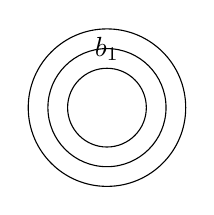
\begin{tikzpicture}
	\draw[color = black] (0,0) circle(0.50);
	\draw[color = black] (0,0) circle(0.75) +(0,0.75) node {$b_1$};
	\draw[color = black] (0,0) circle(1.00);
\end{tikzpicture}
\end{center} 

Þá myndast nýr stafn í hvert sinn, hinsvegar þegar tími líður ferðast
stafninn áfram og er hraði bylgjunar kallaður bylgjuhraði eða
oftar útbreiðsluhraði bylgjunar, s.s. hversu hratt bylgjan breiðir
úr sér. Mælieiningin sem er er notuð er mæld í metrum per sekúndu eða
$\uspeedms$.

Þegar bylgjustafn er bein lína er hægt að ímynda sér sett af línum
sem myndast og ferðast síðan fram á við
\begin{center}
\begin{tikzpicture}
	\draw[color = black] (0,0) -- (0,1) node[above] {$b_1$};
\end{tikzpicture}
\end{center}

\subsection{Bylgjustafn og brot}
Þegar flatur bylgjustafn lendir á littlu gati getur hann umbreyst frá því
að vera flatur stafn yfir í að verða kúlustafn. Í raun er stafninn ennþá
,,flatur'' í fyrri skilgreiningi, bara í stað þess að vilja fara beint
áfram er það styttra að ferðast meðfram bogaferli en að þvinga sig beint
áfram. Ef opið er haft nægilega breitt þá myndast beinn stafn að hluta
til en ef opið er of lítið getur enginn stafn myndast.
\begin{center}
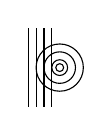
\begin{tikzpicture}
	\draw[color = black] (0,0) -- (0,1);
	\draw[color = black] (0.1,0) -- (0.1,1);
	\draw[color = black] (0.2,0) -- (0.2,1);
	\draw[color = black] (0.3,0) -- (0.3,1);
	\draw[color = black] (0.4,0.5) circle(0.05);
	\draw[color = black] (0.4,0.5) circle(0.1);
	\draw[color = black] (0.4,0.5) circle(0.2);
	\draw[color = black] (0.4,0.5) circle(0.3);
\end{tikzpicture}
\end{center}
til að prufa slíkt í raunveruleikanum er kjörið að prufa slíkt með vatni
í bala. Með því að dýfa littlum pinna í vatnið er hægt að skapa
kúlustafn og með því að dýfa þunnum ferköntuðum hlut í vatn er hægt að
skapa flatbylgjur.

\section{Lögmál Huygens}
Hægt er að nýta lögmál Huygens til að finna bylgjustafn frá við mismunandi
punktbrot og línubrotl.

\section{Ljósbognun}

\section{Samliðun í föstum efnum}
Bylgjur sem ferðast í gegnum efni geta náð að mynda samliðun með reglulegu
millibili. Þá er hægt að ímynda sér að bylgjustafn sem lendir þvert á
sett af atómum og myndar kúlubylgju í stað fyrir þverbylgju. Frá hverju
atómi kemur kúlubylgja sem myndar gagnlega og eyðandi samliðun við hin
atómin. Sem stærð er hægt að setja það í jöfnuform á hvaða hornum
samliðunum á sér stað. Gagnleg samliðun gerist við
\begin{align}
	\unumbern \uwavelength_\unumbern &= \ulengthd \sin{ \varphi_\unumbern } 
\end{align}
fyrir eyðandi samliðun þá er jafan
\begin{align}
	\frac{\unumbern}{2} \uwavelength_\unumbern &= \ulengthd \sin{ \phi_\unumbern } 
\end{align}
sönnunin á þessu er áhugaverð blanda af hornafræði og bylgjuútbreiðslu.
Fyrir gagnlega samliðun þá er bara hægt að tala um algjöra samliðun þegar
bylgjutopparnir eru eina bylgjulengd frá hvor öðrum.
\\
\begin{center}
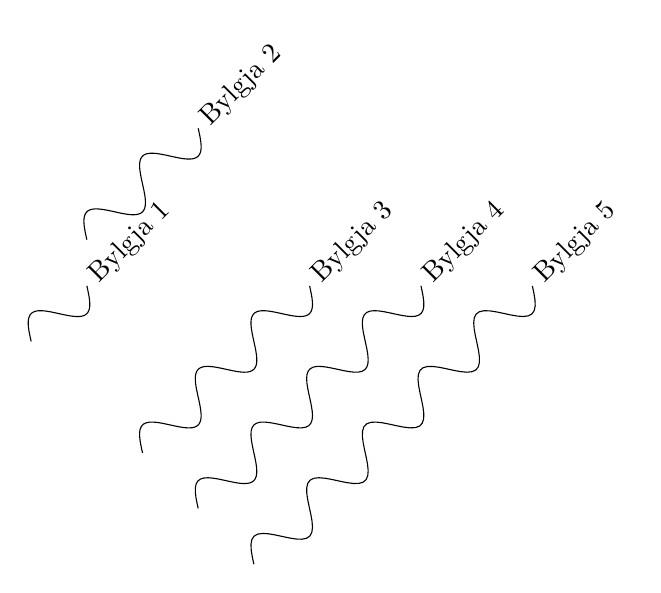
\begin{tikzpicture}[
	force/.style={>=latex,draw=blue,fill=blue, very thick},
	forcecomp/.style={>=latex,draw=blue, densely dashed, fill=blue},
	axis/.style={densely dashed,gray,font=\small},
	m/.style={rectangle,draw=black,fill=gray,minimum size=0.3cm,thin},
	M/.style={rectangle,draw,fill=lightgray,minimum size=0.3cm,thin},
	scale=1,
	domain=0:{3.141*2}
	]
	\draw[color = black, samples=100, domain=0:{3.141*2*1}, rotate=45] 
		plot({\x/3.141/2},{0.25*sin(\x r)}) node[right, rotate=45] {Bylgja 1};
	\draw[color = black, samples=100, domain=0:{3.141*2*2}, yshift=2cm, rotate=45] 
		{plot(\x/3.141/2,{0.25*sin(\x r)-1.0})} node[right, rotate=45] {Bylgja 2};
	\draw[color = black, samples=100, domain=0:{3.141*2*3}, rotate=45] 
		plot(\x/3.141/2,{0.25*sin(\x r)-2.0}) node[right, rotate=45] {Bylgja 3};
	\draw[color = black, samples=100, domain=0:{3.141*2*4}, rotate=45] 
		plot(\x/3.141/2,{0.25*sin(\x r)-3.0}) node[right, rotate=45] {Bylgja 4};
	\draw[color = black, samples=100, domain=0:{3.141*2*5}, rotate=45] 
		plot(\x/3.141/2,{0.25*sin(\x r)-4.0}) node[right, rotate=45] {Bylgja 5};
\end{tikzpicture}
\end{center}

\section{Lögmál Braggs}
% add thin diffraction
Þegar bylgjustafn (oft röntgen geislar) lendir á atómum myndast gagnleg samliðun sem er eins og 
hefðbundin samliðun, nema hvað það kemur auka tala með sem tvölfaldar
bylgjulengdina á stafninum. Úr því kemur lögmál Braggs sem er einungis hægt
að nota fyrir þunnar himnur.
\begin{equation}
	\unumbern \uwavelength_\unumbern = 2\ulengthd \sin{ \varphi_\unumbern }
\end{equation}
til að sanna þetta lögmál er hægt að búa til teikningu sem sýnir hvaðan
þessi tvöföldun kemur \\
\begin{center}
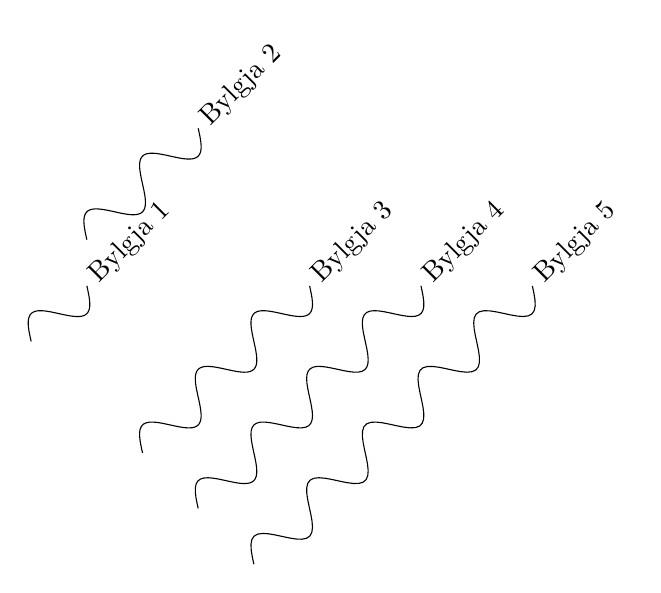
\begin{tikzpicture}[
	force/.style={>=latex,draw=blue,fill=blue, very thick},
	forcecomp/.style={>=latex,draw=blue, densely dashed, fill=blue},
	axis/.style={densely dashed,gray,font=\small},
	m/.style={rectangle,draw=black,fill=gray,minimum size=0.3cm,thin},
	M/.style={rectangle,draw,fill=lightgray,minimum size=0.3cm,thin},
	scale=1,
	domain=0:{3.141*2}
	]
	\draw[color = black, samples=100, domain=0:{3.141*2*1}, rotate=45] 
		plot({\x/3.141/2},{0.25*sin(\x r)}) node[right, rotate=45] {Bylgja 1};
	\draw[color = black, samples=100, domain=0:{3.141*2*2}, yshift=2cm, rotate=45] 
		{plot(\x/3.141/2,{0.25*sin(\x r)-1.0})} node[right, rotate=45] {Bylgja 2};
	\draw[color = black, samples=100, domain=0:{3.141*2*3}, rotate=45] 
		plot(\x/3.141/2,{0.25*sin(\x r)-2.0}) node[right, rotate=45] {Bylgja 3};
	\draw[color = black, samples=100, domain=0:{3.141*2*4}, rotate=45] 
		plot(\x/3.141/2,{0.25*sin(\x r)-3.0}) node[right, rotate=45] {Bylgja 4};
	\draw[color = black, samples=100, domain=0:{3.141*2*5}, rotate=45] 
		plot(\x/3.141/2,{0.25*sin(\x r)-4.0}) node[right, rotate=45] {Bylgja 5};
\end{tikzpicture}
\end{center}


%\input{sections/chap_standing_waves}

% 
% Thermodynamics
% 

\part{Varmafræði}
% 
% A container for thermodynamics
% 

% Chap temperature
\chapter{Hiti}
Hitastig er lýsing á hreyfingu atóma, eftir því sem hitastigið er hærra þá er
hreyfingin meiri. Í daglegu tali er oftast notast við Celcíus skalann ($\udegcent$),
hins vegar finnast margar leiðir til að kvaðra hita. Hiti er mælieining sem er
miðuð við einhvern kvaðra, t.d. er Celcíus kvarðinn miðaður við bræðslumarks
vatns. Farenheit kvarðinn er miðaður við jafnvægisblöndu af þrem efnum,
vatni, ís og ammóníumklóri. Kelvinn kvarðinn miðast við meðalhreyfiorku atóma
og núll hreyfiorka er jafngildi núll hita. Einingin fyrir Kelvin er $\ukelvin$.
Til að breyta kelvin í gráður celcíus
\begin{equation}
	\utemperature_\text{celcíus} = \utemperature_\text{kelvin} - 273,15
\end{equation}
og til að breyta gráður celcíus í kelvin
\begin{equation}
	\utemperature_\text{kelvin} = \utemperature_\text{celcíus} + 273,15
\end{equation}
sem er hægt að nýta á marga máta. Það ætti að vera venja að alltaf vinna með
SI-einingar. Fyrir flestar jöfnur er það krafa að vinna með Kelvin skalann,
undanteikningin er þegar breyting á hitastigi á sér stað. Fyrir Kelvin og Celcíus
þá er $\Delta\utemperature_\text{kelvin} = \Delta\utemperature_\text{celcíus}$.

\begin{formalexample}
Breyttu $92 \udegcent$ í kelvin og breyttu $310 \ukelvin$ í gráður celcíus.
\\[4 ex]
Þá er
\[
	92 \udegcent = (92+273,15) \ukelvin = 365 \ukelvin
\]
og
\[
	310 \ukelvin = (310-273,15) \udegcent = 36,8 \udegcent \approx 37 \udegcent
\]

\end{formalexample}
\chapter{Gasjafnan}\label{section:thermodynamics:idealgas}
Gas getur fundist í mörgum ástöndum, þá er gas sem er hagar sér eins og það er
samsett af kúlum sem hafa næga hreyfiorku til að yfirvinna bindisorkuna
sem gasatómin geta haft sín á milli. Þá kallast slíkt gas, \emph{kjörgas}
þar sem það er bara stjórnað af hitastigi, þrýstingi og rúmmáli. Þá skiptir
ekki máli hvort að um er að ræða atóm eða sameindir, svo lengi sem eigin
hreyfiorka markvert stærri en bindiorka á milli gaseindana. Þá er gasjafnan
gefin við
\begin{align}
	\upressure \uvolume &= \unumberN \uboltzmann \utemperature
\end{align}
líka er til önnur útgáfa sem mikið notuð í efnafræði
\begin{align}
	\upressure \uvolume &= \unumbern \ugasconstant \utemperature
\end{align}
Bæði tilvikin eru gaslögmálið fyrir kjörgas, þess ber að merkja að
þrýstingur margfaldaður með rúmmáli hefur sömu einingu og orka.
Reyndar er þetta orkan sem kjörgas hefur í samræmi við hitastigið sem gasið
finnst við. Fyrri jafnan skoðar orkuna á hverri eind sem finnst í gasinu á meðan
seinni skoðar magnið af orku sem finnst í einu móli af kjörgasi.
Þá er fasti Boltzmanns $\uboltzmann = \ugasconstantjk$ og gasfastinn
$\ugasconstant = \ugasconstantjkm$. 

\begin{formalexample}
	Ílát sem er með rúmmálið $0,1 \, \si{\metre\cubed}$ inniheldur 
	$\num{8,5} \, \si{\mole}$ af
	kjörgasi, þrýstingurinn í ílátinu er 
	$\num{2e5} \, \si{\pascal}$. Hvert er
	hitastigið í flöskunni?
	\\[4 ex]
	Hægt er að nota gasjöfuna með gasfastanum til að einangra hitan úr
	kjörgasjöfnunni
	\begin{align*}
		\num{2e5} \, \si{\pascal} \times 0,1 \, \si{\metre\cubed}
			&= \num{8,5} \, \si{\mole} \times 
				\ugasconstantjkm \times \utemperature 
			&& \Leftrightarrow \\
		\utemperature  &= \frac{ \num{2e5} \, \si{\pascal} \times 0,1 \, 
				\si{\metre\cubed} }
			{ \num{8,5} \, \si{\mole} \times \ugasconstantjkm } \\
		&= 283 \si{\kelvin} \\
		&= 10 \si{\celsius}
	\end{align*}
	sem þýðir að hitastigið er að meðaltali í ílátinu $10 \si{\celsius}$
\end{formalexample}
Þegar Boltzmanns fastinn er
notaður er talað um meðalorku per atóm í kjörgasi. 
Hægt er að lesa fastan $\uboltzmann = \ugasconstantjk$ sem 
$1,38 \si{\joule}$ af orku á hvert einasta atóm í gasinu fyrir hvert Kelvin.
\begin{formalexample}
	Loftþéttur stálkassi inniheldur $\num{5e24}$ atóm, þrýstingurinn í kassanum
	er mældur til að vera $\num{3e5} \, \si{\pascal}$ og hitastigið er mælt til
	að vera $\num{320} \, \si{\kelvin}$. Áætlaðu að gasið í kassanum sé
	kjörgas, finndu rúmmál kassans.
	\\[4 ex]
	Hægt er að nota gasjöfuna til að finna rúmmálið á kassanum með
	\begin{align*}
		\num{3e5} \, \si{\pascal} \times \uvolume
			&= \num{5e24} \times \ugasconstantjk \times \num{320} \, \si{\kelvin}
			&& \Leftrightarrow \\
		\uvolume
			&= \frac{ 
				\num{5e24} \times \ugasconstantjk \times 
				\num{320} \, \si{\kelvin}
				}{
				\num{3e5} \, \si{\pascal}
				}
			\\
			&= \frac{ 
				\num{2.2e4} \, \si{\joule}
				}{
				\num{3e5} \, \si{\pascal}
				}
			\\
			&= \num{0.073} \, \si{\metre\cubed} \\
			&= \num{73} \, \si{\deci\metre\cubed} \\
			&= \num{73} \, \si{\liter}
	\end{align*}
	Sem þýðir að kassinn fyllir $\num{73} \, \si{\liter}$ af rúmmáli. Hins vegar
	er hægt að finna út afhverju $\si{\joule\per\pascal} = \si{\metre\cubed}$,
	þegar við skoðum eininguna $\si{\joule} = \si{\newton\metre}$ og eininguna
	$\si{\pascal} = \si{\newton\per\metre\squared}$ sem gefur
	\begin{align*}
		\frac{\si{\joule}}{\si{\pascal}} 
			&= 
			\frac{\si{\cancel\newton\metre}}{
				\si{\cancel\newton\per\metre\squared}}
			= 
			\frac{\si{\metre}}{
				\si{\per\metre\squared}}
			= 
			\si{\metre\cubed}
	\end{align*}
\end{formalexample}
Það gildir líka fyrir gaslögmálið að orkan sem gasið hefur dreifist jafn í gegnum
lokað kerfi. Ef rúmmál, hiti eða þrýstingur breytist í lokuðu kerfi er orkan
óbreytt, sem þýðir að hægt er að setja
\begin{align}
	\frac{\upressure_1 \uvolume_1}{\utemperature_1}
		= \unumberN \uboltzmann
		= \unumbern \ugasconstant
		= \frac{\upressure_2 \uvolume_2}{\utemperature_2}
\end{align}
Ef tvö (eða fleiri) kerfi eru tengd saman þá hækkar orkan ekki en hins vegar 
breytist þrýstingur, rúmmál eða hitastig þegar gasið jafnast út. Eitthvað
af stærðunum sem stýra gildunum verða breytast annars hverfur orkan úr
kerfinu!

% heat
% Chap angular motion
\chapter{Varmarýmd}
Þegar hitamismunur á sér stað þá mun heitari hluturinn reyna lækka hitastigið
sitt og kaldari hluturinn mun reyna hækka hitastigið sitt. Það sem gerist er
að orka færist á milli hlutana og sú orka hefur nafnið varmi.

Varmi er orka, en er nánar tiltekið orka sem tengist hitastigi hluta. Því er
varmaflæði líka orkuflæði, hlutir geta gefið frá sér varma og tekið til
sín varma. S.s. það er geta sem hlutir hafa mismunandi mæli.

Varmarýmd er stærð táknar magnið af orku fyrir hvert kelvin~\footnote{Hægt 
líka að segja hluturinn rúmar orku á hverja kelvin breytingu} 
sem hlutur breytir hita sínum. Í jöfnuformi þá er varmarýmd
\begin{equation}
	\uheatcapacity = \frac{\uthermaleng}{\Delta \utemperature}
\end{equation}
síðan er hægt að mæla varmarýmd hluta með að þekkja magnið af orku sem er notað
til að hita hlutinn upp. Einingin fyrir varmarýmd er $\uheatcapacityjk$ eða
Joule per Kelvin.

\begin{formalexample}
Ílát er hitað upp með rafhitara sem hefur aflið $2 \ukilo\uwatt$, uþb. $80\%$ af
orku rafhitarns fer í að hita ílátið, eftir að rafhitarinn er búin að vera
í gangi í $2 \umin$ þá er hiti ílátsins búinn að hækka um $20 \ukelvin$.
Hver er varmarýmd ílátsins?
\\[4 ex]
tíminn sem hitarinn er í gangi eru $2 \umin = 120 \usec$ og orkan sem hann lætur
í té er
\[
	\Delta\upotentialu = \upower \Delta\utime 
		= \uEE{2}{3} \uwattjs \cdot 120 \utime
		= 240 \ukilo\ujoule
\]
og af þessari orku, þá er $\uthermaleng = 0,80 \cdot 240 \ukilo\ujoule 
= 192 \ukilo\ujoule$ sem gefur að varmarýmdin er
\begin{align*}
	\uheatcapacity &= \frac{\uthermaleng}{\Delta \utemperature} \\
		&= \frac{\uEE{192}{3} \ujoule}{20 \ukelvin} \\
		&= 9600 \uheatcapacityjk 
\end{align*}
\end{formalexample}

\section{Eðlisvarmi}
Eðlisvarmi er sama hugtak og varmarýmd nema þá er tekið mark á massa hlutsins
sem hefur varmarýmdina. S.s. eðlisvarmi er varmarýmd per kílógramm. Eðlisvarmi er
gefin til að vera
\begin{equation}
	\uspecificheat = \frac{\uthermaleng}{\umass \Delta\utemperature}
\end{equation}
þar sem einingin fyrir eðlisvarma er $\uspecificheatjkgk$. Önnur heppileg
leið til að sýna sömu jöfnu er
\[
	\uthermaleng = \umass \uspecificheat \Delta \utemperature
\]
en þessi jafna er í raun útleitt form af varmarýmd per massa.
\begin{formalexample}
Hversu mikla orku þarf til þess að hita 2 lítra af vatni um $30 \ukelvin$? 
Eðlisvarmi vatns er $4186 \uspecificheatjkgk$.
\\[4 ex]
Varminn sem vatnið tekur við er
\begin{align*}
	\uthermaleng &= \umass \uspecificheat \Delta \utemperature \\
		&= 2 \ukilo\ugramm \cdot 4186 \uspecificheatjkgk \cdot 30 \ukelvin \\
		&= 251 \ukilo\ujoule 
\end{align*}
\end{formalexample}

\section{Gagnleg not af varmarýmd}
Dæmi um nýtingu varmarýmdar er oftast til að finna breytingu í hitastigi hluta
miðað við magnið af orku sem er gefin eða þeginn sem varmi. Það sem er oft góð
hugmynd að áætla er að varmi sem hlutur getur látið frá sér fer allur í hlutinn
sem þiggur. Sem gefur
\[
	\uthermaleng_\text{gefin} = \uthermaleng_\text{þeginn}
\]
til að byrja með virðist þetta ekki vera einstaklega hagnýtt fyrirbæri. Vonin er
að sýna hvernig þetta litla samhengi leggur drög að góðu verkfæri.

\begin{formalexample}
$20 \ugramm$ af ís við bræðslumark er færður í skál með $0,5 \uliter$ af $20 
\udegcent$ heitu vatni. Hvert er lokahitastigið á vatninu með bráðnaða ísnum?
\\[4 ex]
Vatnið sem ísinn er lagður mun tapa varma sem ísinn mun allur nýta, þeas. vatnið
gefur varman sem ísinn þiggur. Bæði bráðnaði ísinn og vatnið munu enda í sama 
lokahitastigi. Orka sem krefst að breyta hitastigi vatnsins er
\begin{align*}
	\uthermaleng_\text{vatn} &= \umass_\text{vatn} \uspecificheat_\text{vatn}\Delta \utemperature_\text{vatn} \\
		&= 0,5 \ukilo\ugramm \cdot 4186 \uspecificheatjkgk \cdot \Delta \utemperature_\text{vatn} \\
		&= 2093 \uheatcapacityjk \cdot \Delta \utemperature_\text{vatn}
\end{align*}
varminn sem ísinn þiggur er
\begin{align*}
	\uthermaleng_\text{ís} &= \ulatentheat \umass_\text{ís} 
		+ \umass_\text{ís} \uspecificheat_\text{vatn}\Delta \utemperature_\text{ís} \\
		&= \uEE{334}{3} \ulatentheatjkg \cdot 0,020 \ukilo\ugramm 
			+ 0,02 \ukilo\ugramm \cdot 4186 \uspecificheatjkgk \cdot \Delta \utemperature_\text{ís} \\
		&= 6680 \ujoule +  83,7 \uheatcapacityjk \cdot \Delta \utemperature_\text{ís}
\end{align*}
þar sem við erum bara taka stærðina af varmanum þá er krafa að hitastigsbreytingar
séu jákvæðar. Við vitum líka að ísinn fer frá $0 \udegcent$ til 
$\utemperature_\text{lok}$ og vatnið fer frá $20 \udegcent$ til $\utemperature_\text{lok}$.
Samanlagt er stærðin hitastigsbreytingu 
$\Delta \utemperature_\text{vatn} + \Delta \utemperature_\text{ís} = 20 \ukelvin$.
Sem þýðir að $\Delta \utemperature_\text{ís} = 20 \ukelvin - \Delta \utemperature_\text{vatn}$
Gefur það að varminn sem ísinn þiggur er
\begin{align*}
	\uthermaleng_\text{ís}  &= 6680 \ujoule +  83,7 \uheatcapacityjk \cdot \Delta \utemperature_\text{ís} \\
		&= 6680 \ujoule +  83,7 \uheatcapacityjk \cdot \left(20 \ukelvin - \Delta \utemperature_\text{vatn} \right)
\end{align*}
þá er hægt að setja að varminn sem vatnið gefur er þegið af ísnum
\begin{align*}
	\uthermaleng_\text{vatn} &=  \uthermaleng_\text{ís} \\
	2093 \uheatcapacityjk \cdot \Delta \utemperature_\text{vatn}
		&= 6680 \ujoule +  83,7 \uheatcapacityjk \cdot 20 \ukelvin - 83,7 \uheatcapacityjk \cdot \Delta \utemperature_\text{vatn}\\
	2093 \uheatcapacityjk \cdot \Delta \utemperature_\text{vatn}
		&= 6680 \ujoule +  1674 \ujoule - 83,7 \uheatcapacityjk \cdot \Delta \utemperature_\text{vatn} \\
	2093 \uheatcapacityjk \cdot \Delta \utemperature_\text{vatn} + 83,7 \uheatcapacityjk \cdot \Delta \utemperature_\text{vatn}
		&= 8354 \ujoule \\
	\left( 2093 \uheatcapacityjk + 83,7 \uheatcapacityjk \right) \Delta \utemperature_\text{vatn}
		&= 8354 \ujoule \\
	\left( 2177 \uheatcapacityjk \right) \Delta \utemperature_\text{vatn}
		&= 8354 \ujoule \\
	\Delta \utemperature_\text{vatn}
		&= \frac{8354 \ujoule}{ 2177 \uheatcapacityjk } \\
		&= 3,84 \ukelvin \approx 3,84 \udegcent
\end{align*}
þá er lokahitastigið fyrir vatnið og ísinn
\[
	\utemperature_\text{loka} = 20 \udegcent - 3,84 \udegcent = 16,2 \udegcent
\]
\end{formalexample}

\section{Varmafærsla}
Þegar það er hitastigsmunur í efni þá leitast hitastigið á öllum stöðum í sama
hitastigið. Þetta þýðir að innri varmi efnisins dreifist jafn um efnið, varmi
hefur ekki tilhneigingu til að halda sér á sama stað ef það er hægt að leita til
lægra hitastigs.
 % Technically heat capacity
%\input{sections/heat_kinetic_theory}
% laws of thermodynamics
%
% The definition of thermodynamic systems
%
\chapter{Varmalögmál}
Þegar varmi færist á milli staða er hægt að tala um lokuð og opin
kerfi, þeas. hvort að orka geti horfið úr kerfinu (opið kerfi).
Útfrá því eru nokkur lögmál kynnt á þeim grundvelli. Dagleg
reynsla segir okkur að hlutir reyna að nálgast hitastigið í
því umhverfinu. Þegar ísmoli er tekinn út í hitann þá bráðnar
hann þar sem ísmolinn móttekur varma frá umhverfinu. Þá er
er talað um jafnvægi sem næst á milli ísmolans og umhverfis.

\section{Núllta lögmál varmafræðinnar}
Í grófum dráttum er það:
\begin{quote}
	Þegar tveir hlutir (A og B) eru í jafnvægi við
	þriðja hlut (C), þá eru hlutir A og B í jafnvægi.
	Jafnvægi er skilgreint sem sama hitstig eða 
	jafnorkuflæði á milli hluta
\end{quote}
Lögmálið beinir athyglinni að því að hlutir með varma munu
ekki leita til þess að færa varma sinn nema kerfið sé í ójafnvægi.

\section{Fyrsta lögmál varmafræðinnar}
Orka í lokuðu kerfi er varðveitt, þá hverfur ekki orka í varmafærslu en í staðinn
fer hún í vinnu af hendi kerfisins. Hins vegar þegar orka bætist inní lokað
kerfi verður samanlögð innri orka kerfisins aukin og einhver hluti af orkunni
fer í annað en að auka innri orkuna (þeas. vinna).
\begin{quote}
	Samanlögð breyting á innri okru kerfisins er summan af viðbættri orku í 
	kerfið og vinnunni sem fer í að bæta orkunni við. Í jöfnuformi fæst
	\begin{align}
		\Delta \upotentialu &= \Delta \uthermaleng + \Delta \uworkw
	\end{align}
\end{quote}
Fyrir lokuð kerfi með engri breytingu er $\Delta \upotentialu = \SI{0}{\J}$. 
\begin{formalexample}
	Kjörgas móttekur $\SI{2.5}{\kJ}$ af orku og vinnan framkvæmd af gasinu
	er $\SI{300}{\J}$, hvað er breytingin í innri orku gasins?
	\\[4 ex]
	Þar sem vinnan er framkvæmd af gasinu þá er það orka sem gasið ætlur frá
	sér. Á sama tíma móttekur gasið orku, það gefur 
	\begin{align*}
		\Delta \upotentialu &= \Delta \uthermaleng + \Delta \uworkw \\
			&= \SI{2500}{\J} - \SI{300}{\J} \\
			&= \SI{2200}{\J}
	\end{align*}
	hækka innri orka kjörgasins um $\SI{2.2}{\kJ}$.
\end{formalexample}

\section{Annað lögmál varmafræðinnar}
Sem afleiðing af núllta og fyrsta lögmálinu, þá verður orka að flæða á 
milli hluta sem ná að komast í jafnvægi. Hins vegar segir annað lögmálið að 
varminn flæðir frá heitari hlutnum til kaldari hlutarins, oft er notuð óreiða 
til að lýsa þessu lögmáli. Lítil óreiða er kostnaðarsamari en mikil óreiða 
(við sama hitastig), það virkar andstætt almennri skynsemi en lítil óreiða 
samsvarar mikilli röðun og sem þarf að viðhalda. Lögmálið er oft skrifað sem
\begin{quote}
	Varmi leitar frá heitari hlut til kaldari hluts.
\end{quote}

\section{Þriðja lögmál varmfræðinnar}
Þegar efni kólnar minnkar óreiða efnis, ef efni er kælt til $0 \, \ukelvin$ þá
mun óreiða nálgast núll. Sem lögmál þá er þetta viðbót við annað lögmálið
til að gera fulla grein fyrir óreiðu.
\begin{quote}
	Efni við núll kelvin hefur núll óreiðu.
\end{quote}
\section{Óreiða}
Allt efni hefur innbyggða orku sem tengist hita stigi efnisins, sé hitastigið
hærra verður orkan hærri. Samtímis er hægt að koma með nýtt hugtak, sem er að
efnið hefur innbyrðis röðun og getur bara haft ákveðið mikið af uppröðunum
af staðsetningu og orku. Fyrst er þetta hugtak mjög sérstakt því óreiða er
eitthvað sem öll efni reyna að hámarka, þá vill efni koma sem mestu ,,óskipulagi''
í umhverfið. Óreiðu er líka hægt að lýsa sem magn af orku sem á eftir að
ná að dreifa sér út almennilega. Það eru talsvert margar myndlíkingar
á óreiðu en það er hægt að lýsa magninu af óreiðu með tölum og
stærðum. Djúp lýsing á óreiðu sem nær alla leið niður á atómskalan krefst
umtalsverðar stærðfræði og því verður ekki meðhöndluð á þann máta. 
Verður stuðst við myndlíkingar til að reyna skapa skilning.


% 
% Electrodynamics
% 

\part{Rafsegulfræði}
% current
\chapter{Straumur}
% Intro to chapter, laws of force
Þegar rafeindir ferðast í leiðurum þá myndast rafstraumur, eða einfaldlega
straumur. Vatnsstraumur er t.d. vatnsmagn á tímaeiningu, oft lýst sem
massi per tímaeingu $\frac{\ukilo\ugramm}{\usec}$. Á svipaðan máta 
er straumur gefinn sem $\frac{\ucoulomb}{\usec}$, þar sem $\ucoulomb$ er
,,magnið'' af rafmagni (svipar til massa). Einingin sem er notuð fyrir
straum er Amperé\footnote{Fengið frá
\url{http://en.wikipedia.org/wiki/Andr\%C3\%A9-Marie_Amp\%C3\%A8re}}
($\uamper$) sem er það sama og að segja $\uampercs$.
\marginpar{
	\begin{center}
	\includegraphics*[
		width= \marginparwidth
		]{./pictures/Ampere_Andre_1825.eps}
	\end{center}
	André-Marie Amperé(1775-186) var franskur 
	vísindamaður sem gerði tilraunir með
	rafkrafta í rafmagnsleiðurum.
	}


\section{Hleðsla og rafeindir}
% Examples of size, direction
Hleðsla sem stærð er eitthvað sem sumar eindir búa yfir sem eiginleiki,
þetta er svipað og sumar eindir hafa massa (t.d. $\ukilo\ugramm$). Það
eru ekki allar eindir sem búa yfir massa, ljós er massalaus eind á meðan
rafeindin hefur massa. Hleðsla er ,,form'' af massa, eitthvað sem sumar
eindir hafa og aðrar ekki, í þessum kafla eru bara rafeindir, jáeindir
og róteindir með hleðslu. Það eru talsvert fleiri eindir sem bera hleðslu
á sama máta og það eru til talsvert fleiri eindir sem hafa massa. Þá
er \emph{grunnhleðsla} hugtak sem er viðmiðunarpunktur af hleðslu.
Grunnhleðslan er
\begin{align}
	\uelementcharge &= \uEE{1,602}{-19} \ucoulomb
\end{align}
sem er jafn stór og hleðslan og ein rafeind, jáeind eða róteind hefur.
\begin{table}[!h]
	\begin{center}
	\begin{tabular}{ccc}
	\toprule
	Heiti & Tákn & Hleðsla \\
	\midrule
	Rafeind  & $\uelectron$ & $-\uelementcharge$ \\
	Jáeind  & $\upositron$ & $+\uelementcharge$ \\
	Róteind  & $\uproton$ & $+\uelementcharge$ \\
	\bottomrule
	\end{tabular}
	\end{center}
	\caption{Yfirlit yfir hleðslu frumeinda}
\end{table}
\begin{formalexample}
Hvað eru margar rafeindir í einu kúlombi?
\\[4 ex]
Þegar grunnhleðslan per rafeind er
\[
	\uelementcharge = \uEE{1,602}{-19} \frac{\ucoulomb}{\text{rafeind}}
\]
þá er fjöldi rafeinda
\begin{align*}
	\text{fjöldi} =
		\frac{ 1 \ucoulomb}{\uEE{1,602}{-19} \frac{\ucoulomb}{\text{rafeind}} }
	= \uEE{6,242}{18} \text{rafeindir}
\end{align*}
sem er talsverður fjöldi rafeinda. Almennt er eitt $\ucoulomb$ fremur stór stærð
af rafeindum en þegar við mælum straum er hún hentugri til en fjöldi rafeinda.
\end{formalexample}

\section{Straumur}
% Current
Straumur er þegar hleðsla (sem geta verið rafeindir) færist á milli staða, færsla
á hleðsu myndar strauminn en annað hugatak sem kallast spenna sér um að ýta
hleðslunni áfram. Til samanburðar er hægt að ímynda sér að hleðsa sé vatn og
þyngdarkrafturinn sé spennan sem togar vatnið áfram. Einingin fyrir straum er
$\uamper$ eða $\uampercs$, SI-einingin er samt $\uamper$ er oftast gefinn upp.
Þá er straumur gefinn við
\begin{align}
	\ucurrenti &= \frac{\Delta\uchargeQ}{\Delta\utime}
\end{align}
þar sem er $\Delta\uchargeQ$ magnið af hleðslu sem hefur fengið færslu á 
tímabilinu $\Delta\utime$.
\begin{formalexample}
Mjög þolinmóður talningsmaður hefur talið að í $1\ugramm$ af kopari eru
$\uEE{1,5}{20}$ rafeindir sem geta fært sig. Hann tengir vír við 
koparinn (undir spennu) og mælir strauminn $5 \umilli\uamper$. Hvað tekur það
langan tíma að færa allar rafeindirnar úr koparinum?
\\[4 ex]
Þegar grunnhleðslan per rafeind er
\[
	\uelementcharge = \uEE{1,602}{-19} \frac{\ucoulomb}{\text{rafeind}}
\]
þá er heildarhleðslan
\begin{align*}
	\Delta\uchargeQ &=
		\uEE{1,602}{-19} \frac{\ucoulomb}{\text{rafeind}} \cdot
		\uEE{1,5}{20} \text{rafeindir}
	&= 24,03 \ucoulomb
\end{align*}
hægt er að umskrifa straumjöfnuna til að vera
\begin{align*}
	\Delta\utime &= \frac{\Delta\uchargeQ}{\ucurrenti}
		&= \frac{24,03 \ucoulomb}{\uEE{5}{-3} \uamper}
		&= 4806 \usec = 80 \umin
\end{align*}
ef spennan yrði aukin myndi tíminn minnka, samsvarar að nota stærri kraft til að
hreyfa rafeindirnar.
\end{formalexample}

% electric force
\chapter{Rafkraftur}
% Intro to chapter, laws of force
Á sambærilegan máta og þyngdarafl þá eru hlutir sem hafa hleðslu munu verka
með krafti á hvort annað, stærð kraftsins er í samræmi við magn hleðslu
hlutarins. Hleðsla er einfaldlega eiginleiki sem efni hefur á sama máta
og efni getur haft eiginleikan massa. Rafeindar hafa bæði massa og
hleðslu og því getur þyngdarkraftur og rafkraftur verkað á rafeindina.

Eindir eða hlutir sem hafa enga hleðslu verða því ekki fyrir áhrifum
rafkrafts, niftendir eru gott dæmi um slíkt, hún hefur massa og enga
\emph{ytri hleðslu}\footnote{Niftendir eru samsettar úr kvörkum sem
hafa hleðslu en samanlagt verður hleðslan núll á nifteindinni}. Róteindir
hafa hins vegar andstæða hleðslu við rafeindir og hafa líka mun
meiri massa.

Tilraunir sýna að neikvæð hleðsla (rafendir) dregst að jákvæðri hleðslu
(róteindir) með aðdráttarkrafti, hins vegar mun neikvæð hleðsla valda 
fráhrindikrafti á aðra neikvæða hleðslu. Tvær jákvæðar hleðslur valda 
sömuleiðis fráhrindikrafti á hvor aðra. Lögmálið sem lýsir kraftinum er
\begin{align}
	\uforce_\text{raf} &= \uconstk \frac{\uchargeq \uchargeQ}{\ulengthr^2}
\end{align}
þar sem $\uchargeq$ og $\uchargeQ$ er stærð hleðslanna sem verka á
hvor aðra og $\ulengthr$ er lengdin á milli hleðsla. Fastinn $\uconstk$ er gefinn
til að vera $\ucoulombconstantenmc$ og er kallaður fasti Coulombs. Álíka ber
fyrrnefnt lögmál, kraftalögmál Coulombs%
\footnote{Fengið af 
\url{http://en.wikipedia.org/wiki/Charles-Augustin_de_Coulomb}}. %
\marginpar{ 
	\begin{center}
	\includegraphics*[
		width= \marginparwidth
		]{./pictures/Charles_de_coulomb.eps}
	\end{center}
	Charles-Augustin de Coulomb var franskur eðlisfræðingur (f. 1736
	-d. 1806) sem kom með skilgreininguna á rafkrafti sem lögmál. 
	}

Fasti Coulombs þjónar sama tilgangi og þyngdarfastinn í þyngdarlögmáli Newtons,
sem er krafturinn sem massar verkar á hvorn annan í ferningslengd%
\footnote{Ferningslengd er sama og að segja lengd í öðru veldi 
	($\si{\metre\squared}$). Svipað er ferningsmassi gefinn sem 
	$\si{\kilo\gram\squared}$.
	}
per
ferningsmassa. Á svipaðan máta er fasti Coulombs tengdur við rafkraftinn sem 
hleðslur verka á hvor aðra í ferningslengd per ferningshleðslu. Mikilvægt er að
muna 

\section{Stefna rafkrafta}
Rafkraftur hefur stefnu, nánar tiltekið þá er stefna rafkrafts samsíða beinni
línu á milli hleðsla. Formerki hleðslna stýra stefnu krafts og er neikvætt
formerki oftast meint sem aðdráttarkraftur og jákvætt formerki meint sem
fráhrindikraftur. Gefin eru nokkrar myndir um hvernig rafkraftur hanga sér miðað
við hleðslu:
\begin{center}
	\begin{tikzpicture}[
		scale=1.0, 
		place/.style={circle,draw=black,fill=blue!20,thick,
		inner sep=0pt,minimum size=16mm},
		force/.style={>=latex,draw=blue,fill=blue, very thick, ->}
		]
		\node[place] (m1) at (-2.5,0) {Massi 1};
		\node[place] (m2) at (2.5,0) {Massi 2};
		\draw[force] (m1.east) -- ++(1,0) node[above] {$\uforce_\text{raf}$};
		\draw[force] (m2.west) -- ++(-1,0) node[above] {$\uforce_\text{raf}$};
		\node[below, fill=blue!10] (t) at (m1.south) { Jákvæð hleðsla $+$};
		\node[below, fill=blue!10] (t) at (m2.south) { Neikvæð hleðsla $-$};
	\end{tikzpicture}
\end{center}
\begin{center}
	\begin{tikzpicture}[
		scale=1.0, 
		place/.style={circle,draw=black,fill=blue!20,thick,
		inner sep=0pt,minimum size=16mm},
		force/.style={>=latex,draw=blue,fill=blue, very thick, ->}
		]
		\node[place] (m1) at (-2.5,0) {Massi 1};
		\node[place] (m2) at (2.5,0) {Massi 2};
		\draw[force] (m2.east) -- ++(1,0) node[above] {$\uforce_\text{raf}$};
		\draw[force] (m1.west) -- ++(-1,0) node[above] {$\uforce_\text{raf}$};
		\node[below, fill=blue!10] (t) at (m1.south) { Neikvæð hleðsla $-$};
		\node[below, fill=blue!10] (t) at (m2.south) { Neikvæð hleðsla $-$};
	\end{tikzpicture}
\end{center}
\begin{center}
	\begin{tikzpicture}[
		scale=1.0, 
		place/.style={circle,draw=black,fill=blue!20,thick,
		inner sep=0pt,minimum size=16mm},
		force/.style={>=latex,draw=blue,fill=blue, very thick, ->}
		]
		\node[place] (m1) at (-2.5,0) {Massi 1};
		\node[place] (m2) at (2.5,0) {Massi 2};
		\draw[force] (m2.east) -- ++(1,0) node[above] {$\uforce_\text{raf}$};
		\draw[force] (m1.west) -- ++(-1,0) node[above] {$\uforce_\text{raf}$};
		\node[below, fill=blue!10] (t) at (m1.south) { Jákvæð hleðsla $+$};
		\node[below, fill=blue!10] (t) at (m2.south) { Jákvæð hleðsla $+$};
	\end{tikzpicture}
\end{center}
þá ber að nefna að stefna og stærð eru aðskildar stærðir, stefna kraftins er háð
formerkjum hleðsla en hins vegar er stærð kraftsins gefin við lögmál Coulombs.
Almennt er nauðsyn að taka tillit stefnu rafkrafta þar sem hleðslur hafa títt
mismunandi hleðslu eða sömu hleðslu.

\begin{formalexample}
	Tvær rafeindir með hleðsluna $\num{-1.602e-19} \, \si{\coulomb}$ liggja
	$\num{20} \, \si{\nano\metre}$ frá hvor annari. Hver er stærð og stefna
	rafkraftsins sem verkar rafeindirnar?
	\\[4 ex]
	Fyrst þarf að reikna stærð rafkraftsins
	\begin{align*}
		\uforce_\text{raf}
		&=
		\uconstk \frac{\uchargeq \uchargeQ}{\ulengthr^2} \\
		&= \ucoulombconstantenmc
		\frac{(\num{-1.602e-19} \, \si{\coulomb}) 
			\times (\num{-1.602e-19} \, \si{\coulomb})
		}{\left( \num{20e-9} \, \si{\metre} \right)^2} \\
		&= \ucoulombconstantenmc
		\frac{\num{2.5664e-38} \, \si{\coulomb\squared} 
			}{\num{4e-16} \, \si{\metre\squared}} \\
		&= \num{5.77e-13} \, \si{\newton}
	\end{align*}
	þar sem formerkið er jákvætt þýðir að það er fráhrindikraftur á milli
	rafeindanna.
	\begin{center}
		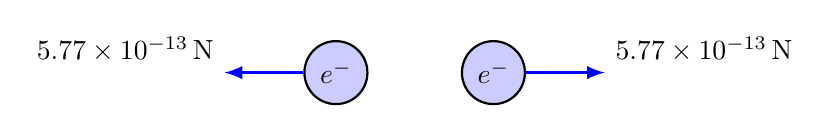
\begin{tikzpicture}[
			scale=1.0, 
			place/.style={circle,draw=black,fill=blue!20,thick,
			inner sep=0pt,minimum size=8mm},
			force/.style={>=latex,draw=blue,fill=blue, very thick, ->}
			]
			\node[place] (m1) at (-1,0) {$e^-$};
			\node[place] (m2) at (1,0)  {$e^-$};
			\draw[force] (m2.east) -- ++(1,0) node[above right] 
				{$\num{5.77e-13} \, \si{\newton}$};
			\draw[force] (m1.west) -- ++(-1,0) node[above left] 
				{$\num{5.77e-13} \, \si{\newton}$};
		\end{tikzpicture}
	\end{center}
	Þá stefnir krafturinn frá sitt hvorri rafeind og með jafnstórri stærð.
\end{formalexample}
\begin{formalexample}
	Hlutur með punkthleðsluna $\num{5} \, \si{\nano\coulomb}$ og
	rafeind liggur í óþekktri vegalengd frá rafeindinni. Hins vegar
	upplifir rafeindin kraftinn $\num{-3} \si{\micro\newton}$.
	\begin{center}
		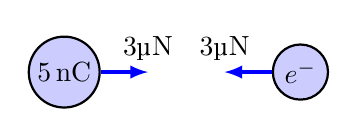
\begin{tikzpicture}[
			scale=1.0, 
			place/.style={circle,draw=black,fill=blue!20,thick,
			inner sep=0pt,minimum size=9mm},
			force/.style={>=latex,draw=blue,fill=blue, very thick, ->}
			]
			\node[place] (m1) at (-1.5,0) {$\num{5} \, \si{\nano\coulomb}$};
			\node[place, minimum size=7mm] (m2) at (1.5,0)  {$e^-$};
			\draw[force] (m1.east) -- ++(0.6,0) node[above] 
				{$\num{3} \si{\micro\newton}$};
			\draw[force] (m2.west) -- ++(-0.6,0) node[above] 
				{$\num{3} \si{\micro\newton}$};
		\end{tikzpicture}
	\end{center}
	Finndu óþekktu vegalengdina á milli hleðslanna.
	\\[4 ex]
	Hægt er að umskrifa lögmál Coulombs sem
	\begin{align*}
		\uforce_\text{raf}
		&=
		\uconstk \frac{\uchargeq \uchargeQ}{\ulengthr^2} && \Leftrightarrow \\
		\ulengthr^2
		&=
		\uconstk \frac{\uchargeq \uchargeQ}{\uforce_\text{raf}} 
		&& \Leftrightarrow \\
		\ulengthr
		&=
		\pm \sqrt{ \uconstk \frac{\uchargeq \uchargeQ}{\uforce_\text{raf}} }
		\\
	\end{align*}
	neikvæða formerkið við rótina hefur ekki þýðingu sem lengd og því er
	það ekki notað. Þetta gefur við innsetningu
	\begin{align*}
		\ulengthr
		&=
		\sqrt{ 
			\ucoulombconstantenmc 
			\frac{ (\num{5e-9} \, \si{\coulomb}) 
				\times (\num{-1.602e-19} \, \si{\coulomb})
				}{\num{-3e-6} \si{\newton}} 
			}
		\\
		&=
		\sqrt{ 
			\num{2.3998e-12} \si{\metre\squared}
			} \\
		&=
		\num{1.55e-6} \si{\metre}
	\end{align*}
	sem þýðir að bilið á milli hleðslunnar og rafeindarinnar er
	$\num{1.55} \si{\micro\metre}$.
\end{formalexample}

\section{Superposition hleðsla}
\todo{Finna íslenskt orð fyrir superposition}% Charge
Hægt er að leggja saman kraftinn á hleðslur, þá geta margar hleðslu verkað á
eina hleðslu. Sem dæmi er hægt að skoða kraftinn sem verkar á eina hleðslu
þegar tvær hleðslur eru lagðar sitthvorum megin við hana.
\begin{center}
	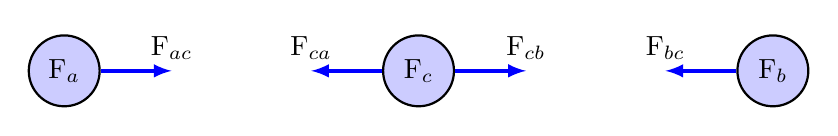
\begin{tikzpicture}[
		scale=3.0, 
		place/.style={circle,draw=black,fill=blue!20,thick,
		inner sep=0pt,minimum size=9mm},
		force/.style={>=latex,draw=blue,fill=blue, very thick, ->}
		]
		\node[place, minimum size=9mm] (m1) at (-1.5,0) {$\uforce_a$};
		\node[place, minimum size=9mm] (m2) at (1.5,0)  {$\uforce_b$};
		\node[place, minimum size=9mm] (m3) at (0,0)  {$\uforce_c$};
		\draw[force] (m1.east) -- ++(0.3,0) node[above] 
			{$\uforce_{ac}$};
		\draw[force] (m3.west) -- ++(-0.3,0) node[above] 
			{$\uforce_{ca}$};
		\draw[force] (m3.east) -- ++(0.3,0) node[above] 
			{$\uforce_{cb}$};
		\draw[force] (m2.west) -- ++(-0.3,0) node[above] 
			{$\uforce_{bc}$};
	\end{tikzpicture}
\end{center}
þá er samanlagður kraftur sem verkar á miðju hleðsluna er þá
\begin{align*}
	\uforce_\text{heild, c} &= \uforce_{ca} + \uforce_{cb}
\end{align*}
hins vegar ef það er skoðað nánar, þá heildarkrafturinn sem verkar á
allt kerfið núll. Sem virkar dálítið sérstakt nema hvað báðar hleðslurnar
verka með jafnstórum og gagnstæðum kröftum. Þá leiðir af sér að
þriðja lögmál Newtons myndar heildkraftinn núll ef enginn
utanaðkomandi kraftur verkar á kerfið þrátt fyrir innri gagnkrafta.
\begin{formalexample}
	Þrjár hleðslur liggja á beinni línu, hver er krafturinn sem verkar
	á hleðsluna C af völdum A og B?
	\begin{center}
		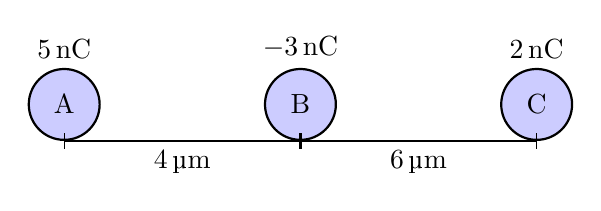
\begin{tikzpicture}[
			scale=2.0, 
			place/.style={circle,draw=black,fill=blue!20,thick,
			inner sep=0pt,minimum size=9mm},
			force/.style={>=latex,draw=blue,fill=blue, very thick, ->}
			]
			\node[place, minimum size=9mm] (m1) at (-1.5,0) {A};
			\node[place, minimum size=9mm] (m2) at (0,0)    {B};
			\node[place, minimum size=9mm] (m3) at (1.5,0)  {C};
			\draw[] (m1.north) node[above] 
				{$\SI{5}{\nano\coulomb}$};
			\draw[] (m2.north) node[above] 
				{$\SI{-3}{\nano\coulomb}$};
			\draw[] (m3.north) node[above] 
				{$\SI{2}{\nano\coulomb}$};
			\draw[|-|] (m1.south) -- (m2.south) node[pos=0.5, below] 
				{$\SI{4}{\micro\meter}$};
			\draw[|-|] (m2.south) -- (m3.south) node[pos=0.5, below] 
				{$\SI{6}{\micro\meter}$};
		\end{tikzpicture}
	\end{center}
	.
	\\[4 ex]
	Þar sem við erum með bæði jákvæðar og neikvæðar hleðslur er nauðsynlegt
	að huga að stefnu rafkraftana sem verka á hleðslu C. Við veljum að jákvæð
	kraftstefna er til hægri að vana. Fyrst er krafturinn
	á mill A og C fráhrindikraftur og samanlagt er vegalengdin á milli A og C
	$\SI{10}{\micro\meter}$. Hleðslurnar ýta hvor annari í burtu með kraftinum
	\begin{align*}
		\uforce_{ca} &=
			\uconstk \frac{\uchargeq_A \uchargeq_C}{\ulengthr_{AC}^2} \\
			&= \ucoulombconstantenmc
				\frac{
					(\SI{5e-9}{\coulomb}) 
					\times (\SI{2e-9}{\coulomb})
					}{\left( \SI{10e-6}{\meter} \right)^2} \\
			&= \SI{898}{\N}
	\end{align*}
	á svipaðan máta er hægt að finna kraftinn á milli B og C, nema hvað það
	er aðdráttarkraftur
	\begin{align*}
		\uforce_{ca} &=
			\uconstk \frac{\uchargeq_B \uchargeq_C}{\ulengthr_{BC}^2} \\
			&= \ucoulombconstantenmc
				\frac{
					(\SI{-3e-9}{\coulomb}) 
					\times (\SI{2e-9}{\coulomb})
					}{\left( \SI{6e-6}{\meter} \right)^2} \\
			&= \SI{-1498}{\N}
	\end{align*}
	þá er heildarkrafturinn á hleðslu C gefinn við 
	\begin{align*}
		\uforce_\text{heild, C} &= \SI{898}{\N} - \SI{1498}{\N} \\
			&= \SI{-600}{\N}
	\end{align*}
	þeas. hleðsla C er dregin í átt að bæði A og B vegna aðdráttarkrafts
	hleðslu B.
\end{formalexample}

\section{Eiginleikar hleðslu}
% Charge
Hleðsla er eiginleiki efnis sem er svipaður og massi, hleðsla er s.s. stærð sem
gefur mælanlegan kraft sem er ekki öðrum stærðum. Tveir helstu kraftarnir sem
koma frá eiginleikum efnis er einmitt rafkraftar og þyngdarkraftar. Hins vegar
eru fleiri kraftar sem efni getur myndað, þar af veikir og sterkir kjarnakraftar.
Hins vegar verða þeir ekki teknir fyrir hér.

\section{Rafsvið}
% Electric fields
Krafturinn sem hleðsla verkar á aðra hleðslu er í beinu samræmi við stærð
upphafshleðslu. Þá er það kraftur á hverja hleðslu einingu sem hægt er að
verka á aðrar hleðslur með. Krafurinn sem verkar á eind með tiltekna hleðslu
$q$ frá hleðslunni $Q$ er hægt að lýsa sem
\begin{align*}
	\uforce &=
			\uconstk \frac{\uchargeq \uchargeQ}{\ulengthr^2}
\end{align*} 
þá þetta kraftur sem verkar á $q$ vegna $Q$. Þá er rafsvið sama og kraftur
á hleðslu, svipað og kraftur per massa í þyngdarsviði. Þá myndi rafsviðið
vera skilgreint sem
\begin{align} \label{equ:electric:efield}
	\uefielde = \frac{ \uforce }{ \uchargeq }
\end{align}
skoðað nánar er hefur þetta eininguna $\si{\N \per \coulomb}$. Það sem ber
að huga, er að prufuhleðslan upplifir kraftinn per hleðslu í rafsviði. Þá
er hægt að ímynda sér að allar aðrar hleðslu en prufuhleðslan mynda rafsvið
sem prufuhleðslan liggur í. Þá myndi rafsviðið sem frá hleðslunni $Q$ sem
verkar á $q$ vera gefið við
\begin{align*}
	\uefielde &= \frac{ \uforce }{ \uchargeq } \\
		&= \uconstk \frac{\uchargeq \uchargeQ}{\uchargeq \ulengthr^2} \\
		&= \uconstk \frac{\uchargeQ}{\ulengthr^2}
\end{align*}
sem sagt rafsviðið sem $q$ upplifir er óháð eigin hleðslu. Þá er stefna
rafsviðs líka mikilvæg, líkt og með krafta þá getum við gefið rafsviði
stefnu. Nánar tiltekið þá getum við ímyndað okkur að jákvæðar hleðslur
hafi rafsvið sem flæðir útfrá hleðslunni, hið gagnstæða myndi vera neikvæð
hleðsla sem tekur á móti rafsviði sem flæðir í átt að neikvæðu hleðslunni.
Þá þarf að skoða hvernig kraftur hagar sér í rafsviði, krafturinn sem
hleðsla myndi upplifa er hægt að umskrifa með hjálp (\ref{equ:electric:efield})
til að vera
\begin{align}
	\uforce &= \uchargeq \uefielde
\end{align}
þá er stefna kraftins háð formerki $\uefielde$ og $\uchargeq$.
\begin{formalexample}
	Eind með hleðsluna $\SI{-5}{\micro\coulomb}$ liggur láréttu
	einsleitu rafsviði með styrkinn $\SI{10}{\N\per\coulomb}$.
	Finndu kraftinn sem hleðslan upplifir í rafsviðinu.
	\begin{center}
		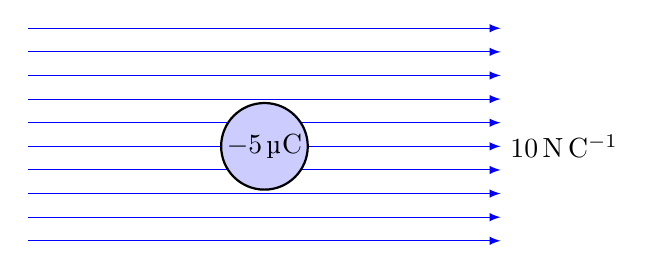
\begin{tikzpicture}[
			scale=3.0, 
			place/.style={circle,draw=black,fill=blue!20,thick,
			inner sep=0pt,minimum size=9mm},
			efield/.style={>=latex,draw=blue,fill=blue!50, thin, ->}
			]
			\foreach \x in {0.1, 0.2, ..., 1.0}
				\draw[efield] (0,\x) -- (2, \x);
			\node[place, minimum size=11mm] (m1) at (1,0.5) 
				{$\SI{-5}{\micro\coulomb}$};
			\draw (2, 0.5) node[right] {$\SI{10}{\N\per\coulomb}$};
		\end{tikzpicture}
	\end{center}
	\vspace{4 ex}
	Þá er mikilvægt að hafa stefnur vel skilgreindar, hérna stefnir
	rafsviðið til hægri og því er valin sem jákvæð stefna. Þegar við
	skoðum stærð kraftsins
	\begin{align*}
		\uforce &= \uefielde \uchargeq \\
			&= \SI{10}{\N\per\coulomb} \times \SI{-5e-6}{\coulomb} \\
			&= \SI{-5e-5}{\N} \\
			&= \SI{-500}{\mN}
	\end{align*}
	sem þýðir að krafturinn verkar gagnstætt stefnu rafsviðsins, myndrænt
	myndi krafturinn vera
	\begin{center}
		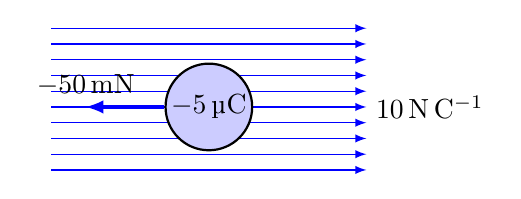
\begin{tikzpicture}[
			scale=2.0, 
			place/.style={circle,draw=black,fill=blue!20,thick,
			inner sep=0pt,minimum size=9mm},
			efield/.style={>=latex,draw=blue,fill=blue!50, thin, ->},
			force/.style={>=latex,draw=blue,fill=blue, very thick, ->}
			]
			\foreach \x in {0.1, 0.2, ..., 1.0}
				\draw[efield] (0,\x) -- (2, \x);
			\node[place, minimum size=11mm] (m1) at (1,0.5) 
				{$\SI{-5}{\micro\coulomb}$};
			\draw (2, 0.5) node[right] {$\SI{10}{\N\per\coulomb}$};
			\draw[force] (m1.west) -- ++(-0.5,0) node[above] {$\SI{-50}{\mN}$};
		\end{tikzpicture}
	\end{center}
\end{formalexample}
rafsviðið sem myndast á milli tveggja hleðsla er venjulega
ekki einsleitt eins og í fyrra dæmi. Þá er rafsviðið sem myndast
á milli tveggja hleðsla gefið \todo{make pretty lines, make tikz
plot the lines} sem
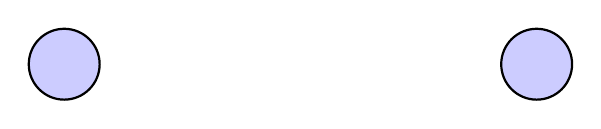
\begin{tikzpicture}[
	scale=3.0, 
	place/.style={circle,draw=black,fill=blue!20,thick,
	inner sep=0pt,minimum size=9mm},
	force/.style={>=latex,draw=blue,fill=blue, very thick, ->},
	]
	\node[place, minimum size=9mm] (m1) at (-1.0,0) {};
	\node[place, minimum size=9mm] (m2) at (1.0,0) {};
\end{tikzpicture}
eftir því hvar rafsviðið á milli hleðslanna er skoðað er það stundum
þéttara en annars. Þéttleikinn á rafsviðinu er í beinu samræmi við
línuþéttleikann á myndinni, því minna bil á milli línanna því stærri
rafsviðsstyrkurinn. Nánar tiltekið, hægt er að lesa myndina á sama
máta og hæðarlínur á kortum, því þéttari sem hæðarlínurnar eru því
meiri breyting er í hæðinni (upp eða niður).
\begin{formalexample}
	Eind með hleðsluna $\SI{5}{\micro\coulomb}$ liggur á beinni línu
	$\SI{2}{\micro\m}$ frá prufhleðslu. Finndu styrk rafsviðsins
	og kraftinn sem prufuhleðslan upplifir ef hún er rafeind.
	\vspace{4 ex}
	
	\noindent Styrkur rafsviðsins sem prufuhleðslan upplifir er einungis háð
	hleðslu eindarinnar, þeas.
	\begin{align*}
	\uefielde
		&= \uconstk \frac{\uchargeQ}{\ulengthr^2} \\
		&= \ucoulombconstantenmc \times
			\frac{\SI{5e-6}{\coulomb}
				}{
				\left( \SI{2e-6}{\m} \right)^2
				} \\
		&= \SI{11.235e15}{\N\per\coulomb} \\
		&= \SI{11.235}{\peta\N\per\coulomb}
	\end{align*}
	sem er ótrúlegur kraftur á hvert Coulomb, ef við skoðum
	kraftinn sem rafeind myndi upplifa í þessu rafsviði þá fæst
	\begin{align*}
		\uforce &= \uefielde \uchargeq \\
			&= \SI{11.235e15}{\N\per\coulomb} \times \SI{-1.602e-19}{\coulomb} \\
			&= \SI{-17.998e-3}{\N} \\
			&= \SI{-18}{\mN}
	\end{align*}
	þá er krafturinn talsvert minni, oft eru rafsvið með gríðarlega styrk en
	stærð kraftsins sem verkar á prufuhleðsluna er í beinu samræmi við eigin
	hleðslu. Þá tvær rafeind myndu upplifa tvöfalda hleðslu.
\end{formalexample}
 

\section{Þyngdar- og rafsvið}
% Similarities between gravity and electric force
Þegar við vinnum hluti sem verða fyrir krafti í fjarlægð, þá er hægt að koma
með samlíkingu á milli áhrifa. Það er svipað mynstur sem bæði rafkraftar
og þyngdarkraftar fylgja. Báðir kraftar hafa öfugt hlutfall við vegalengdina
á milli einda (hleðslur eða massar), þá er almment átt við
\begin{align*}
	F \propto \frac{1}{r^2}
\end{align*}
sem er eins hlutfall fyrir báða krafta. Hins vegar verður lesandi að fara
varlega hvaða ályktanir er hægt að draga af slíku samræmi. Það geti verið
ábending um að það bæði þyngdar- og rafkraftar eru tvö form af sama kraftinum,
nema að þyngdakraftur hefur ekki getað samræmst öðrum kröftum sem heilstætt
líkan fyrir alla krafta. Hægt er að samræma þrjá af fjórum þekktum kröftum
sem eru taldnir stýra alheiminum, nema þyngdarkraftinum, sér í lagi vegna
þess hversu lítill hann er miðað við hina þrjá kraftana.

Þetta er mjög gott dæmi um að fylgni stærða er ekki nauðsynlega vegna
gagnkvæmna afleiðinga, þeas. sem stendur þá lítur út fyrir að
þyngdarkrafturinn er sér á báti.

\section{Fasti couloumbs}
% How it is derived


\chapter{Rafmætti}
% Electric potential

\section{Núll punktur}

\section{Varðveisla orku}
%\input{sections/chap_electric_condensers}

% magnetic field
\chapter{Segulsvið}
% Intro to chapter, laws of force
Segulsvið eru kraftasvið sem eru náteng rafsviðum en hafa samt talsvert
frábrugðna hegðun í samanburði við rafsvið. Segulsvið myndast frá nokkrum gerðum
af málmum, þá nær innri uppbyging efnisins skapa náttúrulegt segulsvið útfrá
hreyfingu rafeinda.

Helsti munurinn á segulsviði og rafsviði er að segulsvið þurfa að flæða í
hringrás. Það leiðir til þess að efni sem er segulmagnað verður að mynda
segulpóla sem eru nefndir norður og suðurpólar. Síðan verkar krafturinn
sem hleðsla upplifir í segulsviði er hornréttur á hreyfiátt hleðslu og
stefnu segulsviðs.

Helsta einingin sem er notuð er Tesla eða $\si{\tesla}$. 
\section{Lögmál Lorentz}
% Examples of size, direction
\marginpar{
	Lorentz er ekki talinn hafa fundið Lögmál Lorentz en hann var sá fyrsti til
	finna skýra stærðfræðilega lýsingu á eiginleikum lögmálsins.
	}
Krafturinn sem hleðsla upplifir er gefinn við krossfeldið á milli hreyfistefnu
og segulsviðs, þá er nauðsynlegt að beita vigrum til að finna kraftstefnu.
Þá eru venslin sem mynda kraftinn gefinn við
\begin{align}
	\vec{\uforce} 
		&= \uchargeq \left( \vec{\uspeed} 
			\times \vec{\umfieldb}  \right)
\end{align}
það er ekki augljóst hvaða afleiðingar þetta hefur fyrir kraftinn sem verkar
á hleðsluna. Þá þarf að vinna úr dæmum með krossfeldum, sem geta verið fremur
ruglingsleg. Krafturinn, hraðinn og segulsviðið er þá gefið við
\begin{align*}
	\vec{\uforce} &= 
		\left( 
		\begin{array}{c} 
			\uforce_\ulengthx \\
			\uforce_\ulengthy \\
			\uforce_\ulengthz \\
		\end{array} 
		\right) \\
	\vec{\uspeed} &= 
		\left( 
		\begin{array}{c} 
			\uspeed_\ulengthx \\
			\uspeed_\ulengthy \\
			\uspeed_\ulengthz \\
		\end{array} 
		\right) \\
	\vec{\umfieldb} &= 
		\left( 
		\begin{array}{c} 
			\umfieldb_\ulengthx \\
			\umfieldb_\ulengthy \\
			\umfieldb_\ulengthz \\
		\end{array} 
		\right) \\
\end{align*}
þar sem $\uforce_\ulengthx$ táknar stærðkraftsins meðfram x-ás. Dæmi teikningu
á slíkum vigrum er 
\begin{center}
	% Need to figure out howto rotate the view
	% \tdplotsetmaincoords{60}{110}
	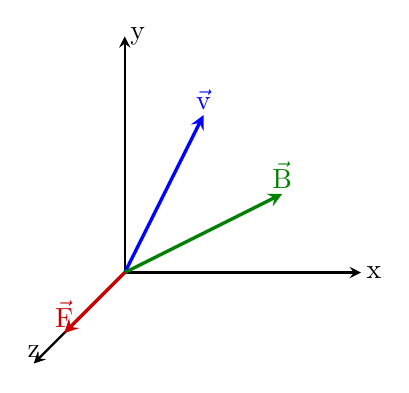
\begin{tikzpicture}[
		scale=1.0,
		%Option for nice arrows
		>=stealth, %
		inner sep=0pt, outer sep=2pt,%
		axis/.style={thick,->},
		wave/.style={very thick,color=#1,smooth, ->},
		polaroid/.style={fill=black!60!white, opacity=0.3},
	]
		% Colors
		\colorlet{darkgreen}{green!50!black}
		\colorlet{lightgreen}{green!80!black}
		\colorlet{darkred}{red!50!black}
		\colorlet{lightred}{red!80!black}

		% Frame
		\coordinate (O) at (0, 0, 0);
		\draw[axis] (O) -- +(3, 0,   0) node [right] {x};
		\draw[axis] (O) -- +(0,  3, 0) node [right] {y};
		\draw[axis] (O) -- +(0,  0,   3) node [above] {z};
		
		\draw[wave = blue] (O) -- +(1,  2,  0) 
			node [above] {$\vec{\uspeed}$};
		\draw[wave = darkgreen] (O) -- +(2,  1,  0) 
			node [above] {$\vec{\umfieldb}$};
		\draw[wave = lightred] (O) -- +(0,  0,  2) 
			node [above] {$\vec{\uforce}$};
	\end{tikzpicture}
\end{center}
þar sem krafturinn verkar einmitt hornrétt á tvo vigra. Þá leiðir til þess
að krafturinn er ekki samsíða hreyfi stefnunni. Dæmi um þetta væri segulsviðið
sem myndast umhverfis leiðara, það myndast hornrétt á hreyfistefnu rafeindanna
í leiðaranum. Stærð kraftins er hægt að finna með
\begin{align*}
	\left| 
	\vec{\uforce} \right|
		&= \left| \uchargeq \left( \vec{\uspeed} 
			\times \vec{\umfieldb}  \right) \right| 
			\\
		&= \uchargeq \left|  \vec{\uspeed}  \right| \left| \vec{\umfieldb} \right| 
			\sin(\theta)
\end{align*}
þar sem $ v = \left|  \vec{\uspeed}  \right| $ er lengd hraðavigursins og
$B = \left| \vec{\umfieldb} \right|$ er lengd segulsviðsvigurs. Þá er $\theta$
hornið á milli vigrana $\vec{\uspeed}$ og $\vec{\umfieldb}$, hægt er að finna
hornið á milli þeirra með að leysa út $\cos(\theta) | \vec{\umfieldb} |
| \vec{\uspeed} | = \vec{\umfieldb} \cdot \vec{\uspeed}$.
\begin{formalexample}
	Rafeind ferðast í lárréttu plani, hornrétt á rafeinda í planinu er segulsvið.
	Hraði rafeindarinnar er $\SI{15e3}{\m\per\s}$ og styrkur segulsviðsins er
	$\SI{0.5e-4}{\tesla}$. Í vigurformi er það
	\begin{align*}
	\vec{\uspeed} &= 
		\left( 
		\begin{array}{c} 
			$\SI{15e3}{\m\per\s}$ \\
			$0$ \\
			$0$ \\
		\end{array} 
		\right)
	&
	\vec{\umfieldb} &= 
		\left( 
		\begin{array}{c} 
			0 \\
			$\SI{0.5e-4}{\tesla}$ \\
			0 \\
		\end{array} 
		\right)		
	\end{align*}
	\vspace{4 ex}
	Fyrst þarf að setja upp hnitakerfi, þá er valið að láta x-ásin vera samsíða
	hreyfistefnu rafeindarinnar, þar sem hornið á milli vigrana er $\theta = 
	\ang{90}$ vegna þess að þeir eru hornréttir á hvorn annan þá er
	stærð kraftsins gefin við
	\begin{align*}
		F 	&= 
			\uchargeq
			\left|  \vec{\uspeed}  \right| \left| \vec{\umfieldb} \right| 
				\sin(\theta) \\
			&= \uunitcharge \times \SI{15e3}{\m\per\s} \times \SI{0.5e-4}{\tesla} 
				\times \sin(\ang{90}) \\
			&= \SI{12.45e-20}{\N}
	\end{align*}
	sem er afar lítill kraftur sem verkar á rafeinda.
\end{formalexample}

\section{Straumur og segulsvið}
Þegar rafeindir eru á hreyfingu er það kallaður rafstraumur eða straumur,
hægt er að lýsa straumi með hraða og magni. Þeas. flæðið af rafeindum, eða
hleðslu er stjórnað af fjölda þeirra og magnið fyrir einhvern bút af leiðara á
tímaeiningu segir til um hraða þeirra.



\subsection{Beinn leiðari}

\subsection{Spóla}

\section{Lögmál Biot-Savart}

\section{Hleðsla í segulsviði}

\section{Segulflæði}



%\chapter{Rafrásir}
% Intro to chapter 
%
%\setlength{\marginparwidth}{3cm}

\newpage

\section{Inngangur}

Við lifum í heimi sem er umlukinn ýmiskonar tækni. Við notum tækni í flestu sem við tökum okkur fyrir hendur á hverjum degi. Þegar við vöknum þá er það vekjaraklukka sem vekur okkur flest. Við notum ristavélar, notum ísskápa, notum farsima, keyrum bíla og jafnvel notum tækni til að bjarga lífi okkar í formi gangráða og svo framvegis. Mestöll þessi tækni hefur það sameiginlegt að það sem gefur tæknini hæfni til að virka sem skildi er rafmagn.
\\ \\
Fyrir hinn almenna notanda þá getur tæki sem keyrir á rafmagni verið dularfullt og flókið. Ef tekinn er farsimi eða fartölva inn í djúpustu frumskóga heims til frumstæðra þjóðflokka þá getur tæknin sem keyrir tækin virðst sem galdrar eða kraftaverk.
\\ \\
Bók þessari er ætluð þann tilgangur að gefa hinum almenna framhaldsskólanema innsýn inn í hvað rafmagn er, rafmagn virkar og hvernig rafmagn getur verið nýtt til að veita okkur hið tæknivædda umhverfi sem við lifum í.


\section{Hvað er rafmagn?}
Til að svara því hvað rafmagn er þá þurfum við að kíkja i heim atómana. Atom eru byggingarblokkir efnis, semsagt það eru atom í öllu efni hvort sem það er gull, sandur eða loftið sem við öndum að okkur. Þegar atom koma saman þá mynda þau efni og geta þá á einfaldann hátt talist byggingakubbar alls heimsins. Svipað og lego þegar það er samsett myndar kastala, bíla o.s.frv. þá mynda atóm þegar þau eru samsett allt það efni sem við vitum um. 
\\ \\ 
\marginpar{ \hspace{0pt} Rafeind geymir örlitla rafhleðslu.}
Kjarni atóma getur ýmist verið hlaðinn eða óhlaðinn rafeindum. Við réttar aðstæður þá er hægt að láta atom gefa frá sér, eða taka við rafeindum þegar óhlaðin atóm eru sett við hlið hlaðinna. Þegar þetta gerist þá kemst ákveðin hreyfing á rafeindirnar og það myndar, þegar milljónir rafeinda hreyfast í einu, það sem við köllum rafstraum í dag. Mynd 1 sýnir mynd af þessu ferli. Þetta er mjög einfölduð mynd en flestar efnafræði eða eðlisfræðibækur geta gefið betri innsýn inn í þetta ferli, þó er þessi útskýring nægjanleg fyrir það efni hér er fjallað um. 

\begin{figure}
\center
\includegraphics[bb=0 0 408 158]{fig_electrons.jpg}
\caption{Hreyfing rafeinda milli atóma.}
\end{figure}

\section{Grunn einingar rafmagns.}

Rafmagn er hugtak sem í raun er búið til úr þremur grunn einingum, viðámi, straum og spennu. Við getum ýmindað okkur þessi þrjú hugtök í sambandi við rör fyllt af vatni sem flæðir í gegn. Viðnámið taknar það þegar rörið þrengist og gerir vatninu erfiðara um vik að flæða. Straumurinn er magnið af vatni sem flæðir á hverjum stað í rörinu fyrir sig. Spennan er þá þrýstingurinn bakvið vatnið sem lætur það flæða. Nú getum við heimfært þessa líkingu yfir á rafrásir þar sem straumurinn af vatni er straumur af rafeindum, spennan er þrýstingurinn bakvið rafeindirnar myndaðar af rafeindaflæði inn á rasina og viðnám breytir flæði rafeinda, og þar með breytir straumflæði rásarinnar.

\begin{itemize}
\item Spenna er táknuð með stafnum V sem stendur fyrir "Volt". Við höfum öll séð merkingu á batteríum út í verslunum þar sem stendur 9V, 5V o.s.frv. Einnig eru merkingar með spennu gefnar á spennugjöfum við fartölvur, gsm síma og annarskonar tæki sem hlaða rafmagni inn á rafmagnstæki. Volt er skilgreint sem vinnan sem þarf að vera framkvæmd til að flytja rafhleðslu eitt coulomb á milli tveggja punkta. 1 coulomb er skilgreint sem 6.241*10\textsuperscript{18} rafeindir. Ef vinnan er jöfn einu joule þá er spennan á milli þeirra eitt volt. Þessi eining, volt, er einfaldlega hugsuð sem "þrýstingurinn" sem nauðsynlegur er til að færa nægann straum yfir á viðkomandi tæki. 

\item Straumur er táknaður með stafnum I, en er skrifað sem einingin "Ampere". Þetta gefur til kynna að ákveðið magn rafeinda hafi flætt framhjá tilteknum punkt á rafrás á ákveðnu timabili. Eitt Ampere er eitt coulomb á sekúndu. Raftæki geta dregið að sér straum, eða fengið straum þrýst inn á sig með spennu, en straumur getur ekki undir eðlilegum kringumstæðum flætt sjálfstætt.

\item Viðnám er táknað með stafnum R, en er skrifað með gríska stafnum $\Omega$ sem stendur fyrir "Ohm". Viðnám er oft sett inn á rafrásir til að breyta spennu og/eða straum.
\end{itemize}

\section{Ohm lögmálið.}
Eitt mikilvægasta lögmál rafmagnsfræðinnar er kalla "Ohm lögmálið". Þetta er sett upp sem stærðfræðiformúla:
\begin{equation}
V=IR
\end{equation} eða \\ 
\begin{center} Spenna = Straumur * Viðnám \end{center}
Þessi jafna lýsir samhengi milli þessara þriggja þátta sama hlutarins (Rafmagns). En þegar einni stærð er breytt þá breytast hinar stærðirnar um leið.
Með einfaldri algebru þá er hægt að sjá samhengi annara þátta jöfnunar. \\ \\
Fyrir straum:
\begin{equation}
I=\frac{V}{R}
\end{equation}
Fyrir viðnám:
\begin{equation}
R=\frac{V}{I}
\end{equation}
Með því að beita þessum formúlum þá er hægt að leysa stórann hluta allra vandamála sem einstaklingur er líklegur til að lenda á. \\ \\

\begin{enumerate}
\item Viðnáms dæmi.
	\begin{enumerate}
	\item Ef rás vinnur á 5V spennu og 3A straum. Hvað er viðnámið stórt? \\
		\begin{equation}
			\begin{split}
			V&=IR \\
			5V&=3A*R \\
			R&=\frac{5V}{3A}\\
			R&=1.66\Omega
			\end{split}
		\end{equation}
		Semsagt, samkvæmt lögmáli ohm, þá er stærð viðnámsins 1.6$\Omega$. Takið eftir að skref þrjú útreikningsins passar við
		eina útgáfu Ohm lögmálsins hér að ofan.
	\item Ef rás vinnur á 10V spennu og 5mA straum. Hvað er viðnámið stórt?
		\begin{equation}
			\begin{split}
				V&=IR \\
				10V&=0.01A*R \\
				R&=\frac{10V}{0.01A} \\
				R&=1000\Omega
			\end{split}
		\end{equation}
		Takið eftir að þúsund $\Omega$ er oft skrifað sem 1k$\Omega$. Þetta er venja innan rafmagnsfræðinnar, ásamt því að eitt mA er eitt milli ampere, eða 0.001 Ampere.
	\end{enumerate}
\item Straum dæmi.
	\begin{enumerate}
	\item Ef rás vinnur á 5V spennu, og hún fer gegnum 1k$\Omega$ viðnám. Hver er þá stærð straums rásarinnar?
		\begin{equation}
			\begin{split}
			V&=IR \\
			5V&=I*1k\Omega \\
			I&=\frac{5V}{1k\Omega} \\
			I&=0.005A \\
			&=5mA
			\end{split}
		\end{equation}
		Takið eftir hvernig breytt er milli k og þúsund, einnig þá hvernig farið er milli A og mA.
	\end{enumerate}
\item Spennu dæmi.
	\begin{enumerate}
		\item Ef rás hef 2.4k$\Omega$ viðnám, og straum sem fer gegnum það sem er 3mA. Hver er þá stærð spennunnar?
		\begin{equation}
			\begin{split}
			V&=IR \\
			V&=2.4k\Omega*3mA \\
			&=2400\Omega*0.003A \\
			V&=72V
			\end{split}
		\end{equation}
	\end{enumerate}
\end{enumerate}

\section{Aðrar rafeiningar.}
\subsection{Þéttar}
þéttar eru ein grunneininga rafmagnsfræðinnar í íhlutum talið. Viðnám og þéttar eru nægir íhlutir til að framkvæma ýmsar
aðgerðir með rafrásum. Hægt er að horfa á þétti sem hálfgert forðabúr. Þegar auka rafmagn er til staðar þá dregur þéttirinn
það í sig, auk þess sem það jafnar út ýmsar ójöfnur eins og þegar það kemur stutt tímabil þar sem rafmagn vantar, þá getur þéttir
veitt rafmagni úr forðabúrinu til að jafna út þessa ójöfnu svo tækið virki sem skildi. Einingin sem notuð er til að gefa til kynna
hleðslu þétta heitir ''Farad'' eftir englendingnum Michael Faraday. Eins farad þéttir getur hlaðið inn á sig ramagni sem nemur einu coloumb á hvert volt (1C/V) 
eða eina amper sekúndu á volt (1As/V).
\begin{figure}[htb]
	\center
		\includegraphics[bb=0 0 252 262,scale=0.3]{capnres.png}
		\caption{Tákn fyrir þétta (vinstri) og viðnám (hægri).}
\end{figure}

\subsection{Spólur.}
Spólur eru íhlutir í rafrásum sem hafa tvo eiginleika. Þær búa til segulsvið ásamt því að ''hægja'' á straum. Fyrri eiginleikinn nýtist við það að útbúa 
segulmagn og loftnet. Seinni eiginleikinn hefur aðal tilgang í riðstraumsrásum (AC) þar sem spólur nýtast til að breyta lögun rafmerkja. Eining fyrir styrk
spóla er ''Henry''.
\begin{figure}[htb]
	\center
		\includegraphics[bb=0 0 269 130,scale=0.3]{./pictures/inductor.png}
		\caption{Tákn fyrir spólu.}
\end{figure}

\section{Rað og hliðtengingar.}
Við höfum þegar séð hvernig reikna á straum, spennu og viðnám við einföldustu aðstæður. En nú ætlum við að skoða hvernig við reiknum þessa hluti í flóknari
rafrásum.
\begin{figure}[htb]
	\center
		\includegraphics[bb=0 0 873 552,scale=0.3]{./pictures/demo_circ_serpar.png}
		\caption{Einföld rafrás með hlið og raðtengdum íhlutum.}
\end{figure}
Þegar íhlutir eins og viðnám og þéttar eru settir í rásir í rað, eða hliðtengingum þá breytast eiginleikar rásarinnar samkvæmt því. 

\subsection{Viðnám.}
\begin{figure}[htb]
	\center
		\includegraphics[bb=0 0 761 309,scale=0.3]{./pictures/res_parser.png}
		\caption{(a)Hliðtend viðnám. (b)Raðtengd viðnám.}
		\label{fig:res_parser}
\end{figure}
Þegar hlutir gerast! Sjá mynd ~\ref{fig:res_parser}.

\subsection{Þéttar.}
\begin{figure}[htb]
	\center
		\includegraphics[bb=0 0 1056 370,scale=0.3]{./pictures/cap_parser.png}
		\caption{(a)Hliðtendir þéttar. (b)Raðtengdir þéttar.}
		\label{fig:cap_parser}
\end{figure}
Þá gerast hlutir! Sjá mynd ~\ref{fig:cap_parser}.


%\input{sections/electric_forces}
%\input{sections/electric_fields}
%\input{sections/electric_potentials}
%\input{sections/electric_condensors}
%\input{sections/electric_magnetic_force}
%\input{sections/electric_magnetic_inductance}
%\input{sections/electric_electromagnetic_force}

% 
% Modern physics
% 

\part{Nútíma eðlisfræði}
%
% A container for modern physics
%

%\input{sections/reference_frames}
%\input{sections/special_relativity}
%\input{sections/star_formation}
%\input{sections/quantum_physics}
%\input{sections/radioactivity}
%\input{sections/kinetic_entropy}


\bibliographystyle{plain}	
\bibliography{bib/pictures}

\end{document} 
